\documentclass[12pt,a4paper,twoside,openright]{report}

\usepackage{graphicx}
\usepackage{tabularx}
\usepackage{subfigure}
\usepackage{afterpage}
\usepackage{amsmath,amssymb}
\DeclareMathOperator*{\argmax}{argmax} % thin space, limits underneath in displays
\usepackage{rotating}  
\usepackage{fancyhdr}  
\usepackage[numbers]{natbib}
\usepackage{algorithm}
\usepackage[noend]{algpseudocode}
\usepackage[scriptsize]{caption}
\usepackage{url}
\hyphenation{a-gen-tiz-za-zio-ne}

\usepackage[right=4.5cm,left=4.5cm,top=4.5cm,bottom=4.5cm]{geometry}
\linespread{1.1}

\usepackage[english]{babel}
%\usepackage[latin1]{inputenc}
\usepackage[utf8]{inputenc}
\renewcommand{\captionfont}{\normalfont \sffamily \itshape \small}

\pagestyle{plain}
\AtEndDocument{\thispagestyle{plain}}

\begin{document}
\pagenumbering{gobble}
\thispagestyle{empty}
%\begin{titlepage}
\vspace*{-1.5cm} \bfseries{
\begin{center}
\large
POLITECNICO DI MILANO\\
\normalsize
Corso di Laurea Magistrale in Ingegneria Informatica\\
Dipartimento di Elettronica, Informazione e Bioingegneria\\
\begin{figure}[htbp]
\begin{center}

\includegraphics[width=5cm]{pictures/logopm.png}
\end{center}
\end{figure}
\vspace*{0.3cm} \LARGE


\textbf{Monte Carlo Tree Seach for Sokoban}\\

  
\end{center}
\vspace*{3.0cm} \large
\begin{flushleft}

Relatore:\\
Prof. Pier Luca LANZI \\

\end{flushleft}
\vspace*{1.0cm}
\begin{flushright}

Tesi di Laurea di:\\
Fabio MAROCCHI, Matr. 858408\\
Mattia CRIPPA, Matr. 854126

\end{flushright}
\vspace*{1cm}
\begin{center}

Anno Accademico 2016-2017
\end{center}
\clearpage
}

\thispagestyle{empty} \normalfont \cleardoublepage
%\vspace{17cm}

%\large
\begin{flushright}
\itshape{A tutti i nostri cari}
\end{flushright}

\thispagestyle{empty}\cleardoublepage
\newpage
\chapter*{Sommario}
\textit{Monte Carlo Tree Search} (MCTS) è uno degli algoritmi più utilizzati nel campo dell'intelligenza artificiale applicata ai giochi da tavolo e ai giochi di carte.
Lo scopo di questa tesi è di valutare le prestazioni dell'algoritmo MCTS applicato al puzzle game Sokoban, confrontandolo con un altro algoritmo ben noto, \textit{Iterative Deepening A*}, che ha dimostrato di avere un discreto successo in questo puzzle game.
In questa tesi applichiamo MCTS e IDA* a Sokoban e Samegame, un altro puzzle game. Sviluppiamo anche una serie di ottimizzazioni conosciute per MCTS e IDA* e ne presentiamo alcune nuove. Infine, valutiamo gli effetti delle ottimizzazioni su entrambi i domini. I nostri risultati mostrano che in Samegame la formula UCB1-Tuned ottiene prestazioni migliori rispetto a SP-MCTS, una versione single player di MCTS che ha ottenuto buoni risultati in quel dominio in passato. In Sokoban, la migliore configurazione del MCTS usa l'UCT standard con l'aggiunta delle ottimizzazioni proposte denominate Node Elimination e Cycles Avoidance, che portano ad un drastico aumento del numero di livelli risolti dall'algoritmo MCTS in Sokoban. Nonostante ciò, anche con una serie di miglioramenti che possono essere trovati in letteratura, che sono stati ampiamente utilizzati e hanno raggiunto risultati di successo, l'algoritmo MCTS non ha potuto eguagliare le prestazioni di IDA* in termini di numero di livelli risolti. Per questo motivo IDA* rimane ancora il miglior algoritmo per Sokoban.\cleardoublepage
\newpage
\chapter*{Abstract}
\textit{Monte Carlo Tree Search} (MCTS) is one of the most used algorithm in the field of Artificial Intelligence applied to board and card games.
The aim of this thesis is to evaluate the performance of MCTS algorithm applied to the puzzle game Sokoban, comparing it to another well known algorithm, \textit{Iterative Deepening A*}, which has been proven to be quite successful in this puzzle game.
In this thesis we apply MCTS and IDA* to Sokoban and Samegame, another puzzle game. We also develop a series of known optimizations to MCTS and IDA* and present some new ones. Finally, we evaluate the effects of the optimizations on both domains. Our results show that in Samegame the UCB1-Tuned formula performs better than SP-MCTS, a single player version of MCTS that obtained good results in that domain in the past. In Sokoban, the best MCTS configuration uses the standard UCT with the addition of the proposed optimizations called Node Elimination and Cycles Avoidance, which lead to a drastic increase in the number of levels solved. Despite this, even with a set of enhancements that can be found in the literature, which have been widely used and have achieved successful results, the MCTS algorithm could not match IDA* performance in terms of number of solved levels. For this reason IDA* still remains the best algorithm for Sokoban.\cleardoublepage
\chapter*{Acknowledgments}

We would like to thank our supervisor Prof. Pier Luca Lanzi for the guidance provided during our research and for helping us with feedbacks and suggestions.

\medskip\noindent
We also thank our families and friends for their support. We wouldn't have been able to reach this goal without them.

\begin{flushright}
\textit{Fabio and Mattia, 06/04/2018}
\end{flushright}
\thispagestyle{empty} \vspace*{.75truecm} \normalfont \cleardoublepage
\tableofcontents
\cleardoublepage
\listoffigures
\cleardoublepage
\listoftables
\cleardoublepage
\listofalgorithms
\pagenumbering{gobble}
\thispagestyle{empty} \vspace*{.75truecm} \cleardoublepage
\pagestyle{plain}
%\pagestyle{plain}\renewcommand{\chaptermark}[1]{\markboth{\chaptername\ \thechapter.\ #1}{}} 
%\renewcommand{\sectionmark}[1]{\markright{\thesection.\ #1}}         
%\fancyhead[LE,RO]{\bfseries\thepage}    
                                        
%\fancyhead[RE]{\bfseries\leftmark}    
%\fancyhead[LO]{\bfseries\rightmark}     
%\renewcommand{\headrulewidth}{0.3pt} 
%\raggedbottom

\pagenumbering{arabic}
\chapter{Introduction}
\label{Introduzione}
This thesis focuses on the application of Artificial Intelligence (AI) to puzzle games. This field was born in the ’50s and the first AI algorithms, developed for two-players-board games (like Checkers and Chess), were able to play only final moves of the game or they could only play at beginners level. In the following years, these programs could compete against human-expert players due to more advanced techniques that have been developed. In some cases, it has been possible to solve a game, i.e. predict the result of a game played from a certain state in which all the players did the optimal moves.

\medskip\noindent
The aim of this thesis is to evaluate the performance of \textit{Monte Carlo Tree Search} (MCTS) applied to the puzzle game Sokoban, a single-player computer game in which the player inside a maze has to push boxes to assigned positions. Only one box at a time can be pushed and the boxes can not be pulled.

\medskip\noindent
MCTS has been introduced in 2006 by Rèmi Coulom \cite{coulom:inria-00116992}, combining tree search with Monte-Carlo evaluations which introduced independence from domain knowledge and a fine-grained control of the growth of the tree. Shortly after, Kocsis and Szepesvàri \cite{Kocsis:2006:BBM:2091602.2091633} formalized this approach into the \textit{Upper Confidence Bounds for Trees} (UCT) algorithm, which nowadays is the most used algorithm of the MCTS family. In contrast with the classical AI algorithms (like Minimax), that completely explore the search tree, MCTS builds up a tree in an incremental and asymmetric manner guided by many random simulated games. In this way it can explore only the most promising areas of the tree. Moreover, the exploration can be stopped at any time returning the current best result, this make MCTS very efficient in terms of time and memory. Kocsis and Szepesvàri were also able to prove that, with enough iterations of the algorithm, MCTS converges to the same result of Minimax.

\medskip\noindent
Due to the successful application of MCTS algorithm to many board games, in this thesis we evaluate its efficiency in Sokoban comparing it to another well known algorithm, \textit{Iterative Deepening A*}, which has been proven to have a huge success in this puzzle game \cite{Junghanns99pushingthe}.

\section{Thesis outline}
The structure of the thesis is describe in the following:
\begin{itemize}
    \item Chapter 2 provides a background of Sokoban, outlining its rules and complexity. It also provides a description of the used algorithm \textit{Iterative Deepening A*} and its enhancements for the chosen puzzle.
    \item Chapter 3 reports the state of art of the \textit{Monte Carlo Tree Search} (MCTS) algorithm, a description of it and enhancements that have been developed. It also describes a case study, represented by Samegame, in with MCTS has been successfully used.
    \item Chapter 4 presents our solution to the puzzle solving problem, describing the domain dependent/independent enhancements used to improve performance.
    \item Chapter 5 outlines all the experiments used in this thesis in order to compare the efficiency of the different algorithms in the different domains. Then compares the results obtained by the algorithms in the proposed experiments in order to determine which algorithm has better performance in each domain.
    \item Chapter 6 presents an analysis of the results with respect to the aim of the thesis and also set out possible further improvements that can be integrated in this work. 
\end{itemize}
\chapter{Puzzles and AI}
\label{puzzles}
In this chapter we provide a background of Sokoban, describing the game rules and its complexity. We then give a short introduction of the classic algorithm \textit{Iterative Deepening A*} and some of its enhancement which have been used in the selected game and that can be found in literature.

\medskip\noindent
Puzzles have been popular since the dawn of mankind, and are known for stimulating brain activity and mental welfare as well as simply being fun. A puzzle is a pastime that consists of a problem or a riddle that tests the ingenuity of those who are called to solve it. There are many types of puzzles that can test different problem-solving skills including logic, pattern recognition, sequence solving, and word completion. The various types of solutions may require structuring a form or creating a certain order. The term puzzle usually refers to single-player games which are enjoyable to play. By definition a puzzle should have a solution which is aesthetically pleasing and gives the user satisfaction in reaching it \cite{journals/icga/KendallPS08}.

\medskip\noindent
In the last decades puzzles have become a more interesting field in computer science due to the fact that finding solutions for them, often requires the recognition of patterns. This makes puzzles suitable to be solved using artificial intelligence agents. A lot of different approaches have been used trying to find a solution to the puzzle solving problem and it has been discovered that specific artificial intelligence methods can work better in some domains rather than in others.

\medskip\noindent
A large amount of different puzzles and artificial intelligence applied to them can be found in literature, and one of the most used algorithm is \textit{Iterative Deepening A*}. This algorithm has been employed to solve different puzzle games such as \textit{n}-Puzzle and Sokoban obtaining good results \cite{journals/icga/KendallPS08}.

\section{Sokoban}\label{sec:sokoban}
Sokoban is a single-player computer game created by Hiroyuki Imabayashi in 1981 and published in December 1982 by Thinking Rabbit, a software house based in Takarazuka, Japan (the japanese name "Sokoban" can be translated as "warehouse keeper"). A level in Sokoban, as shown in Figure \ref{fig:sokobanlevel}, consists of a series of rooms and passageways on a grid, in which are scattered a series of boxes (also called stones) and goals (the dashed area). The number of boxes must match the number of goals.

\begin{figure}[!h]
\centering
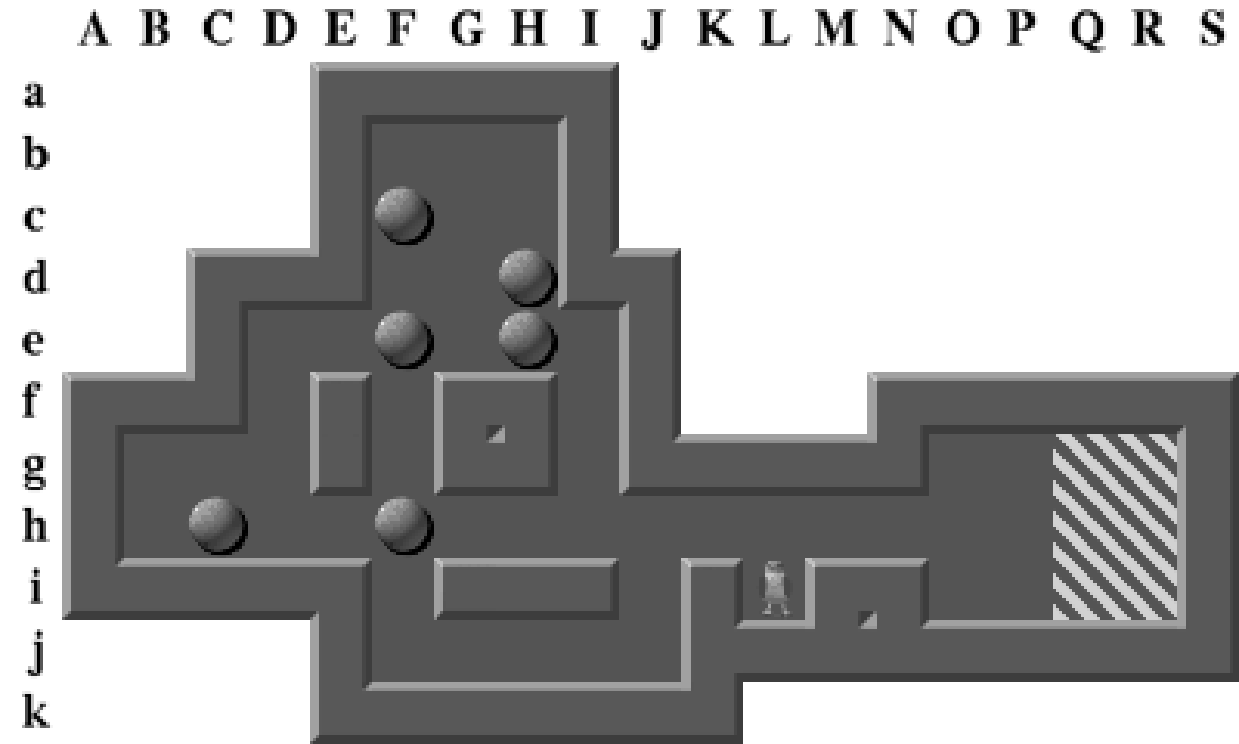
\includegraphics[width=0.7\linewidth]{pictures/sokoban_1.png}
\caption[Example of a Sokoban level]{Example of a Sokoban level \cite{Junghanns99pushingthe}}
\label{fig:sokobanlevel}
\end{figure}

\subsection{Rules}
The goal of the game is to move every box on a goal square. The player controls a character (which we will refer to as the \textit{pusher}) that can move around the level orthogonally on empty squares and goal squares. It cannot cross boxes or walls. If the player tries to move on a square occupied by a box, the box is pushed by one square in the direction of the movement, provided that the target square is either empty or an unoccupied goal. The boxes cannot be pulled, so some moves can be irreversible.

\medskip\noindent
Once every box is on a goal square, the level is solved. In addition to solving the level, the player can also try to find an optimal solution. In Sokoban, the optimality of the solution is usually measured by minimizing one of two metrics:
\begin{itemize}
    \item The total number of pushes, i.e. moves which cause the box to change its position;
    \item The total number of moves, whether they are simple pusher movements or actual box pushes.
\end{itemize}
The canonical metric used is the number of pushes. An optimal solution for a sokoban level can range from a minimum of one push and one move (see level 44 of the Microban set \cite{microban}) to hundreds of pushes and thousands of moves. Sokoban uses a standard format for level files and many level sets have been created by users and enthusiasts\footnote{Most level sets can be found at http://www.sourcecode.se/sokoban/levels}.

\medskip\noindent
One aspect that differentiates it from most puzzles studied in the literature is that an irreversible move can lead to a state that we call \textit{deadlock}, from which no solution can be found. There are two main types of deadlock:
\begin{itemize}
    \item A \textit{simple deadlock} happens when a box is moved on a square from which it cannot reach any goal, regardless of the position of other boxes.
    \item A \textit{freeze deadlock} happens when a box is moved on a non goal square and becomes immovable. That is, when it can't be pushed again. This often includes other boxes that become immovable in turn.
\end{itemize}
Simple deadlocks only depend on the position of a single box, so they can be computed once per level and are fairly easy to identify. Freeze deadlocks instead require interaction between multiple boxes so they must be dealt with at run time. Anyhow, the game is not equipped with deadlock detection mechanisms, so the player can actually continue to play and interact with other boxes despite the deadlock situation. 

\medskip\noindent
In addition to the two main deadlock types, there are other situations that will eventually lead to one of the mentioned deadlocks, but might be recognized earlier. \textit{Corral deadlocks} are defined as a situation in which a portion of the board can't be reached by the player because its access is blocked by boxes and there's no way to get all of those boxes to a goal square. \textit{Bipartite deadlocks} happen when all boxes could still reach a goal, but there's an overlap on the goals they can reach, meaning that not all goals can be occupied at the same time. In order to solve a Sokoban problem, an algorithm (as well as a human player) must be able to recognize these situations early to prune them and reduce the search space. A few examples of deadlocks are represented in Figure \ref{fig:deadlock}.
\begin{figure}[!h]
\centering
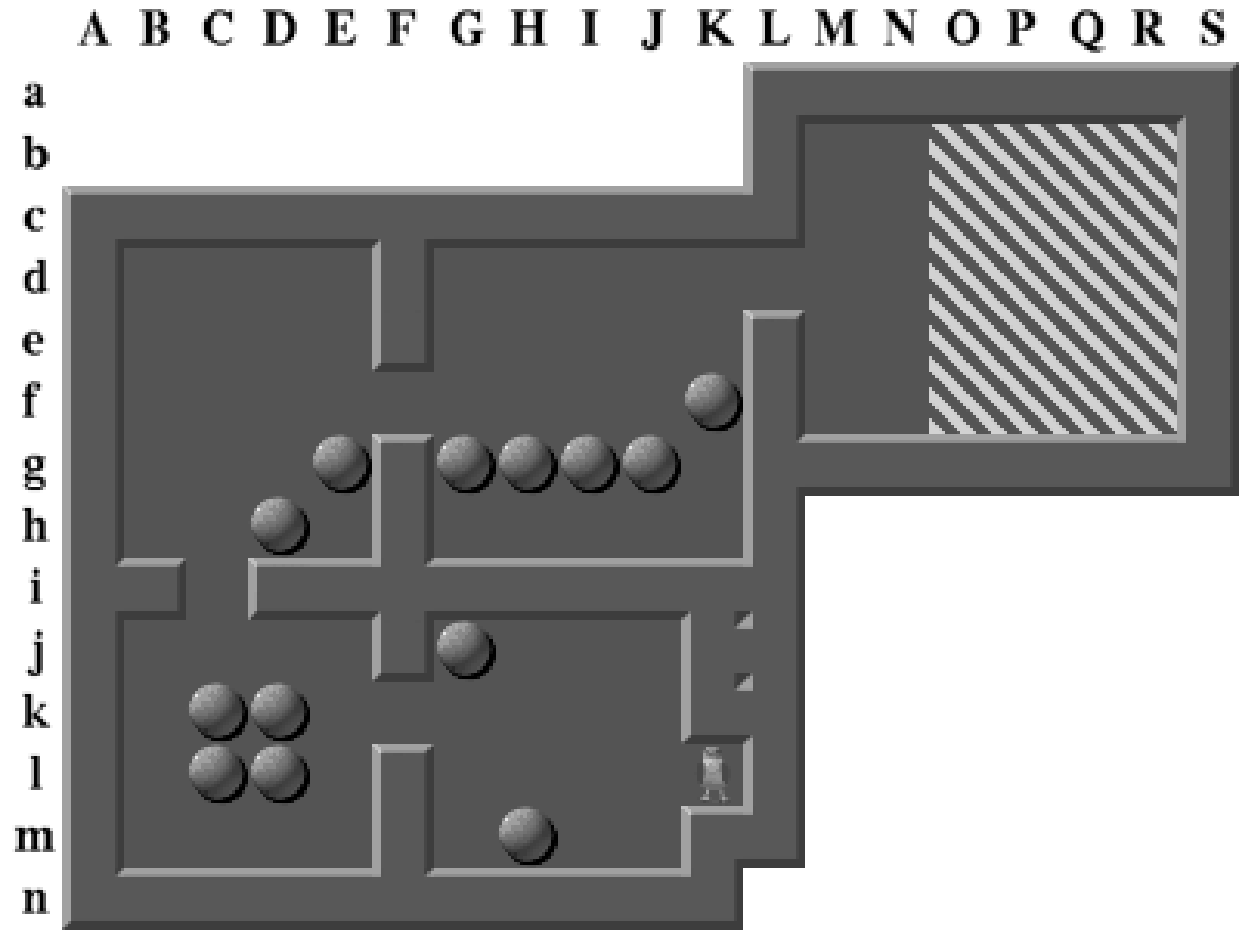
\includegraphics[width=0.7\linewidth]{pictures/sokoban_deadlock.png}
\caption[Deadlock example]{Deadlock examples: upper-left: Corral deadlock; upper-right: Corral deadlock; lower-left: Freeze deadlock; lower-right: Simple deadlock \cite{Junghanns99pushingthe}}
\label{fig:deadlock}
\end{figure}

\subsection{Complexity}
Assuming that our goal is to minimize the number of pushes, we can analyze the game by considering only push moves on boxes that are reachable from the player current position. Considering that in the standard set the number of boxes ranges from 6 to 34 and that we can have up to 4 moves per box, the branching factor can potentially reach a maximum of 136. Of course part of the complexity of Sokoban relies on the constraints that come from the risk of creating deadlocks, so in most of the levels the boxes are densely packed, meaning that the number of available moves is considerably lower. Level 1 (Figure \ref{fig:sokobanlevel}), with only 6 boxes is one of the easiest levels. We can compute an average branching factor $b$ of 3.07, and with a solution length $d$ of 97, the game-tree complexity becomes approximately $10^{47}$. Suppose that we have a similar boxes-to-moves ratio for all levels, with an average number of boxes of 16 and an average solution length of 284.8, we can roughly estimate the average game-tree complexity as $10^{260}$. Since the game rules don't contemplate a limit in the number of moves, and the pusher can retrace its steps, the game length can be considered potentially unlimited. Therefore, to solve a Sokoban puzzle, one should avoid cycles during the search. Junghanns et al. \cite{Junghanns99pushingthe} computed the upper bound for the state-space complexity of Sokoban on a $20\times 20$ board with walls on the perimeter, as $\binom{s}{b}m$ where $s$ is the total number of squares, $b$ is the maximum number of boxes and $m$ is the number of possible pusher positions. This yields a result of $10^{98}$. With an average number of squares of 77 (excluding squares that would cause simple deadlocks) and an average number of boxes of 16, the average state-space complexity of the standard levels suite is approximately $10^{18}$. Sokoban has also been shown to be NP-hard and P-space complete \cite{Pspace-complete97sokobanis} and is considered challenging for both humans and programs.

\section{Iterative Deepening A*}
\textit{Iterative Deepening A*} is one of the most successful methods for puzzle solving that can be found in the literature and it is based on a classical planning approach.

\subsection{Overview}
%\begin{algorithm}
%  \caption{\textbf{A*}}\label{alg:astar}
%  \begin{algorithmic}
%  \Function{Astar}{$\textit{s\textsubscript{0}}$}
%    \State create root node \textit{n\textsubscript{0}} with state \textit{s\textsubscript{0}}
%    \State create queue \textit{frontier} with node $s_0$
%    \While{ \textbf{not} \Call{IsEmpty}{frontier}}
%        \State $n \gets \Call{First}{frontier}$
%        \If{$\Call{IsGoal}{n}$}
%        \State \Return $\Call{BuildSolution}{n}$
%        \EndIf
%        \State $successors \gets \Call{GenerateSuccessors}{n}$
%        \State $\Call{AddToQueue}{frontier, successors}$
%        \State $\Call{Sort}{frontier}$
%    \EndWhile
%    \State \Return $failure$
%    \EndFunction
%  \end{algorithmic}
%\end{algorithm}

\textit{Iterative Deepening A*} (IDA*) is a variant of \textit{Iterative Deepening Depth-First Search} (IDDFS) that relies on heuristic evaluation to determine the threshold for the cut point of the current iteration. It was described by Richard Korf in 1985 \cite{Korf:1985:DIO:4433.4436}. 
IDDFS is an uninformed search method in which a depth limited depth-first search is repeatedly executed with increasing depth limit until a solution is found. At each iteration a full depth-first search is performed until either a solution is found or the entire search tree has been explored up to the depth limit $d$. If no solution has been found, $d$ is increased and the search is repeated. 

\medskip\noindent
The method inherits the low memory complexity of depth first search, while retaining completeness even in presence of unlimited trees. Optimality is preserved if all actions have constant cost.Similarly to IDDFS, IDA* proceeds in a depth-first manner with a depth bound, and once the whole tree for that bound has been explored, the search restarts with an increased bound. Unlike IDDFS, the threshold is not defined in terms of tree depth, but of heuristic evaluation. The method used to determine if the search can continue is based on A* evaluation. A* is an informed search algorithm first proposed in 1968 by Hart et al. \cite{Hart1968} as an improvement over Dijkstra's algorithm for finding the minimum cost path in a weighted graph. At each iteration it explores the node that minimizes
\begin{equation}
    f(n) = g(n)+h(n)
\end{equation}
where $g(n)$ is the cost of reaching node $n$ from the initial node and $h(n)$ is a heuristic estimate of the cost from node $n$ to the goal.

\medskip\noindent
In IDA* as in A*, in order to guarantee the optimality of the solution, the evaluation function $h$ must satisfy the following conditions:
\begin{itemize}
    \item Admissibility: $h(n)<h^*(n)$  with $h^*(n)$ being the perfect heuristic (the actual cost from $n$ to the goal in the optimal solution.
    \item Consistency: $h(n)\leq g(n') + h(n') -g(n)$ where $n'$ is a successor of $n$. 
\end{itemize}
If these condition are satisfied, and a solution is found, that solution is guaranteed to be optimal \cite{Hart1968}.

\subsection{The Algorithm}
IDA* initializes the search threshold as the heuristic value of the initial state $h(n_0)$. It then proceeds in a depth-first exploration until either the value $f(n) = g(n) + h(n)$ exceeds the threshold or there are no more successors. When one of these condition is satisfied, the search returns to the parent node and expands the siblings of the last explored node, exactly like in IDDFS. This produces an asymmetric search tree that grows guided by the heuristic function. The main advantage of this approach with respect to classic A* algorithm is that it runs in space that is linear in the maximum search depth, rather than exponential. Pseudocode for IDA* is showed in Algorithm \ref{alg:idastar}.

\begin{algorithm}
  \caption[IDA*]{\textbf{IDA*}}\label{alg:idastar}
  \begin{algorithmic}
      \Function{IDA*}{$s_0$}
        \State create root node $n_0$ with state $s_0$
        \State create solution $path$ with $n_0$
        \State $threshold \gets \Call{h}{n_0}$
        \While{result not found}
                \State $value \gets \Call{Search}{path,0,threshold}$
            \If{$value = RESULT$}
            \Return $path$
            \EndIf
            \If{$value = \infty$}
            \Return $failure$
            \EndIf
            \State $threshold\gets value$
        \EndWhile
    \EndFunction
    
    \Function{Search}{$path, g, threshold$}
        \State $n\gets \Call{Last}{path}$
        \State $f \gets g+\Call{h}{n}$
        \If{$f>threshold$}
            \Return $f$
        \EndIf
        \If{$\Call{IsGoal}{n}$}
            \Return $RESULT$
        \EndIf
        \State $min\gets\infty$
        \State $successors \gets \Call{GenerateSuccessors}{n}$
        \ForAll{$child$ \textbf{in} $successors$ }
            \State $\Call{Push}{path, child}$
            \State $cost \gets \Call{ActionCost}{child,n}$
            \State $t \gets \Call{Search}{path, g + cost , threshold}$
            \If{$t=RESULT$}
                \Return $RESULT$
            \EndIf
            \State $min\gets \Call{MIN}{min,t}$
            \State $\Call{Pop}{path}$
        \EndFor
        \Return $min$
    \EndFunction
  \end{algorithmic}
\end{algorithm}

\subsection{State of the art}\label{sokobanoptimizations}
IDA* has reached good results in Sokoban \cite{Junghanns99pushingthe} and in the 15-Puzzle (and derivatives) \cite{DBLP:conf/aaai/KorfT96}. 
In the context of Sokoban, the only documented method that can be considered state of the art is the program \textit{Rolling Stone} \cite{Junghanns99pushingthe}. It implements domain independent enhancements \cite{DBLP:journals/pami/ReinefeldM94} to prune the search tree and domain specific enhancements that make use of lower level searches to avoid deadlocks, obtain a tighter lower bound and reduce the search space.

\subsubsection*{Transposition Tables}
Transposition tables consists of data structures used to store information about visited states and are used to avoid cycles during the search and to reduce the branching factor. In Rolling Stone the heuristic evaluation of nodes is stored in the transposition table and updated according to the result of previous iterations. This allows the algorithm to improve the heuristic values and prune sub-trees more efficiently.

\subsubsection*{Move Ordering}
Children of a node are ordered based on the likelihood of leading to a solution. The move ordering scheme proposed was the following:
\begin{enumerate}
    \item \textit{Inertia} moves are considered first. Inertia moves are those moves that preserve inertia, meaning that they act on the same stone as the previous move.
    \item Then all moves that decrease the lower bound are tried (optimal moves), sorted by distance from the stone to its target goal.
    \item Finally, all non-optimal moves are tried, also sorted by distance to target goals.
\end{enumerate}

\subsubsection*{Deadlock Tables}
Deadlock tables make use of pattern database \cite{10.1007/3-540-61291-2_68} to match the current situation to precomputed tables of possible deadlock configurations. The tables are computed offline with all possible combinations of walls, stones and empty squares for a fixed-size region. The deadlock tables are implemented as decision trees, with internal nodes representing subpatterns and leaves representing whether the pattern is a deadlock or not. Junghanns et al. \cite{Junghanns99pushingthe} built two tables for regions of roughly 5x4 squares, that differed in the order the squares in the maze are queried.

\subsubsection*{Tunnel Macros}
A \textit{tunnel} is defined as a part of the maze where the maneuverability of the pusher is restricted to a width of one. These regions cannot have more than one box inside, otherwise they would cause a deadlock. In order to reduce the branching factor, we can collapse all pushes of a box inside a tunnel in a single move that makes the box exit that tunnel.

\subsubsection*{Goal Macros}
When the levels have all goal squares concentrated in a small area, if there are few entrances to this area, the problem can be decomposed in two sub-problems:
\begin{itemize}
    \item moving boxes to the entrances 
    \item placing boxes on goals
\end{itemize}
In some cases these two parts can be solved separately. With Goal Macros, the order in which goal squares must be filled to avoid deadlocks is precomputed, and when a box reaches an entrance the only move it can perform is the Goal Macro, that pushes it directly into its assigned goal.

\subsubsection*{Goal Cuts}
The move pruning of Goal Macros is backpropagated to previous states when a stone is pushed to a square with a Goal Macro at the end without interleaving other stone pushes.

\subsubsection*{Pattern Search}
Pattern search uses sub-problem searches to improve the lower bound and to identify deadlock patterns. It consists of repeated IDA* searches with patterns of more and more boxes. When a deadlock pattern is found, it's saved and used throughout the search in addition to those in the deadlock tables.
The basic algorithm performs the following steps:
\begin{enumerate}
    \item Create a test maze with the same walls and goals configuration but containing only the last moved box.
    \item Try to find a solution to the test maze.
    \item If no solution is found, the pattern is a deadlock. Return pattern.
    \item If a solution is found, add a box that is on a square that is needed for the solution. A square is needed for the solution if either the box or the man had to go through it in the solution found.
    \item If search effort is not exhausted, repeat from 2.
\end{enumerate}
Therefore the pattern search can terminate if the effort is reached, a deadlock was detected or no more stones can be added.
In particular, three types of specialized search has been implemented: 
\begin{itemize}
    \item Deadlock Search: specialized in finding deadlocks, it ignores states that are less likely to contain a deadlock to reduce the cost and be able to include more boxes in the search.
    \item Penalty Search: specialized in finding conflicts between boxes, is not allowed to take shortcuts, hence it might discover patterns ignored by the deadlock search. It's therefore more expensive and it evaluates less boxes with the same search effort.
    \item Area Search: specialized on finding deadlocks, it focuses on areas that are not accessible to the man. It incrementally includes all boxes that surround those areas, trying to find a deadlock. This is similar in concept to the PI-Corral pruning of the YASS solver \cite{yassscribbles}.
\end{itemize}

\subsubsection*{Relevance Cuts}
Relevance cuts is a forward pruning methods that removes moves that are considered not relevant. A move is relevant only if the previous $m$ moves influence it. The influence metric is defined based on the position of the boxes as follows:
\begin{itemize}
    \item Alternatives: The more alternatives exist on a path between two squares, the less the squares influence each other.
    \item Goal-Skew: for a given square $sq$, squares on the optimal path from $sq$ to its goal have a stronger influence than those off the optimal path.
    \item Connection: Two adjacent squares between which a stone can be moved freely influence each other more than two squares between which only the man can move freely.
    \item Tunnel: Influence remains constant inside a tunnel.
\end{itemize}

\subsubsection*{Overestimation}
Overestimation is based on the idea that a good non admissible heuristic might be closer to the optimal value than a poor admissible heuristic. Given the complexity of the problem, non optimal solution are acceptable. Overestimation allows every pattern found during pattern search to increment the lower bound. This will postpone "difficult" situations, giving up optimality but preserving completeness.
\chapter{Monte Carlo Tree Search}
\label{MCTS}
In this chapter we present the second chosen algorithm \textit{Monte Carlo Tree Search}, giving a description of this algorithm and of its improvements which can be found in literature. We also present and briefly describe rules and complexity of Samegame, a puzzle domain where \textit{Monte Carlo Tree Search} achieve good results.

\medskip\noindent
Traditional artificial intelligence methods require a good heuristic function to evaluate moves and could be unsuitable for those domains in which defining an heuristic using expert knowledge is particularly difficult. In these situations, Monte Carlo methods can make up for the lack of a solid heuristic by obtaining an approximate evaluation of the game-theoretic value of a move, by relying on the use of simulated playouts. The value of action $a$ in state $s$ can be expressed as
\[Q(s,a) = \frac{1}{N(s,a)}\sum^{N(s)}_{i=1}I_i(s,a)z_i\]
Where $Q(s,a)$ is the action-value function, $N(s,a)$ is the number of times action $a$ has been selected from state $s$, $N(s)$ is the number of visits through state $s$, $I_i(s,a)$ has value 1 if action $a$ was selected from $s$ in the $i-th$ playout and $z_i$ is the final reward of simulation $i$. Essentially, the value of an action is computed as the average reward obtained in the playouts in which that action was taken.

\medskip\noindent
Monte Carlo evaluation was initially applied to tree search as an alternative to ad-hoc evaluation functions to prune the search tree \cite{10.1007/11674399_5} \cite{Juille99methodsfor}. These methods had the drawback of having no game-theoretic guarantees on the optimality of the solution.
Monte Carlo evaluation was also applied to Markov Decision Processes with better asymptotic properties \cite{doi:10.1287/opre.1040.0145} \cite{Bai:2015:OPL:2801030.2717316}. First visit Monte Carlo evaluation for example, is an unbiased estimator for the action-value function, meaning that given enough samples, it will converge to the actual function.

\medskip\noindent
The algorithm known as Monte Carlo Tree Search (MCTS) \cite{coulom:inria-00116992} was first proposed as an alternative to min-max trees with Monte Carlo evaluation and implemented in \textit{Crazy Stone}, a Go-playing program that won the 10th KGS computer-Go tournament. Over the years it has been successfully used in two-player zero-sum games with high branching factor like Go, Hex and Lines of Action \cite{gameExamples}.

\medskip\noindent
The next major step in MCTS development was the proposal of combining the \textit{Upper Confidence Bound} (UCB1) algorithm of Multi-Armed Bandit problems to MCTS. This created what we now know as \textit{Upper Confidence Bounds for Trees} (UCT) \cite{Kocsis:2006:BBM:2091602.2091633}. The UCB1 formula is used to balance exploration and exploitation during the tree search. Then, once reached a leaf node, a simulation is executed and the result is backpropagated to the root.
UCT is now the most used among the Monte Carlo methods. 

\section{State of the art}
Most of the research on MCTS has been carried out in the context of the game Go, an high branching factor two-players zero-sum game with no reliable heuristics for non-terminal positions. 
%The most successful Go implementations were only able to compete with intermediate level human players until recently. 
%
In 2016 Silver et al. \cite{Silver_2016} proposed a method that combined MCTS with convolutional neural networks and their program \textit{AlphaGo} was able to defeat 18-times human world champion Lee Sedol 4-1. They continued their research and while AlphaGo used expert knowledge to train the neural networks, their \textit{AlphaGo Zero} \cite{silver2017mastering} program was developed with no supervised learning, and was able to beat the original Alpha Go 100-0.

\medskip\noindent
Another board game in which MCTS has been successfully used is Hex that, unlike Go, has a robust evaluation function for the intermediate states; that is the reason why is possible to create good artificial intelligence using alpha-beta pruning
techniques \cite{journals/tciaig/ArnesonHH10}. In 2007, Arneson et al. \cite{journals/tciaig/ArnesonHH10} developed a program
based on Monte Carlo Tree Search, able to play the board game Hex. The program, called \textit{MoHex}, was able to win the silver and the gold medals at Computer Olympiads in 2008 and 2009 respectively, showing that it is able to compete with the artificial intelligence based on alpha-beta pruning.

\medskip\noindent
In the context of puzzle games, the research in MCTS methods is less developed and relatively recent. In the Samegame puzzle (Section \ref{sec:samegame}) the top score in a 20 levels set \cite{highscore} is currently held by tcooke with an undocumented method while the best score among documented algorithms was obtained by Edelkamp et al. with their \textit{Heuristically Guided Swarm Tree Search} \cite{Edelkamph} algorithm, a parallelized version of MCTS. Great results were also obtained by Schadd et al. \cite{DBLP:journals/kbs/SchaddWTU12} with a variant of the classic UCT algorithm called \textit{Single-Player Monte Carlo Tree Search}.

\medskip\noindent
Another puzzle in which MCTS methods excel is the Morpion solitaire. The current top scores of 178 and 82 respectively on the 5-T and 5-D versions of Morpion are held by Rosin and his \textit{Nested Rollout Policy Adaptation} \cite{IJCAI113358}, an extension of \textit{Nested Monte Carlo Search} \cite{Cazenave2009} in which the rollout policy is tuned adaptively starting from a uniform policy.

\medskip\noindent
Guez et al. \cite{DBLP:journals/corr/abs-1802-04697} proposed a method that combined neural networks and MCTS and trained it on the outcome of a MCTS algorithm on a set of very simple Sokoban levels ($10\times 10$ grid with a maximum of 4 boxes). As a result, after the offline supervised training, their method was able to reach the same performance as the baseline MCTS method but with far fewer iterations. The paper publication was eventually rejected due to the fact that the trained NN was considered to unlikely be able to generalize to other level configurations, in addition to the fact that the complete application of the method (offline and online phases) required far more resources than the baseline MCTS.
%TODO:search for more examples

\section{The Algorithm}\label{mctsalgorithm}
The MCTS algorithm builds an asymmetric search tree based on the results of Monte Carlo simulations. The tree growth is guided by the estimates it provides. It's an anytime algorithm, meaning that it can be stopped at any point in its execution and it will provide the best action for the root state so far. Its estimate values for the action become more precise as the algorithm continues its execution. The execution can be divided in four steps per iteration, as shown in Figure \ref{fig:MCTSsteps}:
\begin{enumerate}
    \item \textit{Selection}: starting from the root node, the algorithm recursively selects a child node according to some policy that should balance exploration and exploitation, until it reaches a node that has not been fully expanded, meaning not all of its moves lead to another node. The selection phase might also end if it reaches a terminal state;
    \item \textit{Expansion}: According to the expansion policy, one or more nodes - corresponding to the execution of the current node unexplored actions - are created and added to the tree;
    \item \textit{Rollout}: a simulated game is played, starting from the newly created node (the \textit{leaf node}), until a terminal state. This simulation is executed according to the default policy and it produces a reward;
    \item \textit{Backpropagation}: the reward obtained during the rollout phase is backpropagated through the tree, starting from the leaf node, upwards towards the root node. Each node contains the sum of the rewards of its children and the visit count (the number of times the node has been visited during the search).
\end{enumerate}

\begin{figure}[ht]
\begin{center}
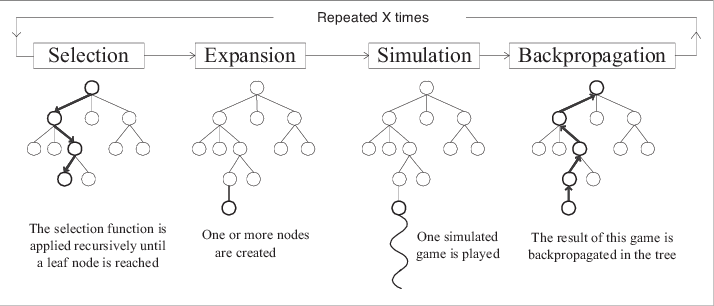
\includegraphics[width=\textwidth]{pictures/MCTSsteps.png}
\end{center}
\caption[MCTS steps]{Steps of the Monte Carlo tree search algorithm \cite{article}}
\label{fig:MCTSsteps}
\end{figure}

\medskip\noindent
The algorithm repeats this four steps until the end condition is met: this can be either a time constraint, a memory constraint or a limit in terms of number of iterations. At this point, the algorithm selects the best action for the root node according to a chosen criteria. Schadd \cite{bestcriteria} describes four
criteria for selecting the winning action, based on the work of
Chaslot et al. \cite{article}:
\begin{itemize}
    \item \textit{max child}: selects the child with the highest reward;
    \item \textit{robust child}: selects the most visited root child;
    \item \textit{max-robust child}: select the root child with both the highest visit count and the highest reward;
    \item \textit{secure child}: select the child which maximizes a lower confidence bound.
\end{itemize}
A MCTS algorithm is thus defined by the mentioned criterium, and by the policies used during the search. In the four steps of the algorithm we can identify four different policies:
\begin{itemize}
    \item \textit{Selection policy}: used to determine the way in which the tree is explored in the selection phase;
    \item \textit{Expansion policy}: used to determine which nodes are created in the expansion phase (usually one or all);
    \item \textit{Simulation policy}: used to determine the rollout behaviour. The usual default policy is a random policy, in which moves are sampled from a uniform distribution among those available in the current state, but often a policy handcrafted for the specific domain can obtain better performance;
    \item \textit{Backpropagation policy}: used to determine how the rewards are propagated in the tree. In the classical version of the method the reward is added to the sum of the rewards of a node and the number of visits is incremented.
\end{itemize}

\medskip\noindent
A general MCTS approach is summarized in Algorithm \ref{GeneralMCTS}. In this algorithm \textit{v\textsubscript{0}} is the root node corresponding to state \textit{s\textsubscript{0}}, \textit{v\textsubscript{l}} is the last node reached during the tree policy stage and corresponds to state \textit{s\textsubscript{l}}, and $\Delta$ is the reward for the terminal state reached by running the default policy from state \textit{s\textsubscript{l}}. The result of the overall search \textit{a}(\texttt{BESTCHILD}(\textit{v\textsubscript{0}})) is the action \textit{a} that leads to the best child of the root node \textit{v\textsubscript{0}}, where the exact definition of “best” is defined by the implementation.

\begin{algorithm}
  \caption[General MCTS approach]{\textbf{General MCTS approach}}\label{GeneralMCTS}
  \begin{algorithmic}
  \Function{MctsSearch}{$\textit{s\textsubscript{0}}$}
    \State create root node \textit{v\textsubscript{0}} with state \textit{s\textsubscript{0}}
    \While{within computational budget}
        \State $\textit{v\textsubscript{l}}\gets \Call{TreePolicy}{v\textsubscript{0}}$
        \State $\Delta\gets \Call{DefaultPolicy}{s(v\textsubscript{l}})$
        \State $\Call{Backup}{v\textsubscript{l}, \Delta}$
    \EndWhile
    \State \Return $\textit{a}(\Call{BestChild}{v\textsubscript{0}})$
    \EndFunction
  \end{algorithmic}
\end{algorithm}

\section{Upper Confidence Bounds for Trees}
Upper Confidence Bounds for Trees (UCT) is a version of the MCTS algorithm that uses UCB1 as a tree policy. The selection of a child node is therefore treated as a multiarmed bandit problem, in which the rewards correspond to random variables with unknown distributions. A child node i is thus selected to maximize
\begin{equation}\label{uctequation} 
UCT = \frac{v_i}{n_i} + C \times \sqrt{\frac{2\ln{n_p}}{n_i}} 
\end{equation}
where $v_i$ is the sum of the rewards obtained in all rollouts that have passed through node i, $n_i$ is number of times the node i (child of p) has been visited, $n_p$ is number of times the current node has been visited and $C$ is a constant used to balance exploration and exploitation. This formula is intrinsically balanced between the exploitation and exploration (represented respectively by the first and second term) as the number of visits of a node $n_i$ increases (inevitably together with $n_p$), the second term decreases, while when another child of the same parent node is visited, only $n_p$ in the numerator increases.
The constant value can be adjusted to favor exploration or exploitation. The value of $C=1$ was shown to ensure the asymptotic optimality of the solution with rewards the range [0,1] \cite{Kocsis2006ImprovedMS}. With rewards outside this range, appropriate values of $C$ could be found by manual tuning or other automated method \cite{Rubinstein1999}. Algorithm \ref{UCTalgorithm} shows the UCT algorithm in pseudocode.

\begin{algorithm}
  \caption[UCT Algorithm]{\textbf{UCT Algorithm}}\label{UCTalgorithm}
  \begin{algorithmic}
  \Function{UctSearch}{$\textit{s\textsubscript{0}}$}
    \State create root node \textit{v\textsubscript{0}} with state \textit{s\textsubscript{0}}
    \While{within computational budget}
        \State $\textit{v\textsubscript{l}}\gets \Call{TreePolicy}{v\textsubscript{0}}$
        \State $\Delta\gets \Call{DefaultPolicy}{s(v\textsubscript{l}})$
        \State $\Call{Backup}{v\textsubscript{l}, \Delta}$
    \EndWhile
    \State \Return $\textit{a}(\Call{BestChild}{v\textsubscript{0}, 0})$
    \EndFunction
    
    \Function{TreePolicy}{$v$}
    \While{\textit{v} is nonterminal}
        \If{\textit{v} not fully expanded}
        \State \Return $\Call{Expand}{v}$
        \EndIf
        \State \textbf{else}
        \State \hspace{\algorithmicindent}$v\gets \Call{BestChild}{v, C\textsubscript{p}}$
    \EndWhile
    \State \Return $v$
    \EndFunction
    
    \Function{Expand}{$v$}
    \State choose \textit{a} $\in$ untried actions from \textit{A}(\textit{s}(\textit{v}))
    \State add a new child \textit{v'} to \textit{v}
    \State \hspace{\algorithmicindent} with \textit{s}(\textit{v'}) = \textit{f}(\textit{s}(\textit{v}), \textit{a})
    \State \hspace{\algorithmicindent} and \textit{a}(\textit{v'}) = \textit{a}
    \State \Return \textit{v'}
    \EndFunction
    
    \Function{BestChild}{$v, c$}
    \State \Return $\argmax\limits_{v' \in \,children\,of\,v} \frac{Q(v')}{N(v')} + c \times \sqrt{\frac{2\ln{N(v)}}{N(v')}}$
    \EndFunction
    
    \Function{DefaulPolicy}{$s$}
    \While{\textit{s} is non-terminal}
        \State choose \textit{a} $\in$ \textit{A}(\textit{s}) uniformly at random
        \State $s\gets f(s, a)$
    \EndWhile
    \State \Return reward for state \textit{s}
    \EndFunction
    
    \Function{Backup}{$v, \Delta$}
    \While{\textit{v} is non null}
        \State $N(v)\gets N(v) + 1$
        \State $Q(v)\gets Q(v) + \Delta(v, p)$
        \State $v\gets$ parent of $v$
    \EndWhile
    \EndFunction
  \end{algorithmic}
\end{algorithm}

\medskip\noindent
Each node \textit{v} contains information about: the associated state \textit{s}(\textit{v}), the outgoing action \textit{a}(\textit{v}), the total simulation reward \textit{Q}(\textit{v}) and the visit count \textit{N}(\textit{v}). To have a more efficient usage of memory, the associated state \textit{s}(\textit{v}) is recomputed as \texttt{TREEPOLICY} descends the tree, instead of storing it for each node. The term $\Delta(v,p)$ in function \texttt{BACKUP} indicates the component of the reward vector $\Delta$ associated with the current player \textit{p} at node \textit{v}. The return value of the overall search is given by \textit{a}(\texttt{BESTCHILD}(\textit{v\textsubscript{0}})), that is the action \textit{a} associated to the child which has the highest reward, due to the fact that the exploration parameter \textit{c} is set to 0 for the final call of this function on the root node \textit{v\textsubscript{0}}.

\section{Characteristics}
MCTS is a popular choice of algorithm for a variety of domains due to three main characteristics:
\begin{enumerate}
    \item \textit{Analytic}: MCTS does not require any domain-specific knowledge, it is sufficient to know only its legal moves and end conditions. This makes it applicable to any domain that can be modeled using a tree. However, in its basic version, MCTS can have low performance and some domain-specific knowledge can be included in order to significantly improve the speed of the algorithm;
    \item \textit{Anytime}: MCTS backpropagates the outcome at the end of every iteration, so the whole tree is immediately updated with the last calculated rewards and visits counts. This allows the algorithm to stop and return the current best root action at any moment in time. Allowing the algorithm to run for extra iterations often improves the result;
    \item \textit{Asymmetric}: The tree policy allows the algorithm to use more computational resources on the most promising nodes of the tree, leading to an asymmetric growth of it over time. This makes the tree adapt to the topology of the search space leading to a better understanding about the game itself and making MCTS suitable for games with high branching factor.
\end{enumerate}

\section{MCTS Enhancements}
A huge number of enhancements have been proposed for the core MCTS algorithm in order to improve performance, including modifications of the tree policy, the default policy and other more general modifications related to the backpropagation step and parallelization as described in Cameron et al. work \cite{journals/tciaig/BrownePWLCRTPSC12}. These enhancements can generally be divided into two categories: \textit{Domain independent} enhancements that do not require any prior knowledge about the domain in order to be applied in it; \textit{Domain dependent} enhancements that are specific to particular domains. A more specific categorization can be done considering the used approach.

\subsubsection{Bandit-Based Enhancements}
This approach modifies the bandit-based method used for node selection in the tree policy. For this kind of enhancements plenty of different upper confidence bounds have been proposed, often improving bounds or performances in particular circumstances.

\subsubsection{Selection Enhancements}
This approach modify the tree policy in order to change how MCTS explores the search tree. The basic idea of selection is to assign a numeric score to each action in order to balance exploration with exploitation, so these enhancements influence this score using some domain knowledge in order to bias the search toward the most promising area and make use of different kind of reward estimation.

\subsubsection{All Moves As First (AMAF)}
This approach modifies how node statistics are updated. The basic idea is to update statistics for all action that are selected during a rollout as if they were the first action applied. The AMAF algorithm treats all moves played during selection and rollout steps as if they were played on a previous selection step, meaning that the reward estimate for an action \textit{a} from a state \textit{s} is updated whenever \textit{a} occurs during a playout, even if \textit{a} was not the actual move chosen from \textit{s}.

\subsubsection{Game-Theoretic Enhancements}
This approach uses the known game-theoretic value of a state to improve reward estimates for other non-terminal nodes backpropagating it up the tree.

\subsubsection{Move Pruning}
This approach applies the pruning technique, already used with \textit{minimax}, in order to eliminate obviously poor choices and allow the search to focus more resources on the better ones.

\subsubsection{Simulation Enhancements}
This approach modifies the default simulation policy for MCTS which select randomly among the available actions, trying to obtain more realistic simulations by incorporating domain knowledge into the playouts.

\subsubsection{Backpropagation Enhancements}
This approach modifies the backpropagation step involving special node updates.

\subsubsection{Parallelization Enhancements}
This approach exploit the independent nature of each simulation in MCTS to introduce parallization. More simulations can be performed in a given amount of time and the wide availability of multicore processors can be exploited. However, parallelization raises issues such as the combination of results from different sources in a single search tree, and the synchronization of threads of different speeds over a network.

\section{MCTS for puzzles}\label{sec:spmcts}
UCT was initially proposed for two-player games, therefore --- as in minimax and other adversarial search algorithms --- some of its characteristics were based on the assumption that there was a second player with the goal of minimizing our reward. Schadd et al. \cite{DBLP:journals/kbs/SchaddWTU12} presented a variant called \textit{Single-Player Monte-Carlo Tree Search} (SP-MCTS) in which they exploit some properties of single-player games to increase the effectiveness of MCTS. The core mechanism of SP-MCTS is the same as in UCT. One of the new ideas introduced is a variation the selection strategy, which aims to maximize the following formula:
\begin{equation}\label{spmctsequation}
    SP-UCT = \frac{v_i}{n_i} + C \times \sqrt{\frac{2\ln{n_p}}{n_i}} +\sqrt{\frac{\sum{v_i^2} - n_i \times (\frac{v_i}{n_i})^2 + D}{n_i}}
\end{equation} 
where the first two terms represent the UCT formula \ref{uctequation}, while the newly added term represents possible deviations in the child node scores. Using the same notation used in the UCT formula, $\sum{v_i^2}$ is the sum of squared rewards obtained by rollouts that have transited through node $n_i$, $n_i \times (\frac{v_i}{n_i})^2$ is the expected squared reward, $D$ is a large constant used to ensure that rarely explored nodes are considered promising.

\medskip\noindent
One of the aspects in which puzzles can differ from zero-sum two-player games is the range of values for the reward. While in two-player games the outcome is usually defined as \{0, $\frac{1}{2}$, 1\} or \{-1, 0, 1\} for loss, draw or win, in puzzles where the goal is to maximize the score the reward can vary greatly in range. Keeping in mind that \cite{DBLP:journals/kbs/SchaddWTU12} chose Samegame as a case study (which has a score in the order of thousands), the third term of the formula was specifically designed to take advantage of the score variation. Another major difference from two-player games is the absence of an opponent. The consequence is that if the game is deterministic there is no uncertainty given by the opponent choices. This leads to the second variation introduced in SP-MCTS: the method to choose the root action at the end of the search is not one of the four mentioned in Section \ref{mctsalgorithm} which generally aim towards the maximization of the winning probability, but instead the selected action is the one that belongs to the path which maximizes the top score. In order to employ this policy and to evaluate equation \ref{spmctsequation} the backpropagation policy was slightly modified to store in the nodes additional information like the total squared rewards and the top score. The best solution, i.e. the one with the highest score, was also stored throughout the search to ensure that the final result is the best among all rollouts executed.

\medskip\noindent
Schadd et al. \cite{DBLP:journals/kbs/SchaddWTU12} also applied a single-threaded version of root parallelization \cite{10.1007/978-3-540-87608-3_6} called \textit{Randomized Restarts} in which the search is repeated multiple times with different random seeds to avoid getting caught in local optima.
They used the \textit{Cross Entropy Method} \cite{Rubinstein1999} to tune the parameters and managed to obtain a score of 78012 in a standardized Samegame test set.

\subsection{Samegame}\label{sec:samegame}
Samegame is a fully observable deterministic single player game invented by Kuniaki Moribe under the name \textit{ChainShot!} in 1985.  In 1992 Eiji Fukumoto ported the game to Unix with a slight variation in settings calling it Samegame. Samegame is a tile-matching game and numerous variations of the game have been developed over the years.

\subsubsection{Rules}
Samegame is played on an $n\times m$ grid containing randomly arranged blocks of $k$ different colors. The goal of the game is to obtain the highest score by removing groups of blocks. At every move, the player can remove a group of two or more orthogonally adjacent blocks of the same color. Once a block has been removed, all blocks above it in the same column will slide down until there are no holes left, as if they were subject to gravity, as shown in Figure \ref{fig:samegame_b}. Once an entire column is removed, all columns on its right will slide to the left until there are no empty columns left, as shown in Figure \ref{fig:samegame_c}.

\begin{figure}[ht]
\label{fig:samegameexample}
\centering
\subfigure[Playing move (C,3)]{
\label{fig:samegame_a}
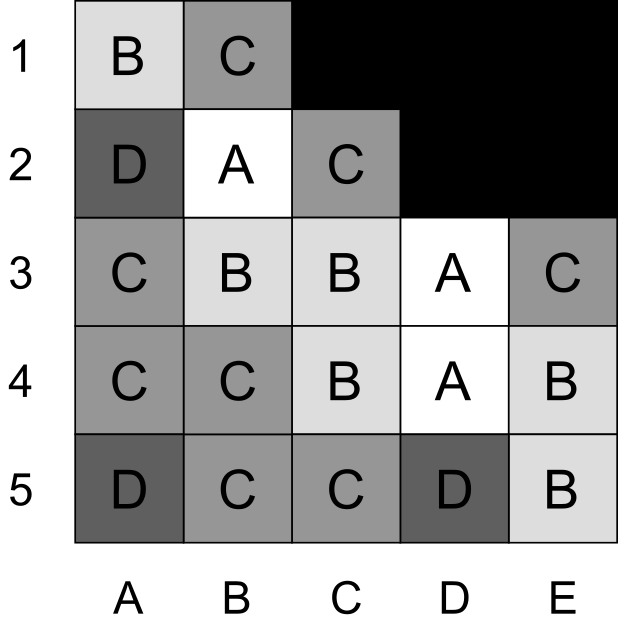
\includegraphics[width=0.28\linewidth]{pictures/samegame_a.png}}
\quad
\subfigure[Playing move (C,4)]{
\label{fig:samegame_b}
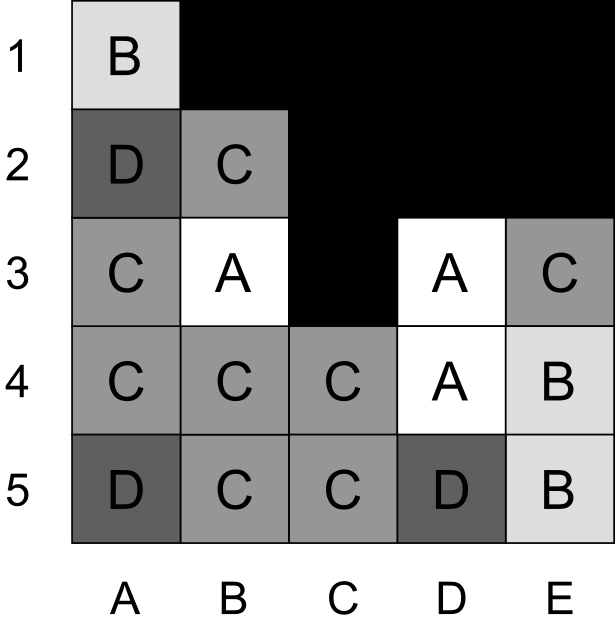
\includegraphics[width=0.28\linewidth]{pictures/samegame_b.png}}
\quad
\subfigure[Result]{
\label{fig:samegame_c}
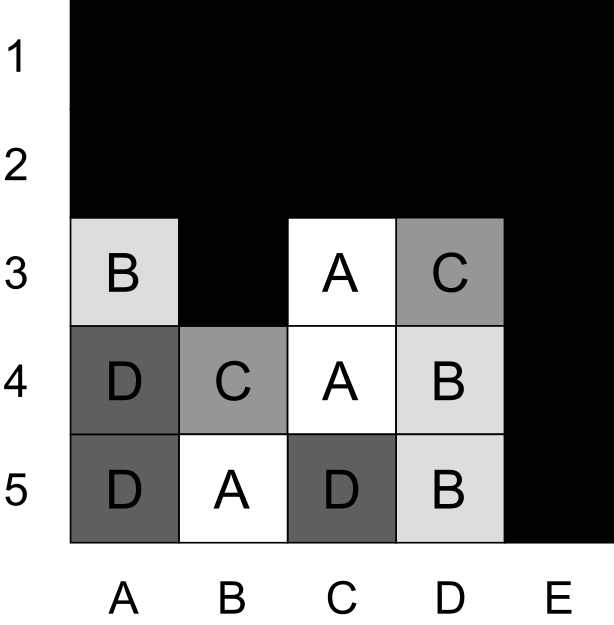
\includegraphics[width=0.28\linewidth]{pictures/samegame_c.png}}
\caption[Move sequence example]{Move sequence example \cite{DBLP:journals/kbs/SchaddWTU12}}
\end{figure}

\medskip\noindent
Points are rewarded for each action according to the formula $(n-2)^2$, where $n$ is the number of blocks removed with the current action. The game is over when either the player has cleared the board, leaving no blocks behind, or there are no more legal moves left, meaning that there are no two blocks with the same color are adjacent to each other.\\
Final points are awarded or subtracted based on the above end game condition: 
\begin{itemize}
    \item If the player was able to clear the board: A bonus of 1000 points is awarded.
    \item If the player was unable to clear the board: Points are subtracted using the formula $\sum{(n_i-2)^2}$ where $n_i$ is the number of blocks of the same color still on the board.
\end{itemize}
The standard game configuration is a $15\times 15$ board with $5$ colors. Given the scoring system, the maximum theoretical achievable score is $(n\times m-2)^2 +1000$, with $n$ and $m$ being rows and columns. With the standard configuration this results in a total of 49829. This is only obtainable if the initial configuration contains only a single color, requiring that no constraint on the minimum number of colors present are applied. If we consider enforcing the presence of all 5 colors, the maximum score becomes 48861. However, the actual score for a randomly generated board is rarely higher than 6000 points. On the 20 levels standard test set used in most researches \cite{DBLP:journals/kbs/SchaddWTU12} \cite{Cazenave2009} \cite{IJCAI113358}, the average score of the best algorithm is 4392.1 \cite{highscore}.

\medskip\noindent
The same mechanics can be found in other games, with the only difference often being the scoring formula. In \textit{Clickomania!} for example the objective is minimizing the number of blocks remaining, thus clearing the board represent the top score. In \textit{Jawbreaker}, a the Samegame porting for Microsoft Windows Mobile 2003, the formula used is $n(n-1)$, while in the Windows 3.1 porting the game is still called Samegame, but it computes the score as $n^2-3n+4$.

\subsubsection{Complexity}
A good estimator for the complexity of a game is the game-tree complexity, that represents the number of leaf nodes in the search tree and can be approximated by $b^d$, where $b$ is the average branching factor and $d$ is the average game length. In Samegame the player can choose a block as a move and in a $15\times 15$ board that would lead to an initial branching factor of 225. In reality, all moves in the same block group are equivalent so the actual branching factor is normally smaller. It also generally decreases as the game progresses. Schadd et al. \cite{DBLP:journals/kbs/SchaddWTU12} calculated the average game length and the average branching factor over 250 different configurations, and obtained $d=62.2$ and $b=21.1$, resulting in a game-tree complexity of $10^{82}$.Another estimator for the complexity can be the state-space complexity, which is the total number of legal board configurations reachable from the initial state. In the case of Samegame, it can be computed as $C^m$ where $m$ is the number of columns and $C$ is the number of possible configurations of a single column, obtained as $C=\sum_{i=0}^n{k^i}$, where n is the number of rows and k is the number of different colors. With $n=15$, $m=15$ and $k=5$ we can obtain a state-space complexity of $10^{159}$. Furthermore, Samegame has been proven to be at least of complexity class NP-complete \cite{DBLP:journals/kbs/SchaddWTU12}.

\medskip\noindent
In addition to the sheer values of game-tree and state-space complexity - that render uninformed search methods unfeasible - it's very hard to find a reliable admissible heuristic, given that with every move, new block groups can be created and existing groups can be dismantled.
\chapter{Our Approach}
\label{proposedsolution}
In this chapter we present our solution to the puzzle solving problem. The proposed solution takes into account IDA*, MCTS and some enhancements of standard versions of these algorithms. We describe the enhancements implemented and added to the basic algorithms and to Sokoban. First, we describe the implemented IDA* optimizations; next we describe optimizations for the MCTS algorithm. The enhancements are either domain independent, which can be applied to each algorithm and to both the considered domains, or domain dependent, specific for the different domains.

\section{IDA* optimizations}
The performance of IDA* is strongly tied to the quality of the heuristic evaluation, however there are techniques that can improve the results under certain conditions by reducing the size of the search tree or the order in which nodes are explored.

\subsection{Transposition Tables}
Transposition tables are a data structure that keeps track of the visited states in order to reduce the branching factor of the game tree. The assumption at the base of the use of transposition tables is that the same state can be reached through different paths. When this assumption holds, transposition tables can be used to avoid cycles during the search by expanding only nodes that represent a state that has not yet been visited. In addition to cycles avoidance, we can use transposition tables to prune sub-trees according to the outcome of previous searches.

\medskip\noindent
A transposition table requires: an entry, a record that represent the state and data relevant to the search; an hash table, the actual table that holds an entry in each cell.
\begin{figure}[ht]
\centering
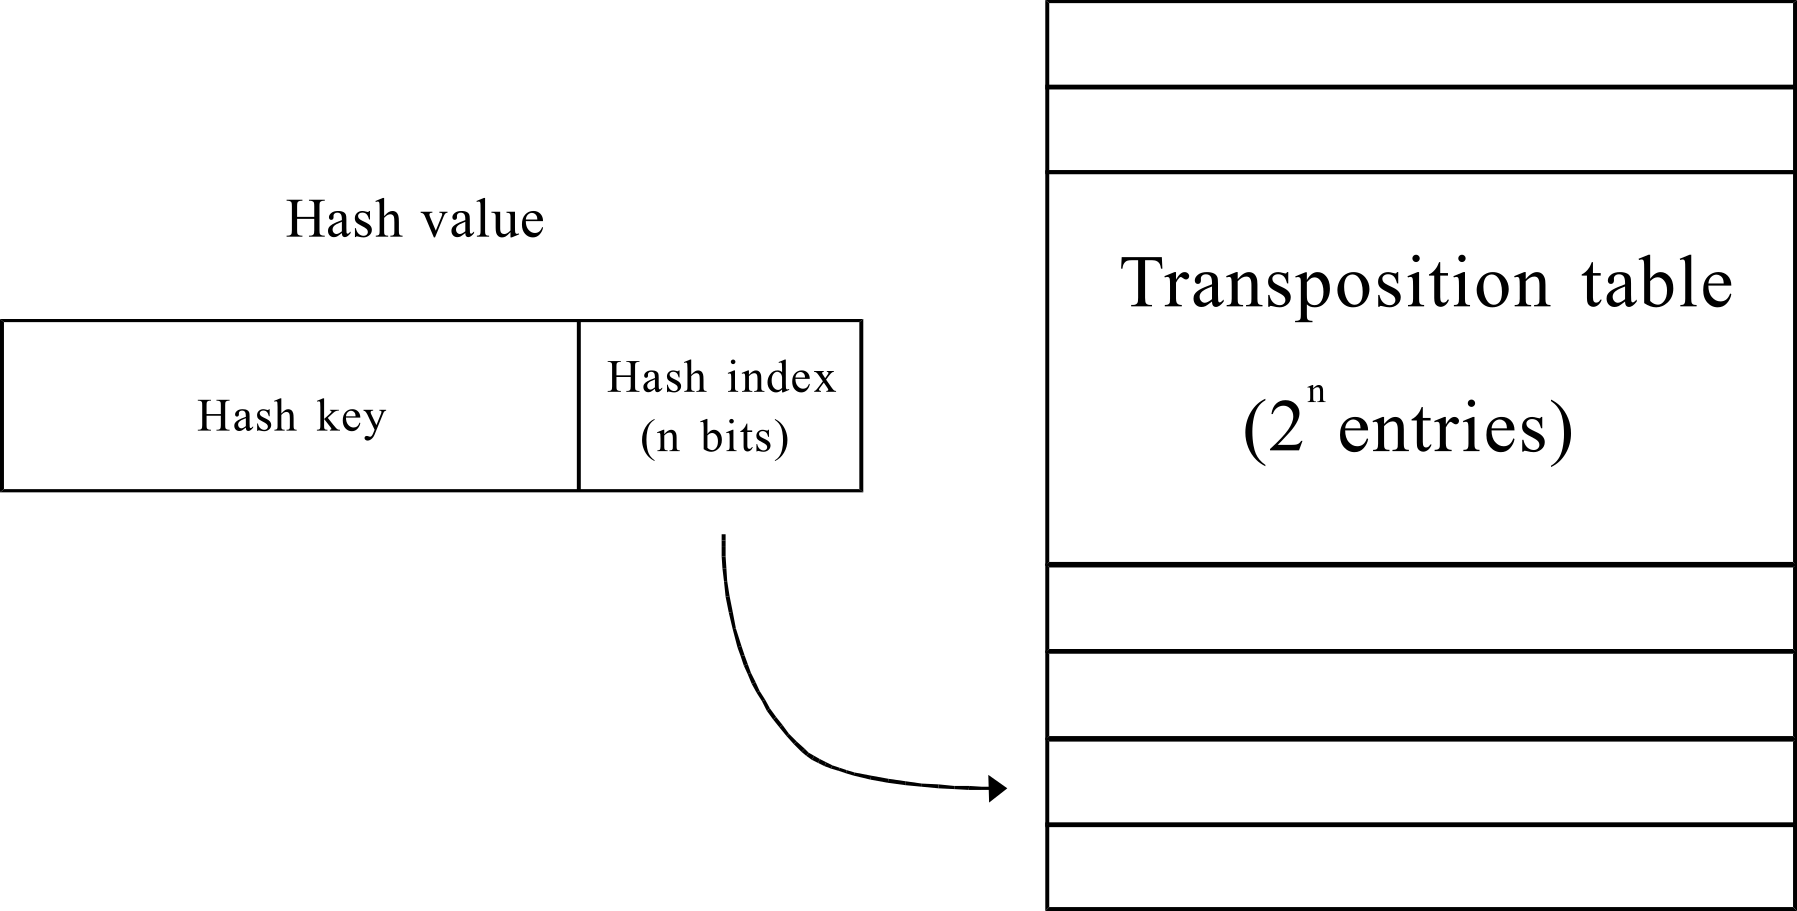
\includegraphics[width=0.6\linewidth]{pictures/TranspositionTable.png}
\caption[Hash Table]{Hash Table \cite{transpositiontables}}
\label{fig:transpositiontable}
\end{figure}

\medskip\noindent
Figure \ref{fig:transpositiontable} shows the typical usage of transposition tables. The hash value is computed through an hash function specifically built for the domain we are considering. The perfect hash function should be built in such a way that two states that should be considered different for the search purpose have different hash values, while two state that should be considered equivalent have the same hash value. Once computed, the \textit{hash index}, a portion of the hash value of a state, is used as an index to access the table, while either the remaining portion of the hash called \textit{hash key}, or the full hash value is stored inside the table to handle collisions that might happen between different states that map onto the same index.
Therefore, the table entry should contain the either the hash key or the hash value, along with all data that is relevant to the search. In the case of IDA*, this data include
\begin{itemize}
    \item \textit{Score}: the heuristic value obtained in previous visit through the state. When the state is first added to the transposition table, the score should be its heuristic value. Once the sub-tree that starts from the state has been completely explored up to the threshold, the score oh the state should be updated with the score obtained further along the search, since it's supposed to be more accurate. In the case of IDA*, it's computed as the minimum value among the successors of the current node.
    \item \textit{Depth}: the relative depth of the explored sub-tree. This represents how deep the tree has been explored, starting from the current state. In the context of IDA*, the depth can be computed as $threshold-g$, where $threshold$ is the threshold of the current iteration and $g$ is the cost of the path from the root state to the current state.
    \item \textit{Visited}: a flag that represent whether the entry is part of the current path or it has been added in a previous search. This allows us to discern between cycle avoidance and tree pruning.
\end{itemize}

\medskip\noindent
In an ideal setting, the transposition table size would be enough to hold every state visited during the search. In real applications, such as Samegame and Sokoban, with large branching factors, we limit the size of the table as shown in Figure \ref{fig:transpositiontable}. A replacement scheme represent the policy used to handle conflicts. The replacement scheme defines whether upon collision, the entry contained in the table should be kept or should be replaced with the new entry. Breuker \cite{transpositiontables} examined several different replacement schemes based on different concepts:
\begin{itemize}
    \item \textit{Deep}: The entry with the largest depth is kept in the table. The rationale behind this scheme is that the sub-tree associated to an entry with a great depth contains more nodes than the lower depth one, thus containing more accurate information and saving more work in case of pruning.
    \item \textit{New}: The newest entry is kept in the tree. This scheme is based on the observation that most transposition occur in local sub-trees, implying that keeping most recent nodes in the transposition table allows us to prune more often.
    \item \textit{Old}: The oldest entry is kept in the tree. No replacement occurs. The author included this scheme only for the sake of completeness.
    \item \textit{Big}: The entry with the largest amount of nodes in the sub-tree is kept in memory. This is similar to the Deep scheme and might perform better when the depth is not a good estimator of the size of the sub-tree, but requires to keep in the entry also the number of nodes, effectively reducing the number of entry that can be stored in the table.
    \item \textit{Two-Level}: The transposition table is organized in two levels and the replacement scheme is combined with one of the above. The the main replacement scheme is applied with the selected entry stored in the first level of the table, while the entry that would normally be discarded is stored on the second level. When retrieving the entry, the second table is used only if there's no match in the first table. This scheme allows us to store both more recent (to increase the number of hits) and more informative entries (to prune large sub-trees). Note however that keeping two tables imply that the number of entry stored for each table is halved.
\end{itemize}
Breuker \cite{transpositiontables} results showed that the two-level replacement scheme obtains the highest reduction in number of explored nodes, with its Big combination having a slight edge over the Deep one. We decided however to follow Junghanns et al. \cite{Junghanns99pushingthe} example and implemented a two-level transposition table based on depth, since it lends itself well for use with IDA*, as depth can be computed before actually exploring the sub-tree, as mentioned earlier.

\medskip\noindent
As we already mentioned, the effect of transposition tables on IDA* is two-fold: cycles avoidance and tree pruning.
In practice, the search explores a new node, it first checks the transposition table for an entry with the same state. If one is found and its depth is greater than the current estimated depth, the node is not explored further and its value is returned as the score of the entry. Otherwise, the a new entry is stored and the search continues among the successors (Algorithm \ref{alg:idastar}), with the exception that only child nodes that do not appear as visited are explored.

\subsection{Move ordering}
IDA* explores in a depth first manner, so if the algorithm explores promising nodes first, it will find a solution faster. Following this idea, move ordering sorts the available moves before expansion according to a certain criterion. This criterion can be domain dependent, as in \cite{Junghanns99pushingthe}, or domain independent, as in \cite{DBLP:journals/pami/ReinefeldM94}. We decided to implement move ordering with a domain independent ordering criterion by sorting the moves according to the heuristic evaluation of the resulting state.
\medskip\noindent
Since in IDA* all iterations except for the last one perform a complete search, the only contribution of move ordering is visible on the last iteration, but since that is the largest one by number of nodes, if the solution is found in an earlier sub-tree it may reduce execution time by a significant amount.

\section{MCTS configuration}\label{rewardtype}
To identify a specific MCTS configuration we need to define simulation policies and the rewards used. We defined four different reward types for Sokoban:

\begin{enumerate}
    \item \textit{R0}: 1 if the state represents a solved level, 0 otherwise.
    \item \textit{Boxes}: the reward is the same as the one used by \cite{DBLP:journals/corr/WeberRRBGRBVHLP17} and is computed as
    \begin{equation}
        r = 0.1\times steps + b_{ON} - b_{OFF} + solved 
    \end{equation}where $steps$ is the number of pushes executed, $b_{ON}$ is the number of times a box has been pushed on a goal, $b_{OFF}$ is the number of times a box has been pushed off a goal and $solved$ is 10 if the level is solved, 0 otherwise.
    \item \textit{InverseBM}: $1/\sqrt{BM}$, where $BM$ is the \textit{minimum cost perfect matching on a complete bipartite graph}, i.e. the minimum sum of the distances from each box to its designated goal. $BM$ is the heuristic evaluation used by \cite{Junghanns99pushingthe}. This reward has the advantage of having values in the range \{0,1\}.
    \item \textit{NegativeBM}: $-BM$. This reward has values in the range \{$-\infty$,0\}, but has the advantage of the linearity of the reward.
\end{enumerate}

\medskip\noindent
We tested different simulation policies:
\begin{itemize}
    \item \textit{random}: selects a random action among those available in the current state.
    \item \textit{$\epsilon$-greedy}: selects a random action with probability $\epsilon$ or the action that maximizes the reward of the resulting state with probability $1-\epsilon$.
    \item \textit{$\epsilon$-IDA*}: selects a random action with probability $\epsilon$ or -- with probability $(1-\epsilon)$ -- perform an IDA* search with a limited number of nodes and return the first action of the path that leads to the state with the lowest heuristic value. For this policy we tested different configurations in terms of number of IDA* nodes and MCTS iterations.
\end{itemize}
For the backpropagation policy, in addition to the usual sum of rewards and number of visits we stored the maximum score, the sum of the squared rewards and the sum of rewards and visits for the RAVE optimization (Section \ref{sec:rave}). The winning action is the one with the highest maximum score.

\section{MCTS optimizations}
Standard version of the core MCTS algorithm can be applied to various domains due to its main characteristic of not requiring domain-specific knowledge, but when it is needed to compare it - in a specific domain - with another artificial intelligence modified in order to have good performance in such domain, it can work not so well. In order to achieve better results in this kind of comparison, we need to modify the standard algorithm introducing some enhancements in order to improve performance.

\medskip\noindent
In the proposed solution all enhancements are domain independent, so can be applied to any domain without prior knowledge about it, this choice is done in order to have a unique optimized MCTS algorithm that can be used in each game considered in this work without the need of any change due to some specific knowledge.

\subsection{Object Pooling}
The Object Pool pattern is a software creational design pattern used to improve memory usage and performance. This pattern uses a set of initialized objects kept ready to use --- also called ``pool'' --- rather than allocating and destroying them on demand. In order to use this pool, it is possible to require an object from it and then perform operations on the returned object. When the object is not used anymore, it can be returned to the pool, in order to have the possibility to use it again later, rather than destroying it; this can be done manually or automatically.

\medskip\noindent
The MCTS algorithm can create a large number of objects that are particularly expensive to instantiate and each object is only needed for a short period of time; so this can have a huge impact on performance. Using Object Pool pattern it is possible to create a set of objects that may be reused. When a new object is needed, it is requested from the pool. If a previously prepared object is available it is returned immediately, avoiding the instantiation cost. If no objects are present in the pool, a new item is created and returned. When the object has been used and is no longer needed, it is returned to the pool, allowing it to be used again in the future without repeating the computationally expensive instantiation process. The same pool can also be used in different consecutive run of the algorithm leading to a huge benefit in terms of memory performance.

\subsection{Node Recycling}
This optimization is a memory enhancement that can bring significant performance benefits. Considering the structure of the core MCTS algorithm, performing more iterations causes a huge increase of memory used by the algorithm, due to the fact that MCTS usually add a new node on each iteration. So as the number of iterations --- performed by the MCTS algorithm --- increase, the memory usage of the algorithm is bounded only by the size of the game tree.

\medskip\noindent
Powley et al. \cite{AIIDE1715856} present a study of different memory bounding techniques for the MCTS algorithm. The technique called \textit{Node Recycling} is used in the proposed solution. Node Recycling method aims to throw away the policy information, learned by MCTS, that is least relevant to the search preserving as much useful information as possible in the remaining tree.

\medskip\noindent
The basic idea of this technique is to remove nodes coming from unpromising areas of the tree and recycle the freed memory to build more promising ones. This approach is due to the fact that the behaviour of MCTS algorithm is to repeatedly visit the most promising areas of the search tree and, at the same time, decrease the frequency of exploration of less promising areas. Thus it make sense to recycle these areas of the tree that have not recently been accessed, as they have a low priority for being exploited.

\medskip\noindent
The overall idea of Node Recycling is to allocate a fixed pool of nodes of size determined by a memory budget, rather than creating a new node upon each expansion step of the algorithm. These nodes are used until the pool is exhausted, after that the recycling process begin. The node to be recycled is the leaf node whose statistics have least recently been accessed, in other words the node for which the UCB1 score has least recently been calculated.

\medskip\noindent
The implementation of the Node Recycling technique is done trying to not significantly increase the amount of execution time taken by each iteration of the MCTS algorithm. In order to find the least recently accessed leaf node without scanning the whole tree, a queue structure is used. Nodes of the tree are managed using a least recently used (LRU) cache implemented as a first-in first-out (FIFO) queue. During a MCTS iteration, when a node is accessed it is removed from its current position in the queue and it is pushed to the back. When the memory budget is reached (the pool of nodes is empty), the node on top of the queue is recycled.

\subsection{SP-MCTS UCB}
This optimization is a bandit-based enhancement suggested by Schadd et al. \cite{DBLP:journals/kbs/SchaddWTU12} to improve the selection step of the core MCTS algorithm modifying the standard UCT with formula \ref{spmctsequation}. A description of the method can be found in Section \ref{sec:spmcts}.
%At the selection of node \textit{p} with children \textit{i}, the strategy chooses the move, which maximizes the following formula
%\begin{equation}
%    v\textsubscript{i} + C \times \sqrt{\frac{2\ln{n\textsubscript{p}}}{n\textsubscript{i}}} + \sqrt{\frac{\sum{r\textsuperscript{2}} - n\textsubscript{i} \times v\textsubscript{i}\textsuperscript{2} + D}{n\textsubscript{i}}}
%\end{equation}
%The first two terms constitute the original UCT formula. It uses \textit{n\textsubscript{i}} as the number of times that node \textit{i} was visited, where \textit{i} denotes a child and \textit{p} the parent to give an upper confidence bound for the average game value \textit{v\textsubscript{i}}. For puzzles in this formula a third term is added and represents a possible deviation of the child node. It contains the sum of the squared results ($\sum{ r\textsuperscript{2}}$) so far achieved at the child node, corrected by the expected results $n\textsubscript{i} \times v\textsubscript{i}\textsuperscript{2}$. An high constant D is added to ensure that nodes, which have been rarely explored, are considered promising. As this deviation term is not domain specific, it may also be beneficial in other domains where the variation on the scores is an important feature (e.g., puzzles with the aim to score points).

\subsection{UCB1-Tuned}
This optimization is a bandit-based enhancement suggested by Auer et al. \cite{Auer2002} to tune more finely the bounds of UCB1. This approach uses formula \ref{ucb1variance} as upper confidence bound for the variance of the arm \textit{j} in a multiarmed bandit problem.

\begin{equation}\label{ucb1variance}
    V\textsubscript{j}(s) = (\frac{1}{2}\sum\limits_{\tau=1}^{s} {X^{2}_{j,\tau}}) - \overline{X}^{2}\textsubscript{j,s} + \sqrt{\frac{2\ln{t}}{s}}
\end{equation}
This means that arm \textit{j}, that has been played \textit{s} times during the first \textit{t} plays, has a variance that is at most the sample variance plus $\sqrt{\frac{2\ln{t}}{s}}$ \cite{Auer2002}. Then, the upper confidence bound $\sqrt{\frac{2\ln{n}}{n\textsubscript{j}}}$ of UCB1 is replaced with formula \ref{ucb1tuned}.

\begin{equation}\label{ucb1tuned}
    \sqrt{\frac{\ln{n}}{n\textsubscript{j}}\min\left\{\frac{1}{4}, V\textsubscript{j}(n\textsubscript{j})\right\}}
\end{equation}

\subsection{Rapid Action Value Estimation (RAVE)}\label{sec:rave}
This optimization is an All-Moves-As-First enhancement that combine the standard UCT score for each node with an AMAF score \cite{conf/icai/HelmboldP09}.
Figure \ref{fig:AMAFheuristic} shows the AMAF heuristics in action on a simple situation. UCT is used to select actions during selection step of the core MCTS algorithm, then the simulation step plays some action leading to a terminal state. The basic idea of AMAF heuristic is that UCT could have also selected the simulated moves during the selection step as alternatives. Since these moves were used during the simulation, their corresponding nodes in the tree have their reward/visit count updated by the AMAF algorithm. Nodes that receive the extra AMAF update during backpropagation are marked with an asterisk (*).
\begin{figure}[ht]
\begin{center}
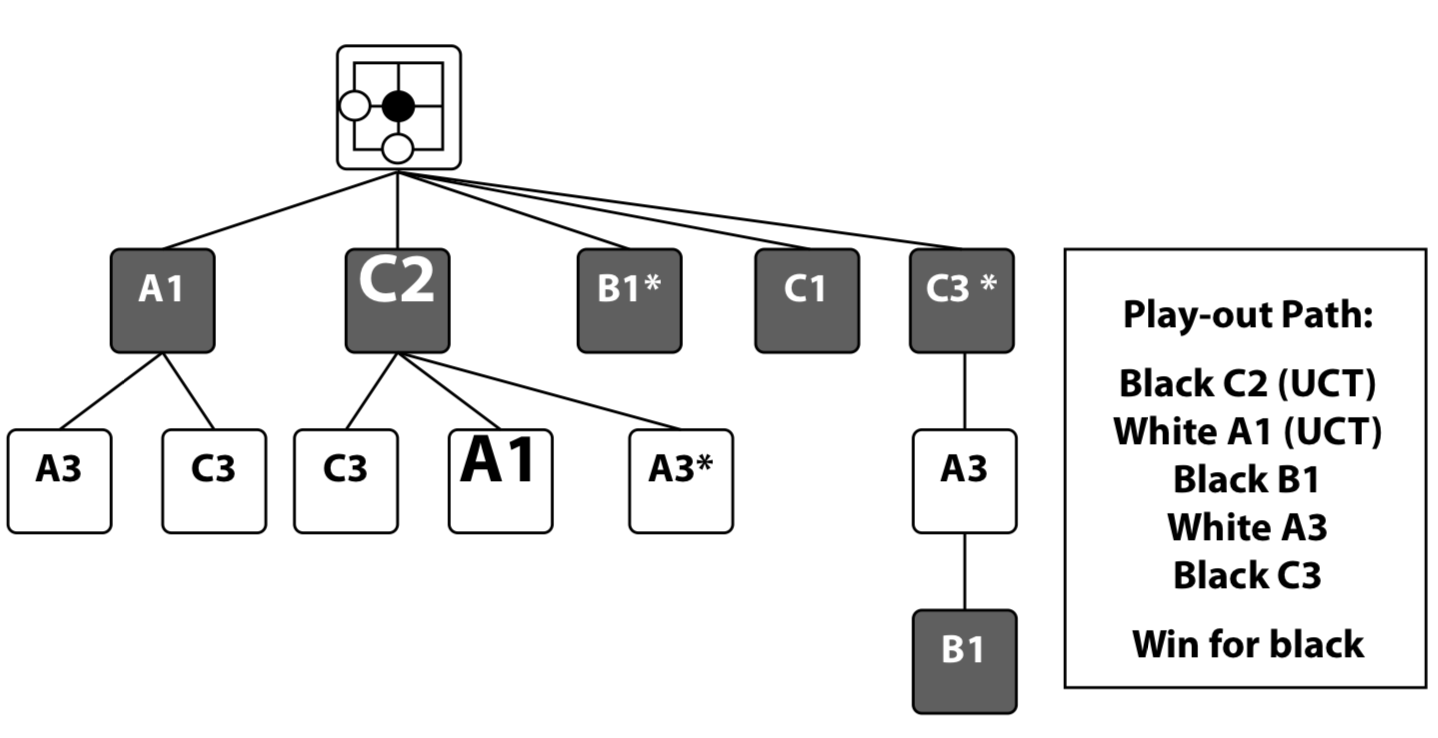
\includegraphics[width=\textwidth]{pictures/AMAF.png}
\end{center}
\caption[AMAF heuristic]{AMAF heuristic \cite{conf/icai/HelmboldP09}}
\label{fig:AMAFheuristic}
\end{figure}
In order to have both values, a separate count of rewards and visits for each type of update is maintained. So the total score of an action is expressed as

\begin{equation}
    \alpha A + (1 - \alpha) U
\end{equation}
where U represent the standard UCT score and A represent the AMAF score.
The value of $\alpha$ used at each node decrease with each visit and it is computed, supplying a fixed positive integer $V>0$, after \textit{n} visit as \cite{conf/icai/HelmboldP09}

\begin{equation}
    \max \left\{0,\frac{V - v(n)}{V}\right\}
\end{equation}
where parameter \textit{V} represent the maximum value of visits a node can have in order to use the RAVE values to correct the UCT score; when a node is visited more times than the value expressed by \textit{V}, RAVE values are not being used at all. With this approach exploited areas of the tree will use the accurate statistics more that unexplored areas of the tree.

\subsection{Node Elimination}
In addition to known enhancements we propose a new method to improve MCTS performance in domains with many early terminal states. One such domain is Sokoban, in which earlier deadlock detection can significantly reduce the search space. The idea behind \textit{Node Elimination} is based on the observation that MCTS often repeatedly selected nodes that would lead to a deadlock inside the tree. This was caused by the constraints posed by the problem itself and we will therefore use Sokoban to illustrate the concept of Node Elimination.

\medskip\noindent
In a Sokoban search, every rollout can end in either a solved state or a deadlock. With deadlocks being far more likely in non trivial levels, penalizing the reward of every rollout that terminated in a deadlock would not be beneficial to the search, since the hard part is not minimizing the cost to the solution but actually finding the solution. Furthermore, the length of the rollout does not give any insight on the quality of the rollout, since the move that originally caused a deadlock might have been executed far before the deadlock was finally detected. This lead to nodes close to the root being selected many times despite representing a deadlock state, wasting search resources. The solution we propose to this kind of situation is a recursive Node Elimination starting from terminal states.

\medskip\noindent
During the backpropagation phase we remove from the tree all nodes in the current path that have no children and no untried moves. Terminal nodes are therefore directly eliminated (as they never have untried moves), effectively removing all deadlocks from the tree. When a node is eliminated it's also removed from its parent's list of children, therefore if every child of a node is a deadlock, that node is removed too. This goes on recursively, removing dead sub-trees that have already been fully explored. The elimination process is illustrated in figure \ref{fig:nodeelimination}.
\begin{figure}[ht]
    \centering
    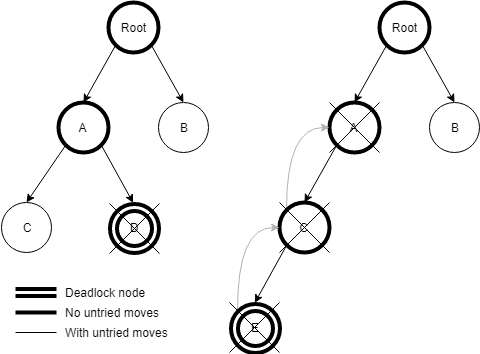
\includegraphics[width=0.9\linewidth]{pictures/NodeElimination.png}
        \caption[Node elimination]{Node elimination:\\
            Simple Node Elimination (left): only node D can be removed because node A still has children.
             Recursive Node Elimination (right): node C is expanded into terminal node E and --- after the 0-length rollout --- nodes E, C and A can be removed because once one is removed, its parent is left with no children and no untried moves.}
    \label{fig:nodeelimination}
\end{figure}
Node Elimination was also combined with Node Recycling by removing eliminated nodes from the node pool.

\medskip\noindent
While in most two-player games, revisiting the same terminal nodes can be beneficial to the accuracy of the evaluation of the best move, in single player games the only required information is the top score achieved among all rollouts. Therefore, once a path has been fully explored it's no longer needed and can be ignored for the rest of the search. In the context of puzzle games, Node Elimination should provide the largest improvements in domains where terminal states can appear early in the search.

\subsection{Cycles Avoidance}
When working in domains where the game tree contains many cycles it's important to keep track of the visited states in the current path to ensure that no state is visited more than once, otherwise the search can enter loops and waste computational resources. In our SP-MCTS implementation we keep track of all visited states in the iteration, from the root to the end of the simulation. When selecting a move for expanding a node or for performing the rollout, we check if the resulting state has already been visited in the current path. If it is, we considered two options:
\begin{itemize}
    \item \textit{Stop On Cycle}: whether the cycle is encountered during the expansion phase or the simulation phase, the search treats the last state as terminal and immediately performs the packpropagation phase.
    \item \textit{Avoid Cycles}: the algorithm tries different moves among those available in the current state until either a valid non-visited state is obtained, or no more moves are available. If a valid state is obtained, the corresponding move is selected, otherwise the iteration is stopped.
\end{itemize}

\section{Sokoban optimizations}
In order to test the performance of the algorithm on Sokoban we had to implement some domain specific optimizations to reduce the search tree. These are some of the optimizations that were briefly described in Section \ref{sokobanoptimizations}.

\subsection{Push Level Search}
In Sokoban the pusher can move freely on the board but in reality the only relevant moves are those that change the position of a box. This means that instead of performing the search on states resulting from a single move, we perform it on an abstract layer in which each high-level move is actually a sequence of basic moves that ends with a box being pushed. In order to generate these high level moves, we need to perform local searches to identify the squares that the player can reach and from which he can push a box. These local searches are performed as breadth first searches on the low-level representation of the state. This solution can increase the branching factor if the player can reach many boxes from different directions, but it greatly reduces depth and minimizes the occurrence of cycles, reducing the overhead introduced by cycle avoidance.

\subsection{Deadlock Detection}
In addition to the abstract representation of the board, the first and fundamental optimization required is deadlock detection. We employed two different techniques to identify two types of deadlock: simple deadlocks and freeze deadlocks.

\medskip\noindent
Simple deadlocks consist in a set of squares from which a stone can't reach any goal. They are computed only once, upon creation of the state object. To find them, a series of breadth first searches are performed: starting from each goal, the pusher is moved as if it was pulling a box instead of pushing it. It tries to pull in every direction into adjacent squares and recursively repeats the process for every new square encountered. During the search, all squares from which the pusher can pull a box are marked as visited, and represent all positions from which the box can reach that goal. After the search has been executed for each goal, the squares that are not marked as visited are those from which no box can reach a goal and will be kept in a hash table for the duration of the search. Whenever a box is pushed to one of those squares the state is flagged as a deadlock.

\medskip\noindent
Freeze deadlock are identified during the search since they depend on the configuration of multiple boxes. A box is considered frozen if it can't move neither horizontally nor vertically. A box can't move horizontally if it has a wall on either side, or a frozen box. When a box is pushed to be adjacent to another box, we check if the box we just pushed is frozen, and in order to establish that we need to check if adjacent boxes are frozen. If any one of the chain of boxes is frozen, the state is a deadlock.

\subsection{Tunnel Macros}
Tunnel Macros are used to merge multiple pushes into a single move. They reduce tree depth and can help avoid deadlocks that would occur by pushing two boxes into the same tunnel.
A tunnel can be defined as a portion of the level in which a line of squares is surrounded by walls. Every time available moves are generated, if the pattern of box and walls matches the one shown in Figure \ref{fig:tunnelmacro}, instead of a single push, a series of pushes is generated, equal to the number of squares required to place the box out of the tunnel. The only exception to this rule is if the tunnel contains a goal; in this case the box can be stopped on the goal (shown in figure \ref{fig:tunnelmacroexception}).
\begin{figure}[ht]
    \centering
    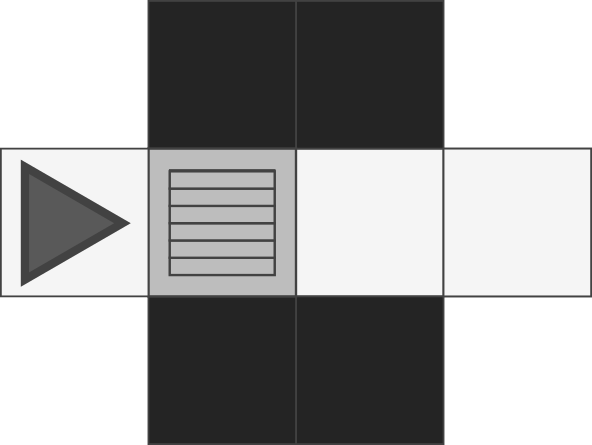
\includegraphics[width=0.4\linewidth]{pictures/TunnelMacro.png}
    \caption[Tunnel Macro]{Tunnel Macro\\ Instead of R, the move RR is generated}
    \label{fig:tunnelmacro}
\end{figure}
\begin{figure}[ht]
    \centering
    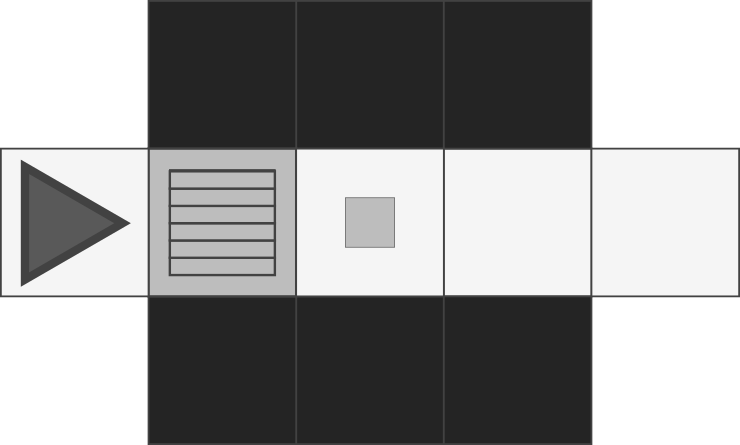
\includegraphics[width=0.5\linewidth]{pictures/TunnelMacroException.png}
    \caption[Tunnel Macro Exception]{Tunnel Macro Exception\\ The move R is generated to push the box on the goal. The next time available moves are computed, move RR will be generated}
    \label{fig:tunnelmacroexception}
\end{figure}

\subsection{Goal Macros}
Goal Macros are used to identify the order with which goals are covered by boxes inside a goal room. A goal room is an area of the board with at least three adjacent boxes, which tries to maximize the number of squares and minimize the number of entrances and the number of boxes, according to the following formula
\begin{equation}
    GRoomScore = 1000*(20-en)+5*sq- 100*man\_io- 500*boxes
\end{equation}
where $en$ is the number of entrances, $sq$ is the number of squares, $man\_io$ are entrances from which the pusher can enter the goal room but he cannot push a box through and $boxes$ is the number of boxes inside the goal room. If a suitable goal room is found, the next step is to build the Goal Macro Tree. The Goal Macro Tree contains for each node a hash that represents the boxes on the goal room's goals, a sequence of pairs entrance-goal that represent the goal that the box should be pushed to if it was on that entrance and a sequence of moves that can be used to execute the macro. During moves generation, if a box is about to be pushed to an entrance square, the tree is accessed to retrieve the move sequence. If the move sequence is valid in the current state, it's substituted to the single push. If the sequence is not valid, an online search is executed by considering a sub-problem in which every other box is turned into a wall and the only valid goal is the one that should be filled by the macro. If the search is successful, the sequence is used as a macro, otherwise the single push is used.

\subsection{Goal Cuts}
Goal Cuts are a simple improvement over Goal Macros for which instead of adding the Goal Macro to the list of available moves in the current states, it is returned as the only move available.
\chapter{Experimental results}
\label{experiments}
In this chapter we compare the performance of IDA* and various versions of MCTS on Samegame and Sokoban.

\section{Samegame}
As a preliminary part of our study, we replicated the experiment performed by Schadd et al. \cite{DBLP:journals/kbs/SchaddWTU12} and compared our results. We ran an experiment using our implementation of SP-MCTS. Due to differences of the Samegame implementation, our program was considerably slower than the one used in \cite{DBLP:journals/kbs/SchaddWTU12}. Our implementation performed an average of 2630 iterations per second against the 13888 iterations per second obtained by \cite{DBLP:journals/kbs/SchaddWTU12}. The program used in \cite{DBLP:journals/kbs/SchaddWTU12} performed 100000 iterations and 1000 restarts with search time distributed per move, which --- considering an average solution length of 64.4 --- resulted in an average of 1553 iterations per move. We decided to keep execution time as a constraint instead of number of iterations, and to achieve that, we reduced the number of randomized restarts from 1000 to 180. The resulting MCTS configuration used a UCT constant of 4.31, a SP-MCTS constant of 96.67, 1500 iterations per move and 180 restarts. As a result, we obtained a score of 73586 in the standard test set \cite{highscore}. Table \ref{tab:samegame_spmctsresults} shows the results for each level in the test set in comparison with the results obtained by \cite{DBLP:journals/kbs/SchaddWTU12} and HGSTS \cite{Edelkamph}, the top scoring documented algorithm for Samegame.
\begin{table}[!h]
    \centering
    \begin{tabular}{ l | l | l | l }
          \# & Our SP-MCTS & SP-MCTS(3) & HGSTS \\
          \hline			
          1 & 2671 & 2919 & 2561 \\
          2 & 3723 & 3797 & 4995 \\
          3 & 3051 & 3243 & 2858 \\
          4 & 3781 & 3687 & 4051 \\
          5 & 4001 & 4067 & 4633 \\
          6 & 4189 & 4269 & 5003 \\
          7 & 2359 & 2949 & 2717 \\
          8 & 3881 & 4043 & 4622 \\
          9 & 4723 & 4769 & 6086 \\
          10 & 2623 & 3245 & 3628 \\
          11 & 2689 & 3259 & 2796 \\
          12 & 3083 & 3245 & 3710 \\
          13 & 2881 & 3211 & 3271 \\
          14 & 2687 & 2937 & 2432 \\
          15 & 3021 & 3343 & 3877 \\
          16 & 4915 & 5117 & 6074 \\
          17 & 4717 & 4959 & 5166 \\
          18 & 5109 & 5151 & 6044 \\
          19 & 4843 & 4803 & 5019 \\
          20 & 4639 & 4999 & 5175 \\
          \hline  
          Total & 73586 & 78012 & 84718 \\
          \hline 
    \end{tabular}
    \caption[Our SP-MCTS results]{Results of our implementation of SP-MCTS}
    \label{tab:samegame_spmctsresults}
\end{table}

\medskip\noindent
Our results are overall worse than the ones obtained by the original authors, but considering the difference in the number of restarts, such outcome is in line with what we expected. This experiment allowed us to ensure that our implementation is coherent to \cite{DBLP:journals/kbs/SchaddWTU12} and to proceed with further experiments with a baseline for performance comparisons.

\subsection{Node Elimination \& Cycles Avoidance}
We started our optimizations analysis with Node Elimination. To reduce computation time we performed the tests with 1500 iterations without randomized restarts. The baseline was obtained with SP-MCTS and no other optimization. We then enabled Node Elimination and compared the results, shown in Table \ref{tab:samegame_nodeelimination}.
\begin{table}[!h]
    \centering
    \begin{tabular}{l|l}
        Configuration & Score\\
        \hline
        Baseline & 57965 \\
        Node Elimination & 56940
    \end{tabular}
    \caption{Node Elimination outcome}
    \label{tab:samegame_nodeelimination}
\end{table}
Node Elimination obtained a score lower than the baseline. We can assume this is due to the fact that in Samegame revisiting terminal nodes can help in the estimation of the action value function.

\medskip\noindent
Since in Samegame cycles can't occur, there was no need to test Cycles Avoidance.

\subsection{Parameters tuning}
In order to take full advantage of the optimizations we described in Section \ref{proposedsolution}, we needed to tune their parameters to obtain the best configuration. In particular, we executed repeated searches with different values for the RAVE threshold and the memory budget of Node Recycling. We also tuned again the UCT constant with UCB1-Tuned, since \cite{DBLP:journals/kbs/SchaddWTU12} performed the tuning with the SP-MCTS formula. Node Elimination has no parameters so it didn't require tuning. As before we performed the tests with 1500 iteration and no randomized restarts. The results of the tuning process are shown in Tables \ref{tab:samegame_tuningrave} and \ref{tab:tuningrecycling}.
\begin{table}[!h]
    \centering
    \begin{tabular}{l|l}
        V & Score \\
        \hline 
        1 & 57965 \\
        5 & 46663 \\
        10 & 47722 \\
        15 & 49519 \\
        25 & 49239 \\
        50 & 52028 \\
        100 & 54738 \\
    \end{tabular}
    \caption[RAVE thresholds scores]{Scores obtained with different RAVE thresholds. The first row is equivalent to disabling RAVE and represents our baseline.}
    \label{tab:samegame_tuningrave}
\end{table}

\medskip\noindent
 If we only consider the results with RAVE enabled, it reached the highest score with $V=100$, but contrary to our expectations, it had an overall negative impact on the score. We concluded that the assumption upon which RAVE is based, does not hold for Samegame, i.e. moves performed later on in a simulation can't be considered as if they were performed at the beginning.

\begin{table}[!h]
    \centering
    \begin{tabular}{l|l}
        Nodes & Score \\
        \hline 
        300 & 55302 \\
        600 & 57798 \\
        900 & 54601 \\
        1200 & 56532 \\
        1500 & 57965 \\
    \end{tabular}
    \caption[Node Recycling memory budgets scores]{Scores obtained with Node Recycling and different memory budgets. The last row is equivalent to disabling Node Recycling and represents our baseline.}
    \label{tab:tuningrecycling}
\end{table}

\medskip\noindent
Node Recycling reduced the score too, although less than RAVE, which means that it may prune good sub-trees in Samegame. With a memory budget of $600$ nodes it produced a score close to the baseline.

%figures \ref{fig:samegametuning} and \ref{fig:samegameucb1tuning}. 

%\begin{figure}[!h]
%\centering
%\subfigure[Scores obtained with different RAVE thresholds]{
%\label{fig:samegame_tuningrave}
%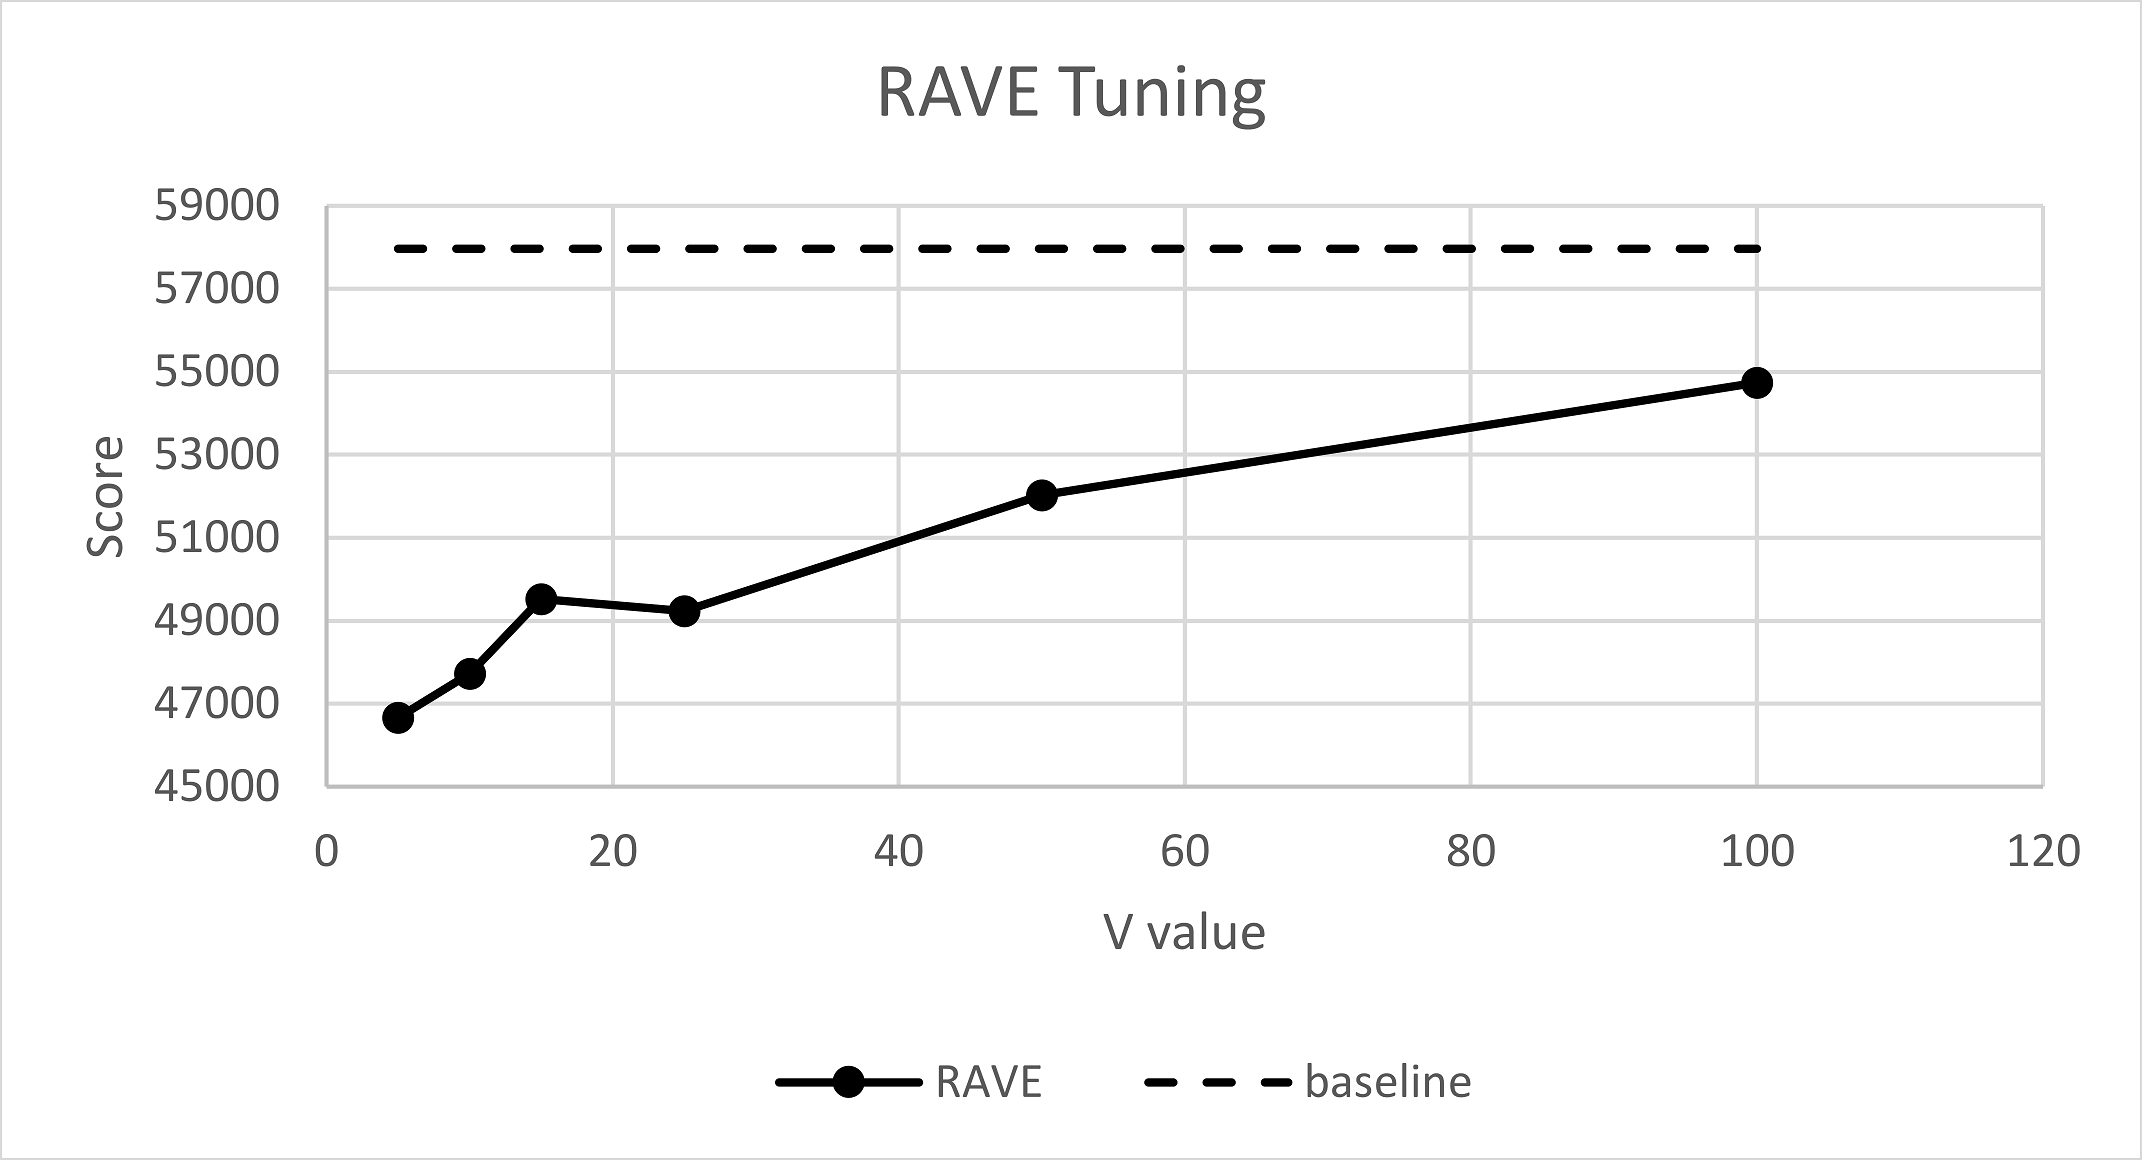
\includegraphics[width=0.8\linewidth]{pictures/SamegameRaveTuning.png}}
%\subfigure[Scores obtained with different memory budgets]{
%\label{fig:samegame_tuningrecycling}
%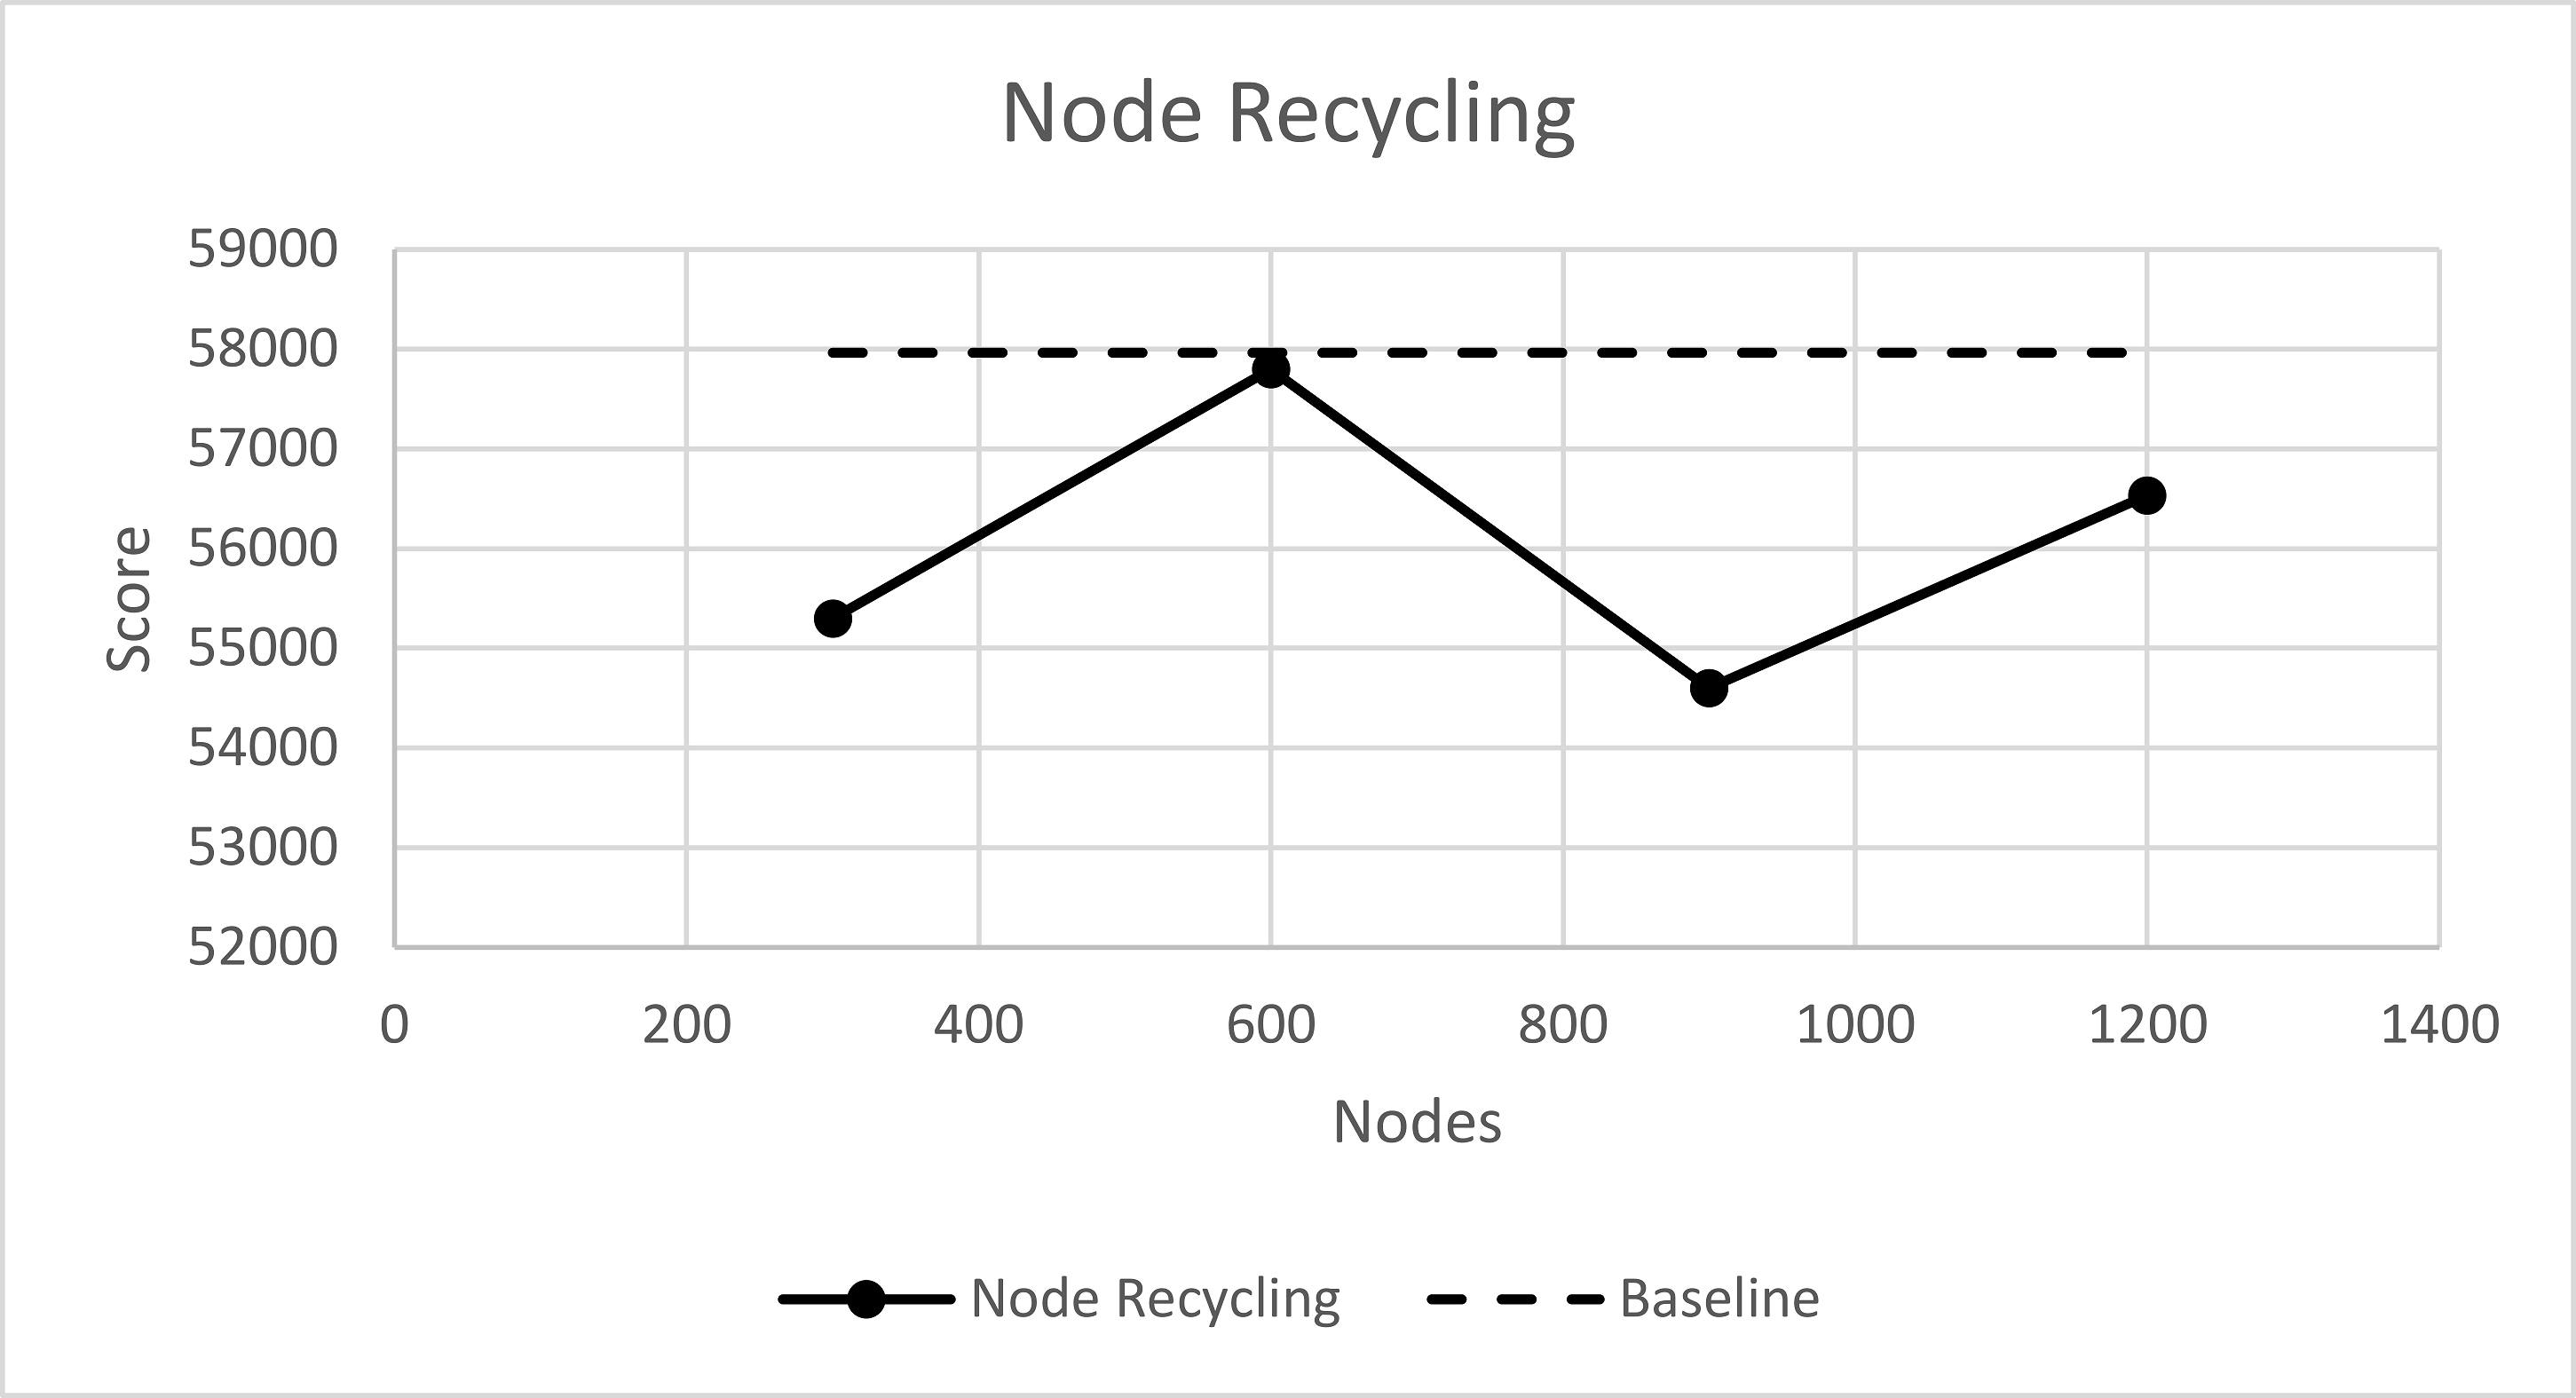
\includegraphics[width=0.8\linewidth]{pictures/SamegameNodeRecyclingTuning.png}}
%\caption{Samegame Tuning}
%\label{fig:samegametuning}
%\end{figure}

\medskip\noindent
As shown in Figure \ref{fig:samegameucb1tuning}, UCB1-Tuned performed better than SP-MCTS with different values but reached the highest score with a constant value of 10.

\begin{figure}[!h]
    \centering
    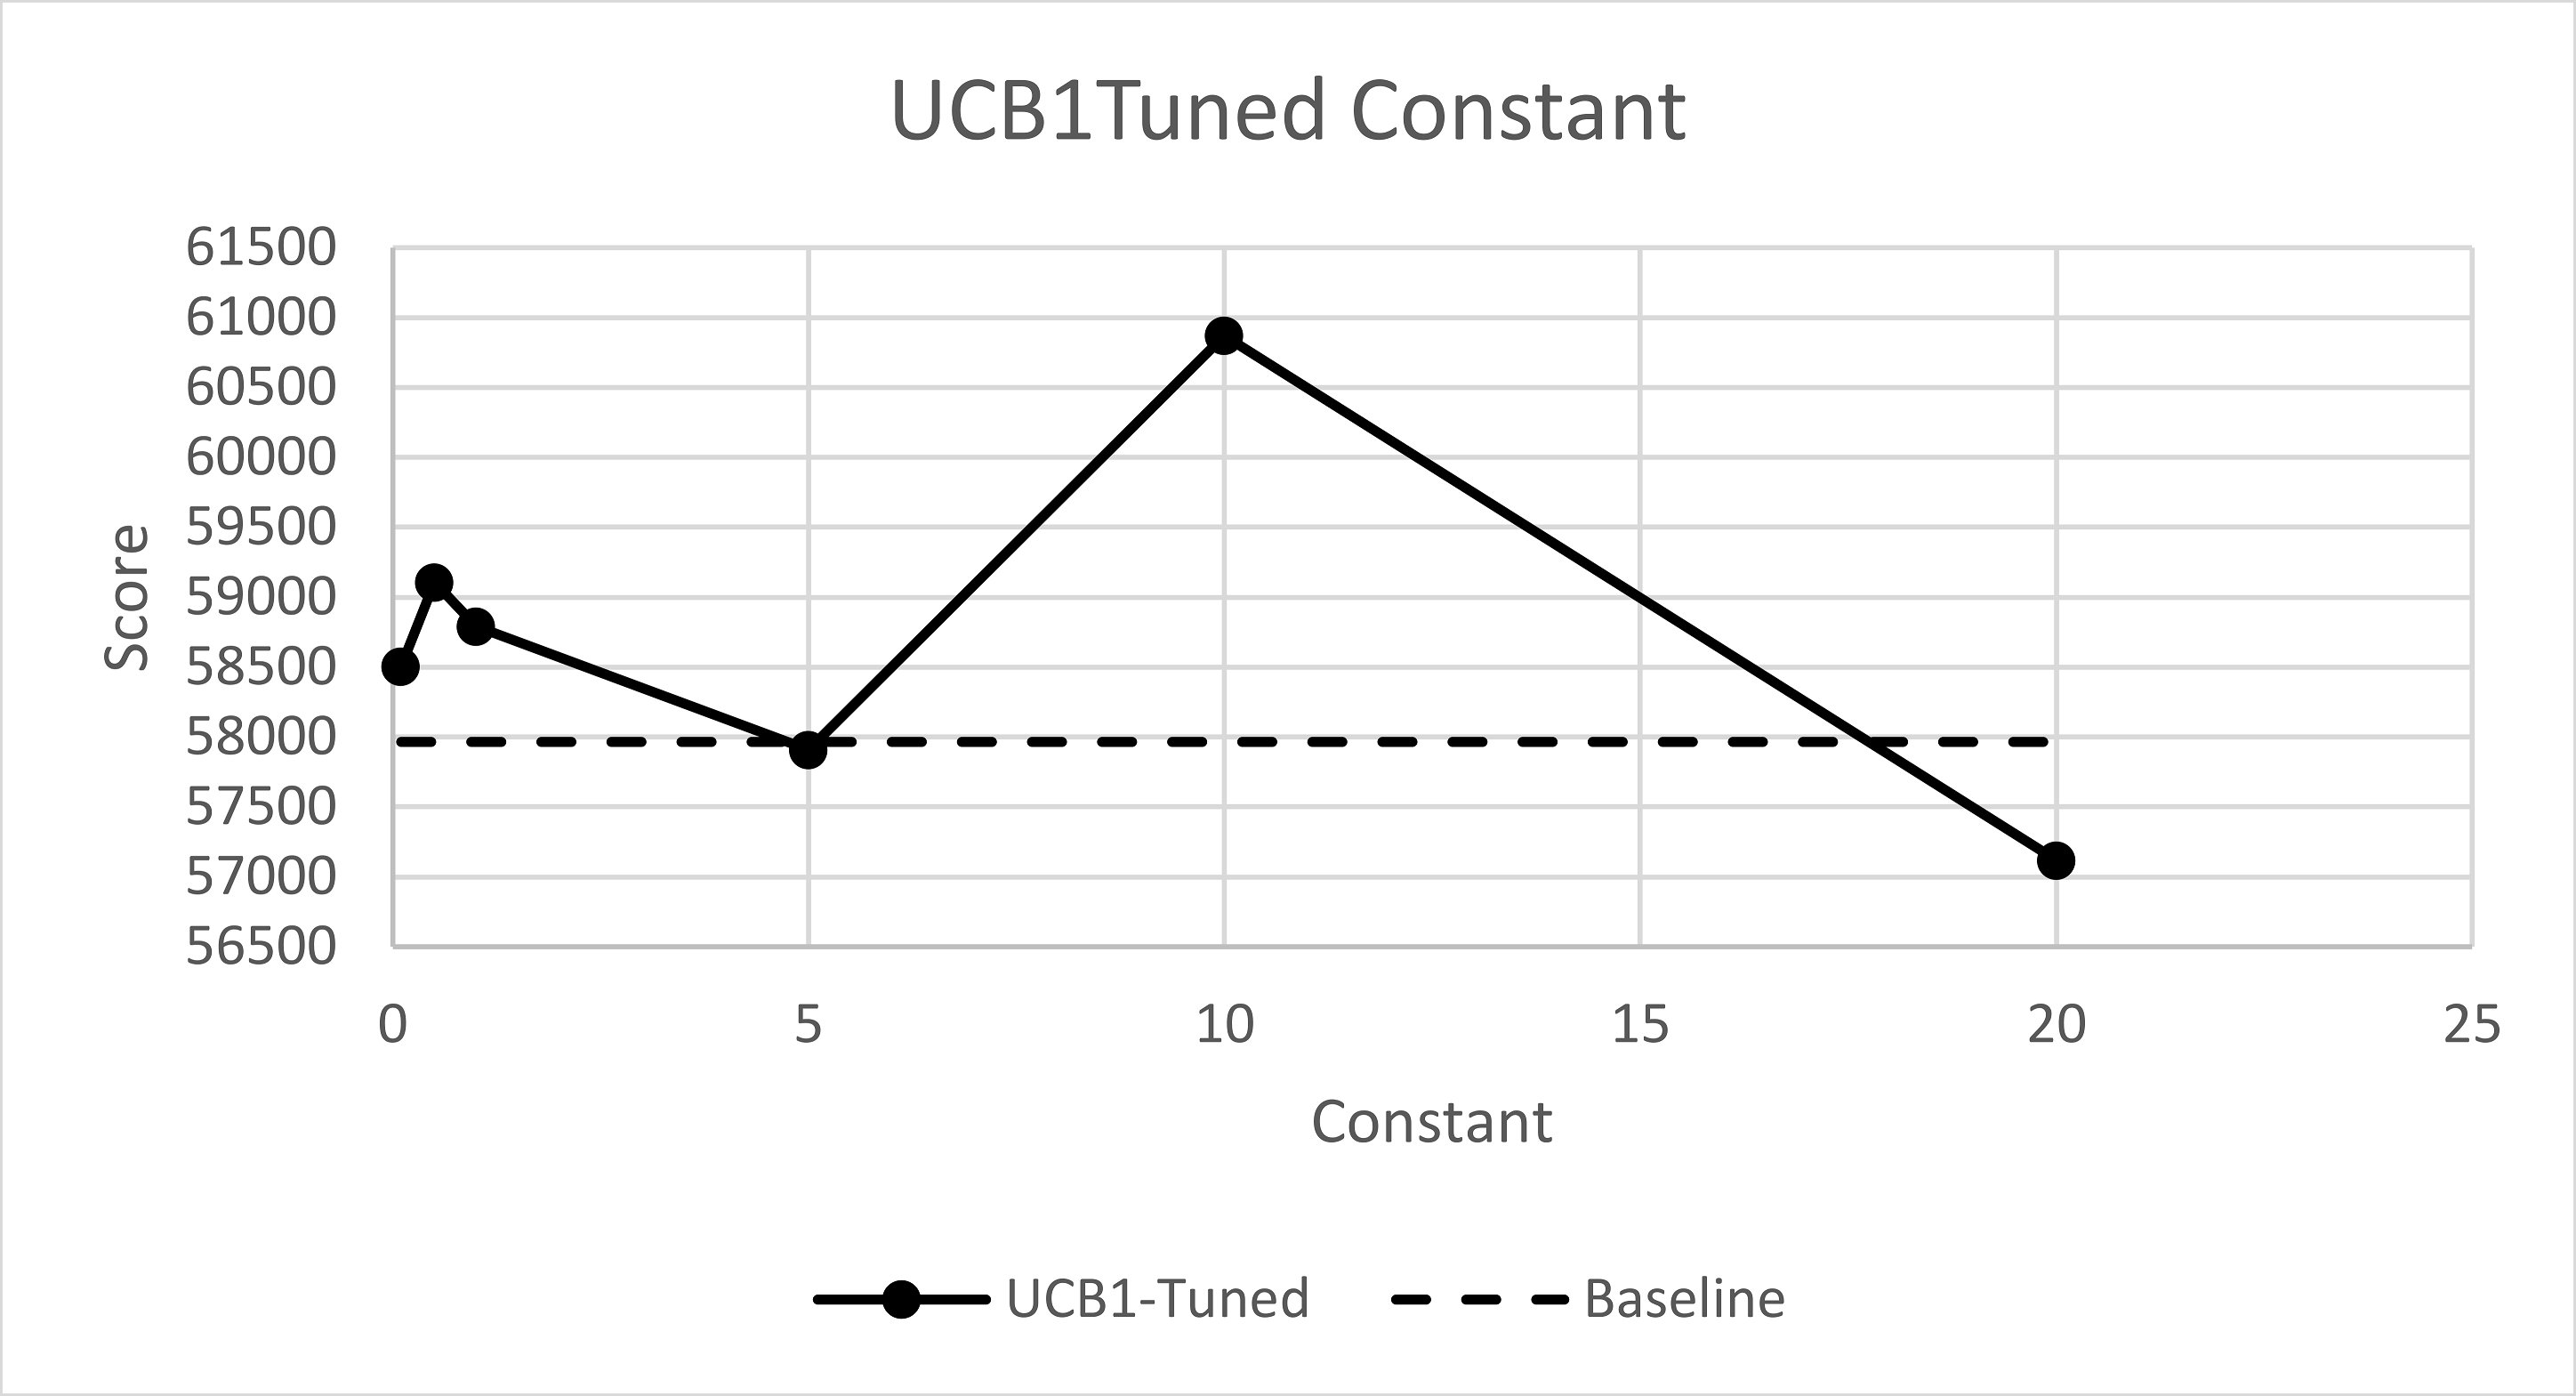
\includegraphics[width=0.8\linewidth]{pictures/SamegameUCB1Tuned.png}
    \caption[UCB1-Tuned constants scores]{Scores obtained with different constant values}
    \label{fig:samegameucb1tuning}
\end{figure}

\subsection{Results}
Considering the results obtained in previous experiments, we performed a comparison between our basic version of SP-MCTS and SP-MCTS with UCB1-Tuned. For this evaluation we used 1500 iterations and 180 restarts. The results of this comparison can be seen in Table \ref{tab:samegame_optresults}. UCB1-Tuned obtained a score of 74136, surpassing our previous score by 550 points.

\begin{table}[!h]
    \centering
    \begin{tabular}{ l | l | l }
          \# & Our SP-MCTS & UCB1-Tuned \\
          \hline			
          1 & 2671 & 2615 \\
          2 & 3723 & 3763\\
          3 & 3051 & 3251\\
          4 & 3781 & 3607\\
          5 & 4001 & 3891\\
          6 & 4189 & 4147\\
          7 & 2359 & 2675\\
          8 & 3881 & 3875\\
          9 & 4723 & 4689\\
          10 & 2623 & 2601\\
          11 & 2689 & 2683\\
          12 & 3083 & 3125\\
          13 & 2881 & 2805\\
          14 & 2687 & 2687\\
          15 & 3021 & 3329\\
          16 & 4915 & 4891\\
          17 & 4717 & 4639\\
          18 & 5109 & 5117\\
          19 & 4843 & 4869\\
          20 & 4639 & 4877\\
          \hline  
          Total & 73586 & 74136\\
          \hline 
    \end{tabular}
    \caption[SP-MCTS versus UCB1-Tuned in Samegame]{Comparison between results obtained by our SP-MCTS implementation and UCB1-Tuned enhancement.}
    \label{tab:samegame_optresults}
\end{table}

\medskip\noindent
Finally we performed an experiment to compare our optimized SP-MCTS against our version of the IDA* algorithm. \cite{DBLP:journals/kbs/SchaddWTU12} proposed an upper bound on the score for Samegame by considering all blocks of the same color as adjacent. The bonus of $1000$ points for clearing the board is also awarded unless there exists a color of which a single block is remaining. We ran an experiment with IDA* using the same heuristic and a maximum of 7500000 nodes, giving approximately two hours of search time for each level. The results of this experiment can be seen in Table \ref{tab:samegame_mcts_vs_ida*} compared with the best results obtained by MCTS. MCTS strongly outperformed IDA*, which with 9882 points performed at the level of a human beginner.

\begin{table}[!h]
    \centering
    \begin{tabular}{ l | l | l }
          \# & Optimized MCTS & IDA* \\
          \hline			
          1 & 2615 & 415 \\
          2 & 3763 & 387 \\
          3 & 3251 & 378 \\
          4 & 3607 & 670 \\
          5 & 3891 & 592 \\
          6 & 4147 & 655 \\
          7 & 2675 & 435 \\
          8 & 3875 & 505 \\
          9 & 4689 & 518 \\
          10 & 2601 & 572 \\
          11 & 2683 & 295 \\
          12 & 3125 & 543 \\
          13 & 2805 & 643 \\
          14 & 2687 & 177 \\
          15 & 3329 & 545 \\
          16 & 4891 & 321 \\
          17 & 4639 & 457 \\
          18 & 5117 & 573 \\
          19 & 4869 & 541 \\
          20 & 4877 & 660 \\
          \hline  
          Total & 73586 & 9882 \\
          \hline 
    \end{tabular}
    \caption[Optimized MCTS versus IDA* in Samegame]{Results obtained by comparing Optimized MCTS algorithm with IDA*}
    \label{tab:samegame_mcts_vs_ida*}
\end{table}
\section{Sokoban}
Contrary to Samegame, where the reward function was defined as a part of the game rules, in Sokoban we had to define a reward function. In order to determine which among those defined in Section\ref{rewardtype} performed better, we compared them using different UCT constant values. We used the 155 levels of the Microban \cite{microban} suite as a test set throughout all experiments.

\subsection{Reward types}
All tests were performed with random rollouts, Avoid Cycles and Node Elimination enabled. Furthermore, the search was stopped as soon as a solution was found. Figures \ref{fig:constant_InverseBM} through \ref{fig:constant_Boxes} show the impact of the constant on the depth of the generated tree and on the portion of solved levels for InverseBM, NegativeBM, R0 and Boxes respectively.

\medskip\noindent
The optimal value for rewards has been proven to be $C = 1$ for rewards in the range $[0,1]$ \cite{Kocsis:2006:BBM:2091602.2091633}.
Despite having a range between 0 and 1, the best scores for InverseBM were obtained with constants in the range $0.001-0.05$. The tree depth graph shows that with values higher than 0.35 the average depth among all levels remains almost constant. This can be interpreted as the algorithm leaning towards exploration for those values. This unusual behavior may be due to the distribution of the reward function values: while in constant-sum games in the range $[0,1]$ the reward distribution is typically centered on $\frac{1}{2}$ with $0$ and $1$ having the same probability distribution, the InverseBM reward distribution varies according to the level and generally leans towards $0$. This can cause the $0.35$ constant value to assign an higher weight to the exploration part of the UCT formula.
\clearpage

\begin{figure}[!h]
\centering
\subfigure[Trend of generated tree depth using different constant values for reward InverseBM]{
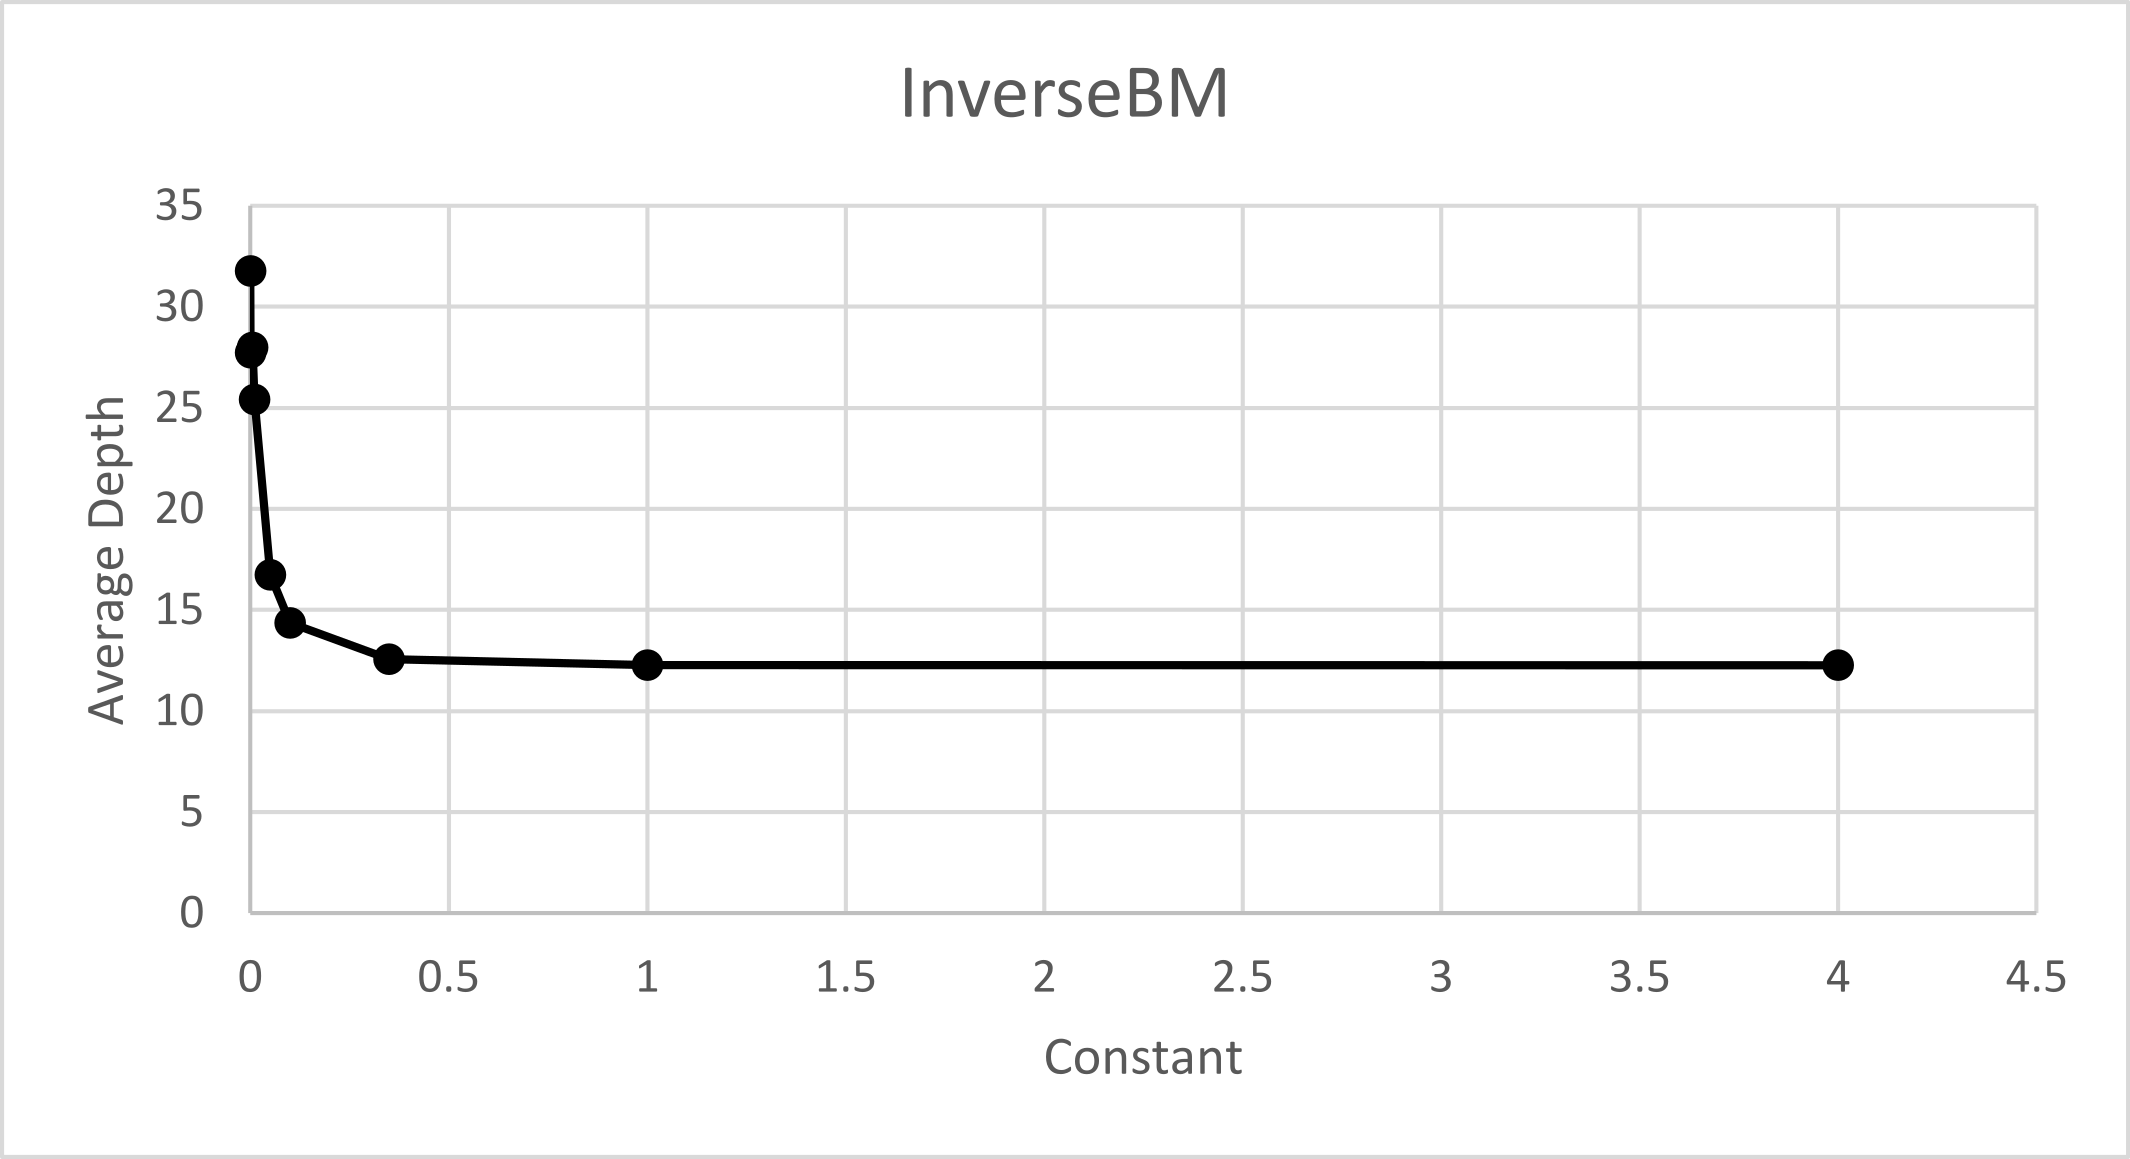
\includegraphics[width=0.8\linewidth]{pictures/InverseDepth.png}}
\subfigure[Trend of solved levels rate using different constant values for reward InverseBM]{
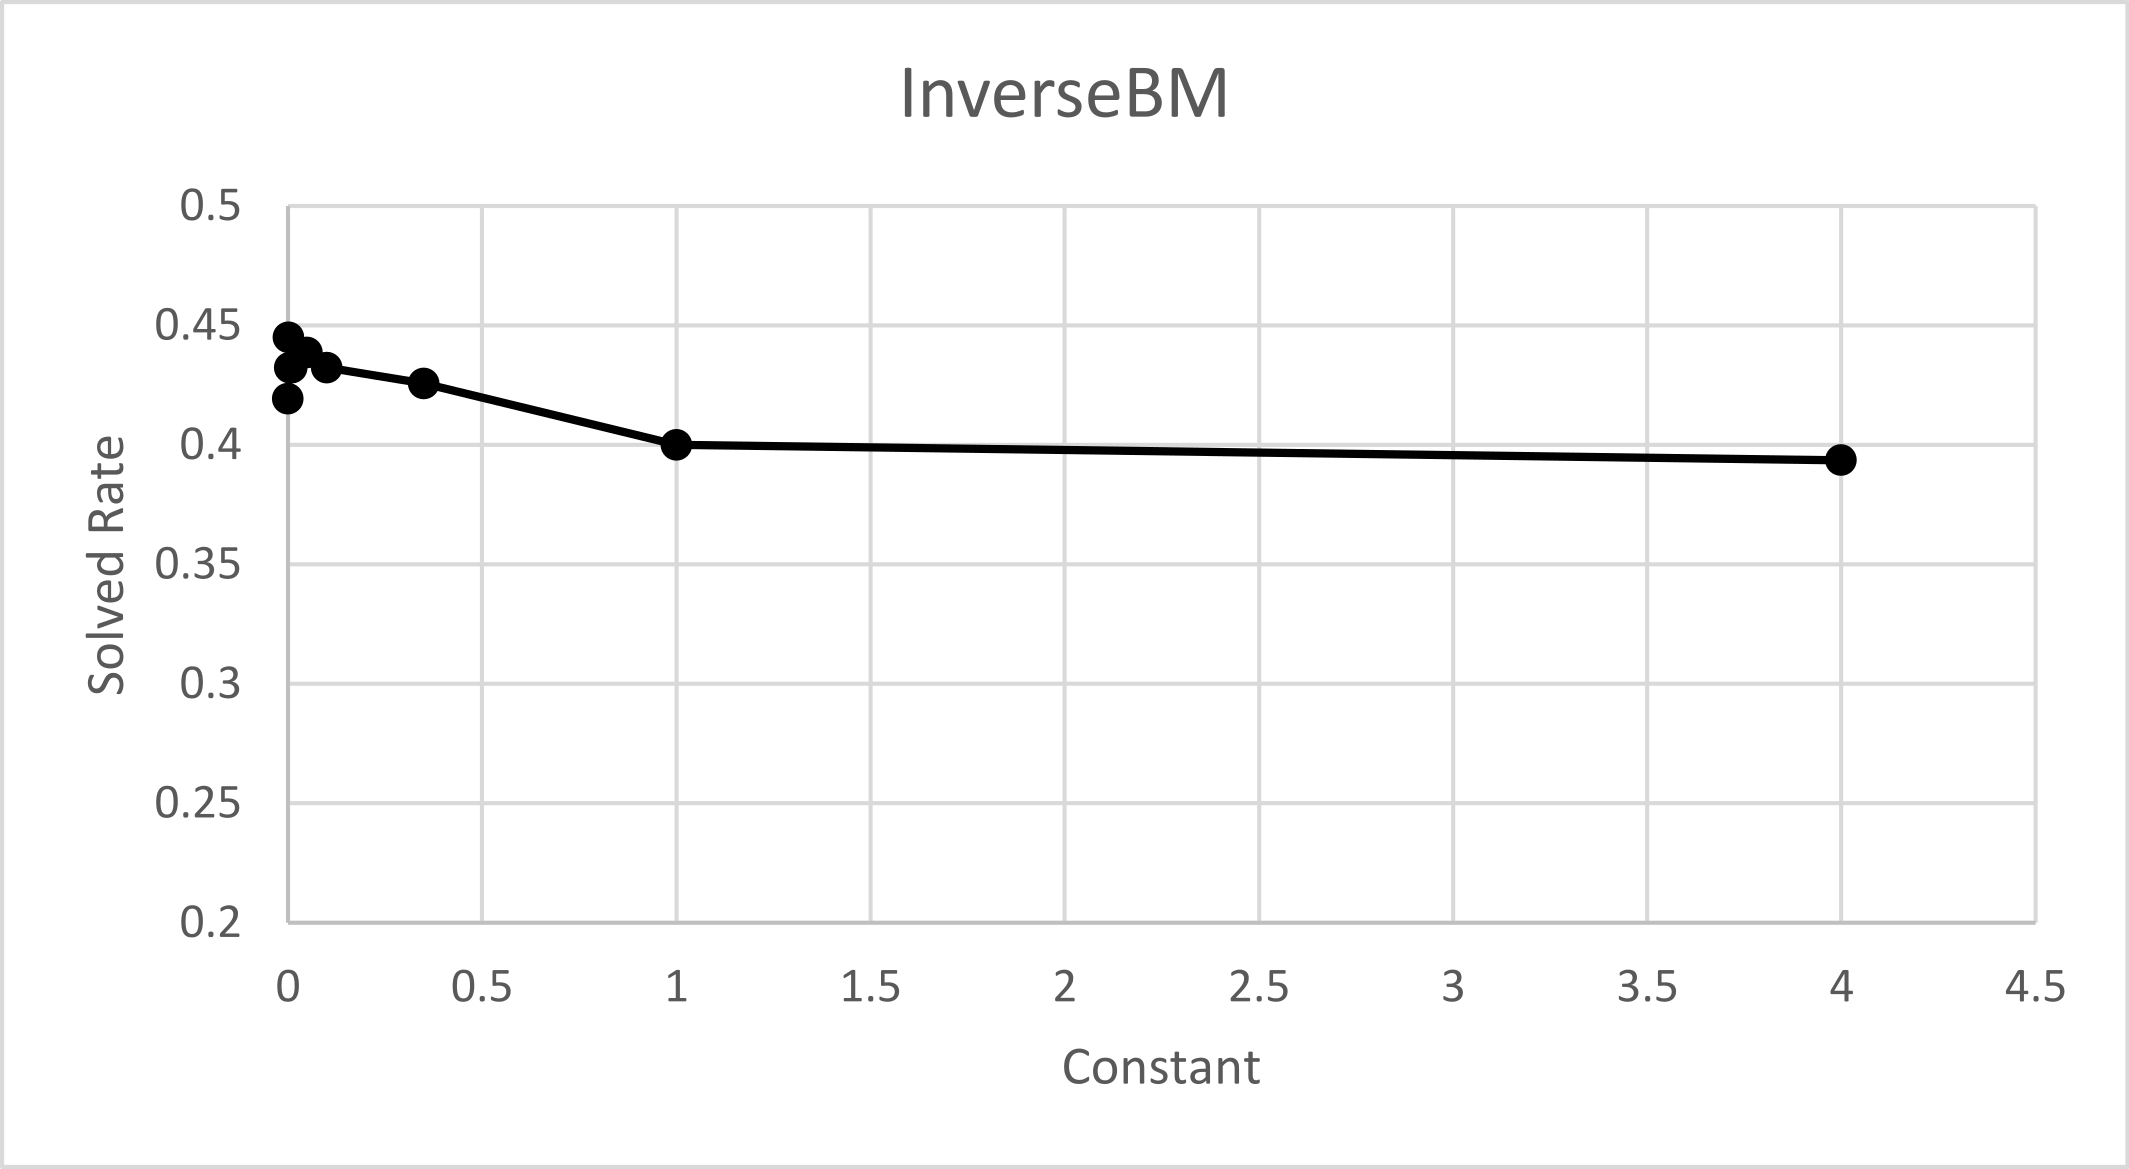
\includegraphics[width=0.8\linewidth]{pictures/InverseSolved.png}}
\caption[InverseBM solved levels rate and tree depth]{}
\label{fig:constant_InverseBM}
\end{figure}
\clearpage

\begin{figure}[!h]
\centering
\subfigure[Trend of generated tree depth using different constant values for reward NegativeBM]{
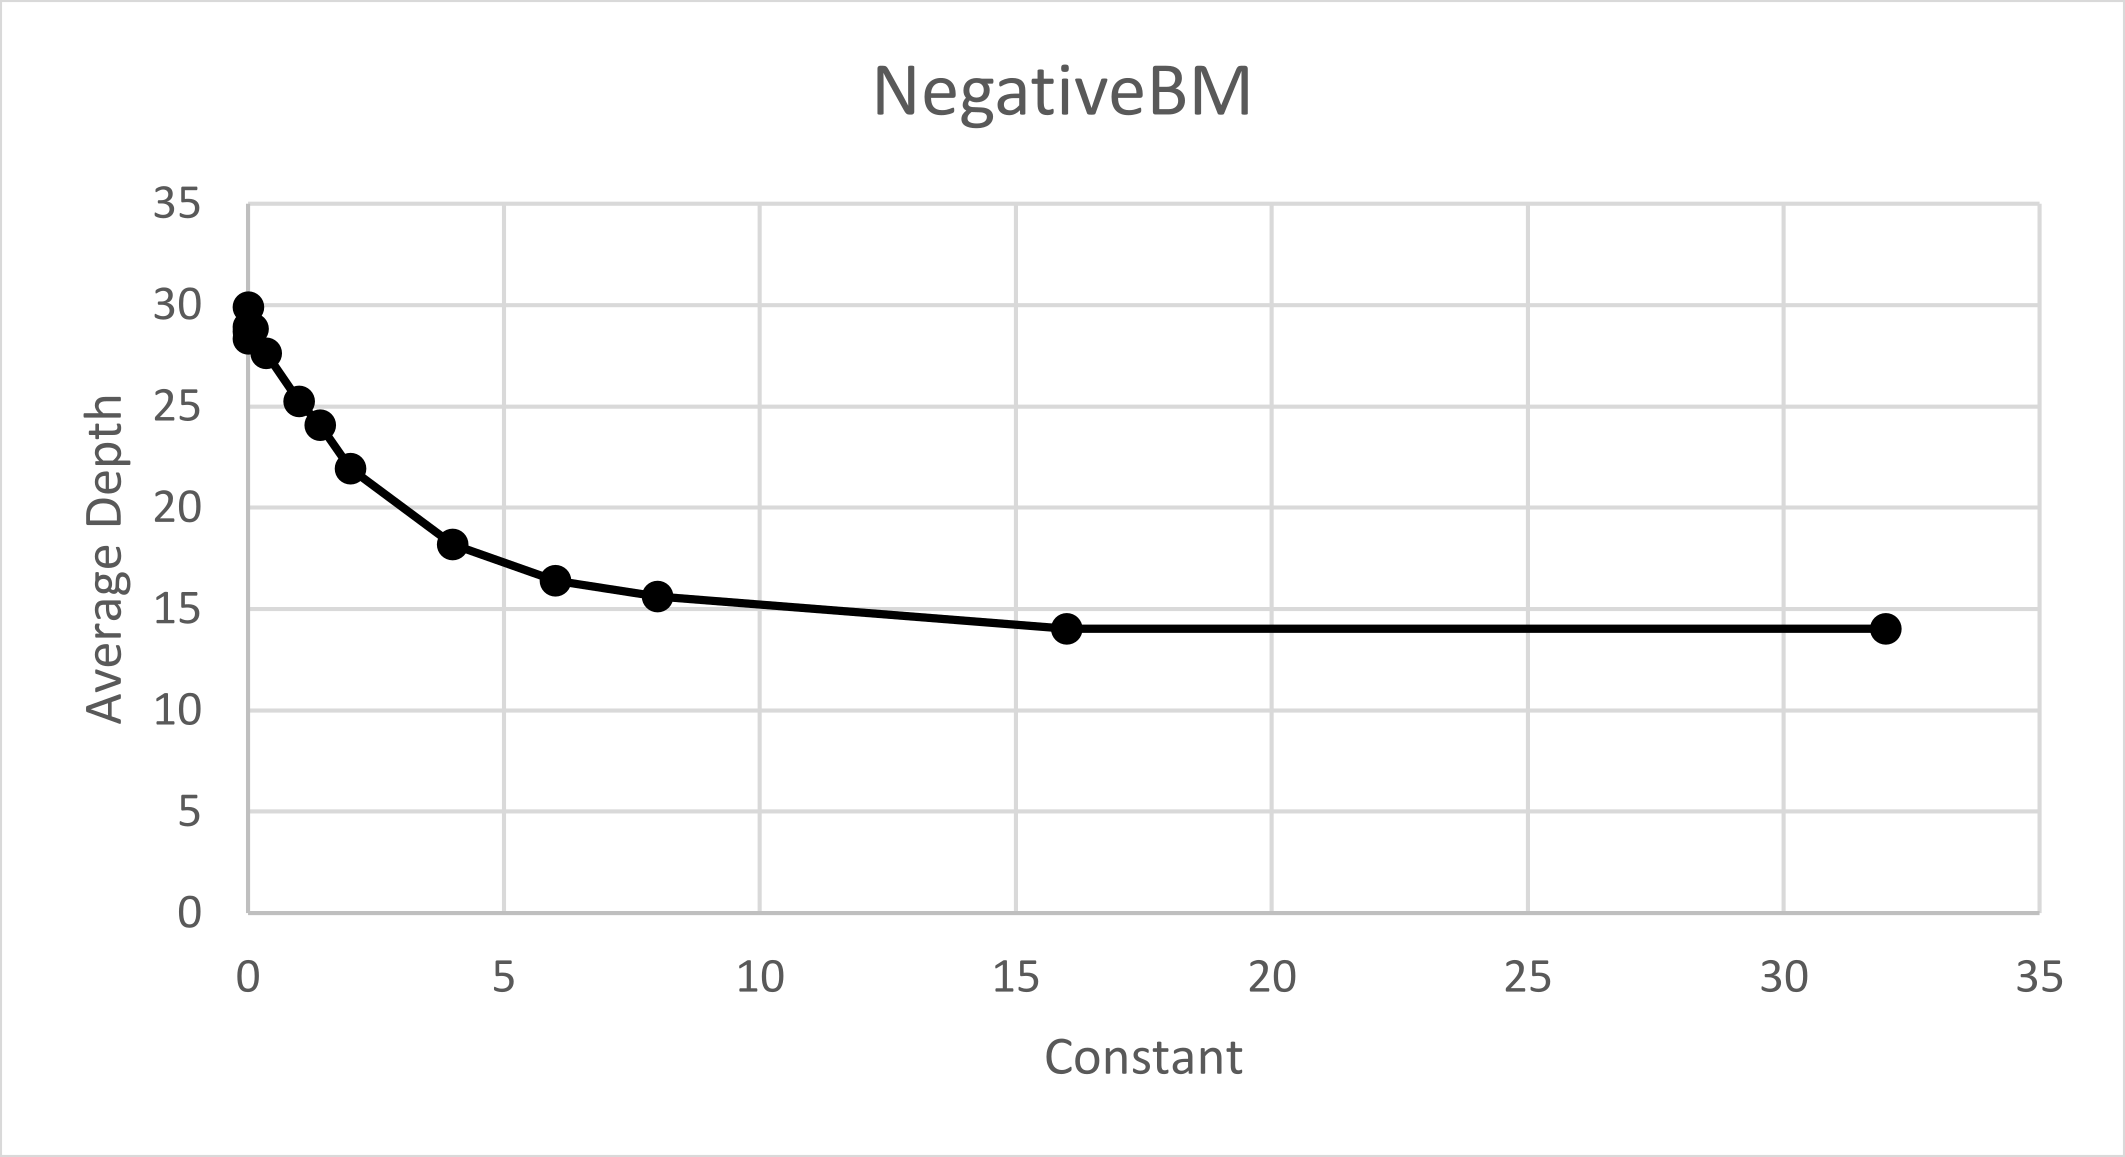
\includegraphics[width=0.8\linewidth]{pictures/NegativeDepth.png}}
\subfigure[Trend of solved levels rate using different constant values for reward NegativeBM]{
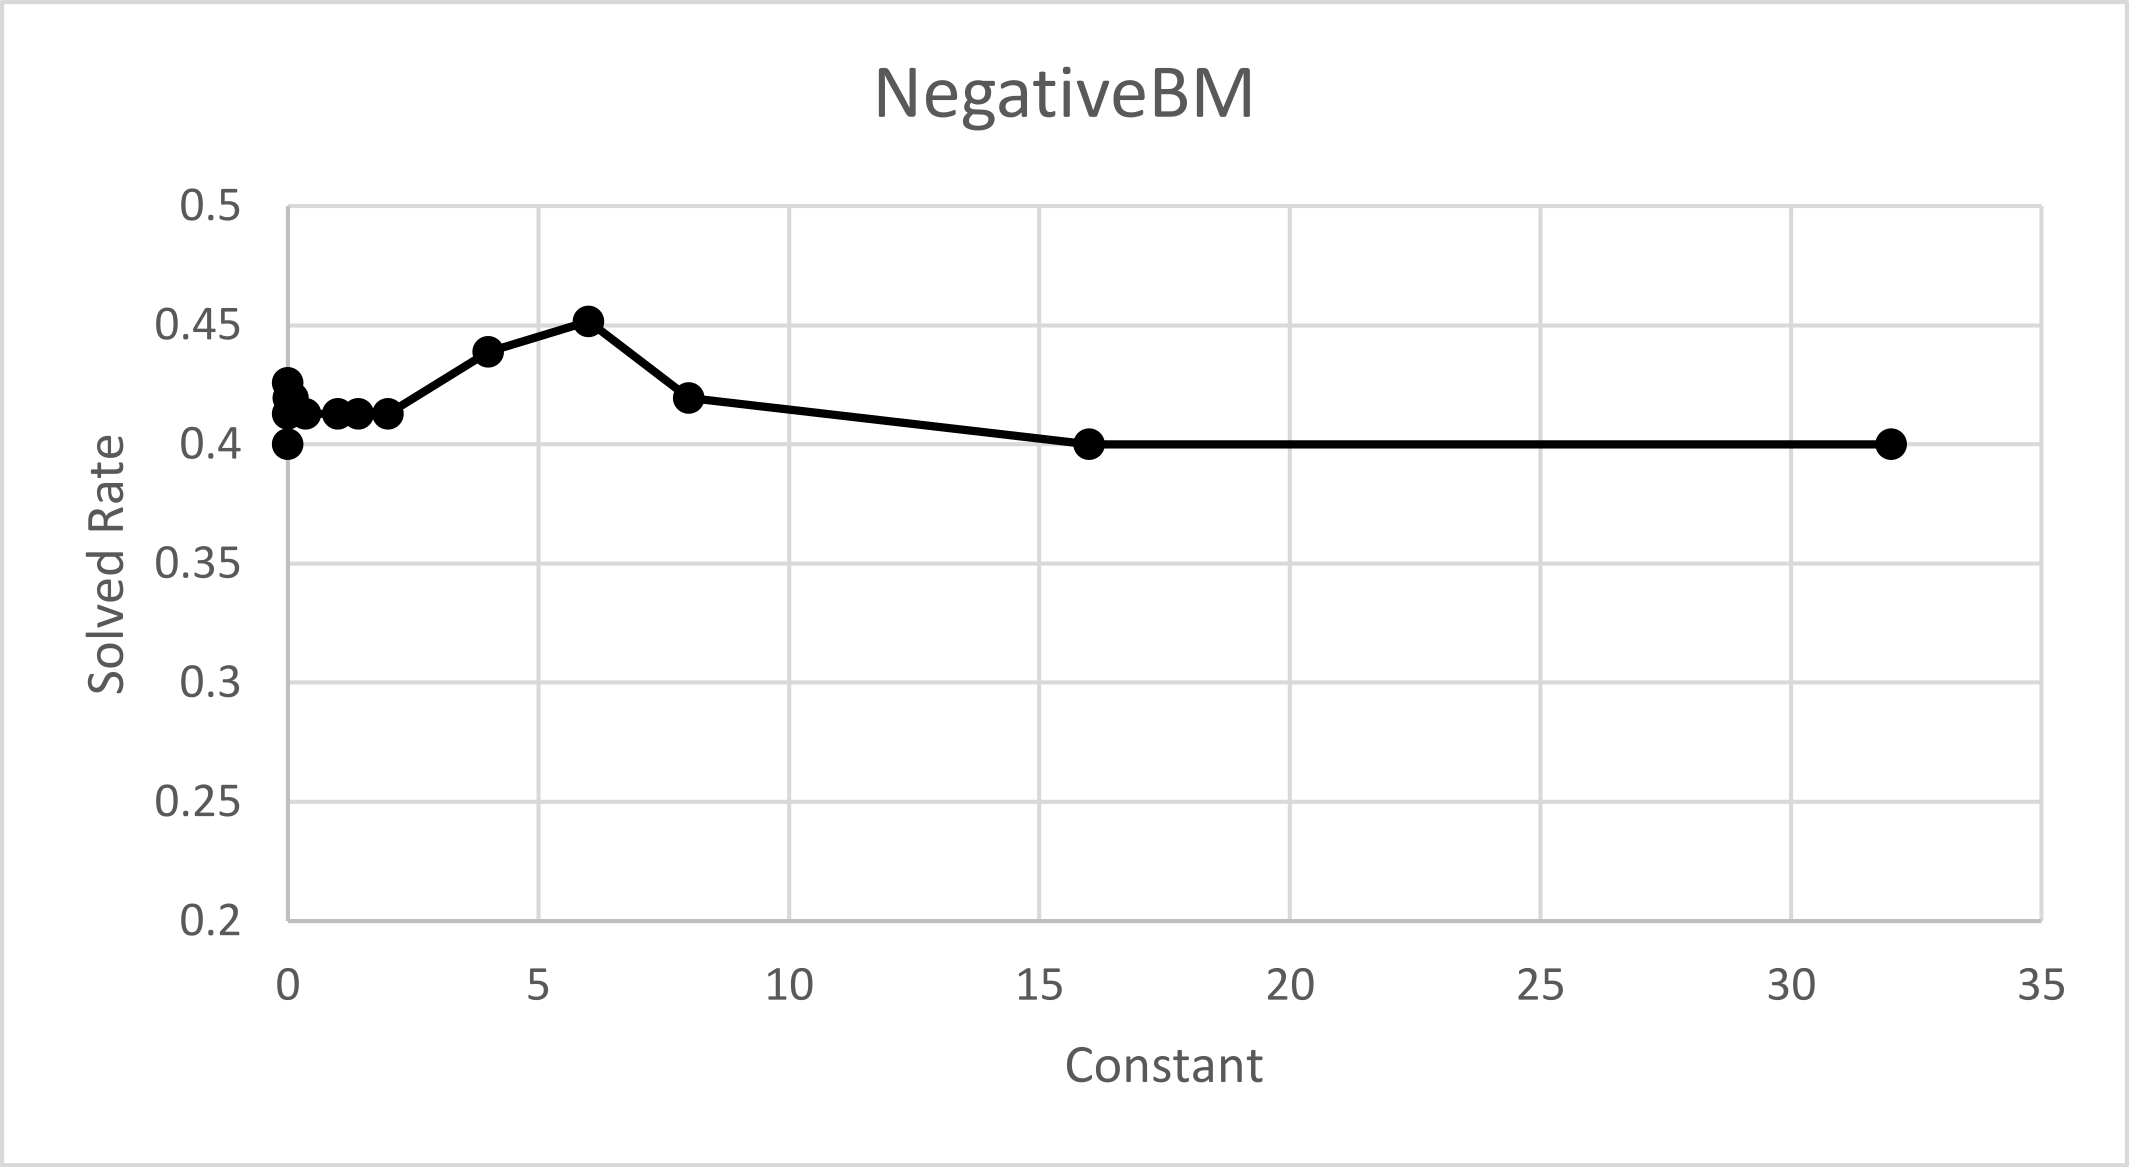
\includegraphics[width=0.8\linewidth]{pictures/NegativeSolved.png}}
\caption[NegativeBM solved levels rate and tree depth]{}
\label{fig:constant_NegativeBM}
\end{figure}

\medskip\noindent
NegativeBM reaches its maximum score with a constant value of 6 and the generated tree depth decreases more gradually due to the larger reward range.
\clearpage

\begin{figure}[!h]
\centering
\subfigure[Trend of generated tree depth using different constant values for reward R0]{
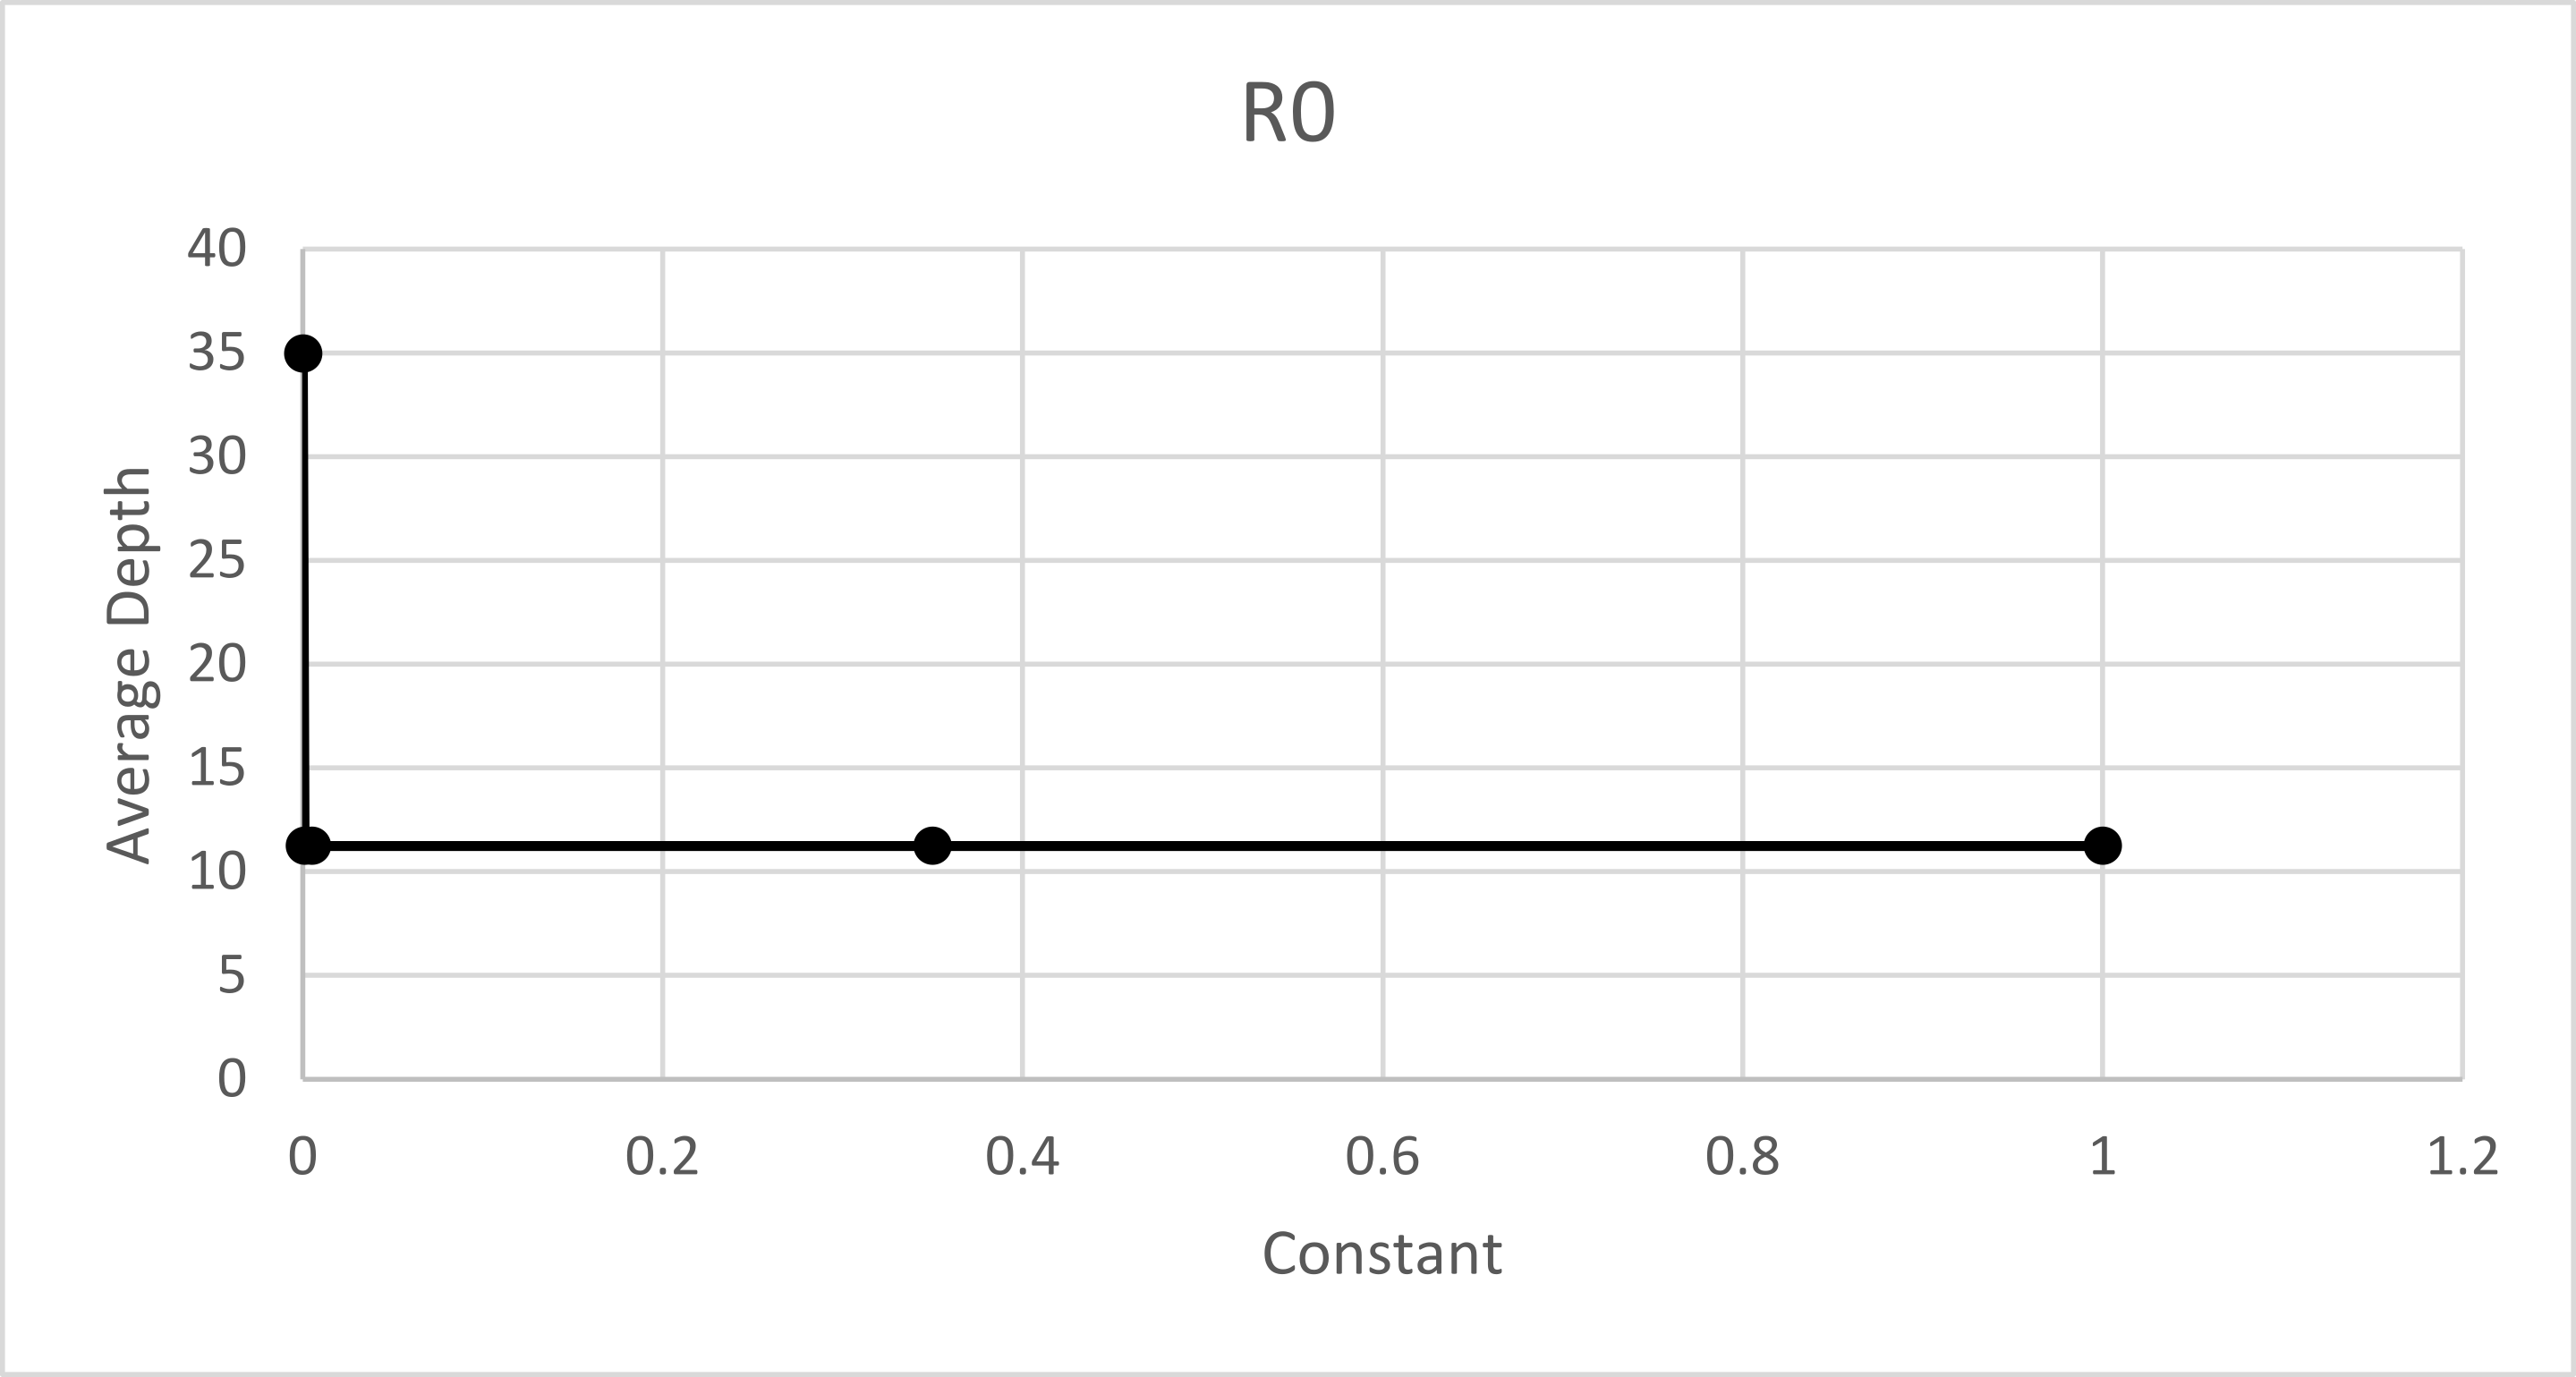
\includegraphics[width=0.8\linewidth]{pictures/R0Depth.png}}
\subfigure[Trend of solved levels rate using different constant values for reward R0]{
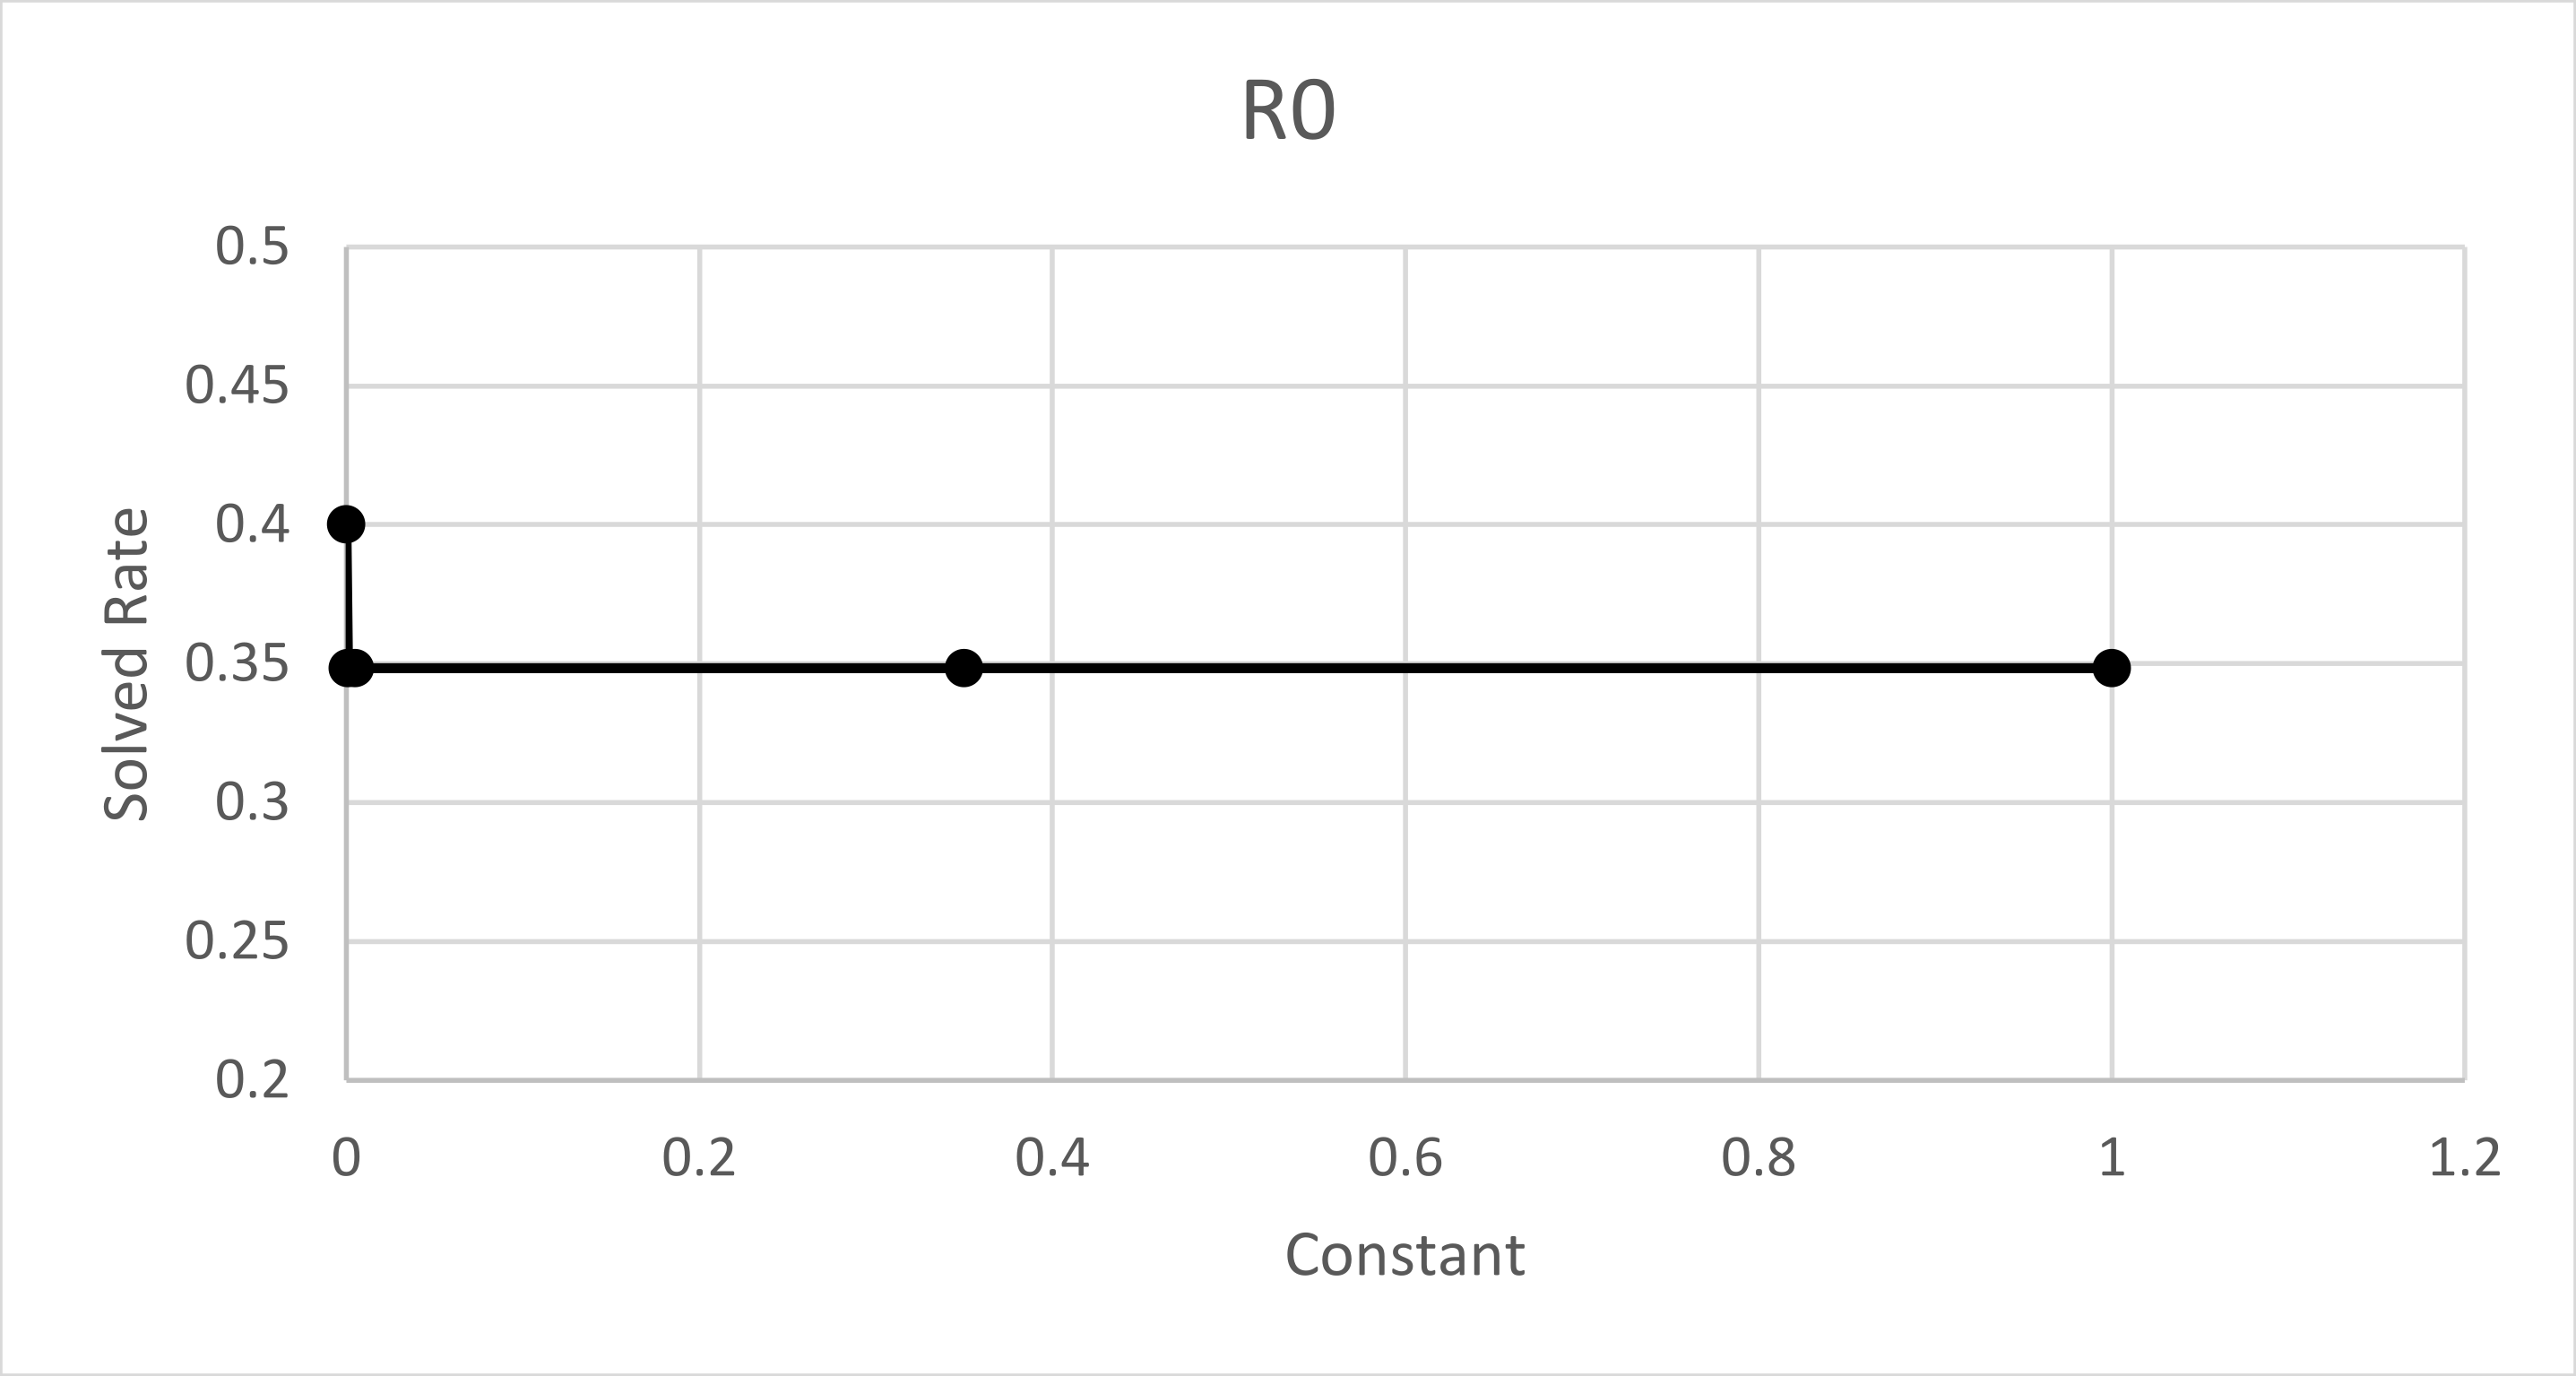
\includegraphics[width=0.8\linewidth]{pictures/R0Solved.png}}
\caption[R0 solved levels rate and tree depth]{}
\label{fig:constant_R0}
\end{figure}

\medskip\noindent
R0 charts clearly show how this reward type is not suitable for solving Sokoban using MCTS. The depth of the trees confirms what we suspected: with the reward being 0 for every rollout except for the last one (since the search is stopped at the first solution), the only relevant part of the UCT formula is the exploration component, which means that for every value of the constant greater than 0, the algorithm will perform a pure exploration. In our implementation if two or more nodes have the same UCT value, the selection phase is deterministic and always chooses the node that was generated first. This implies that with the constant equal to 0, all nodes have a UCT value of 0 and the algorithm will perform a pure exploitation.

\begin{figure}[!h]
\centering
\subfigure[Trend of generated tree depth using different constant values for reward Boxes]{
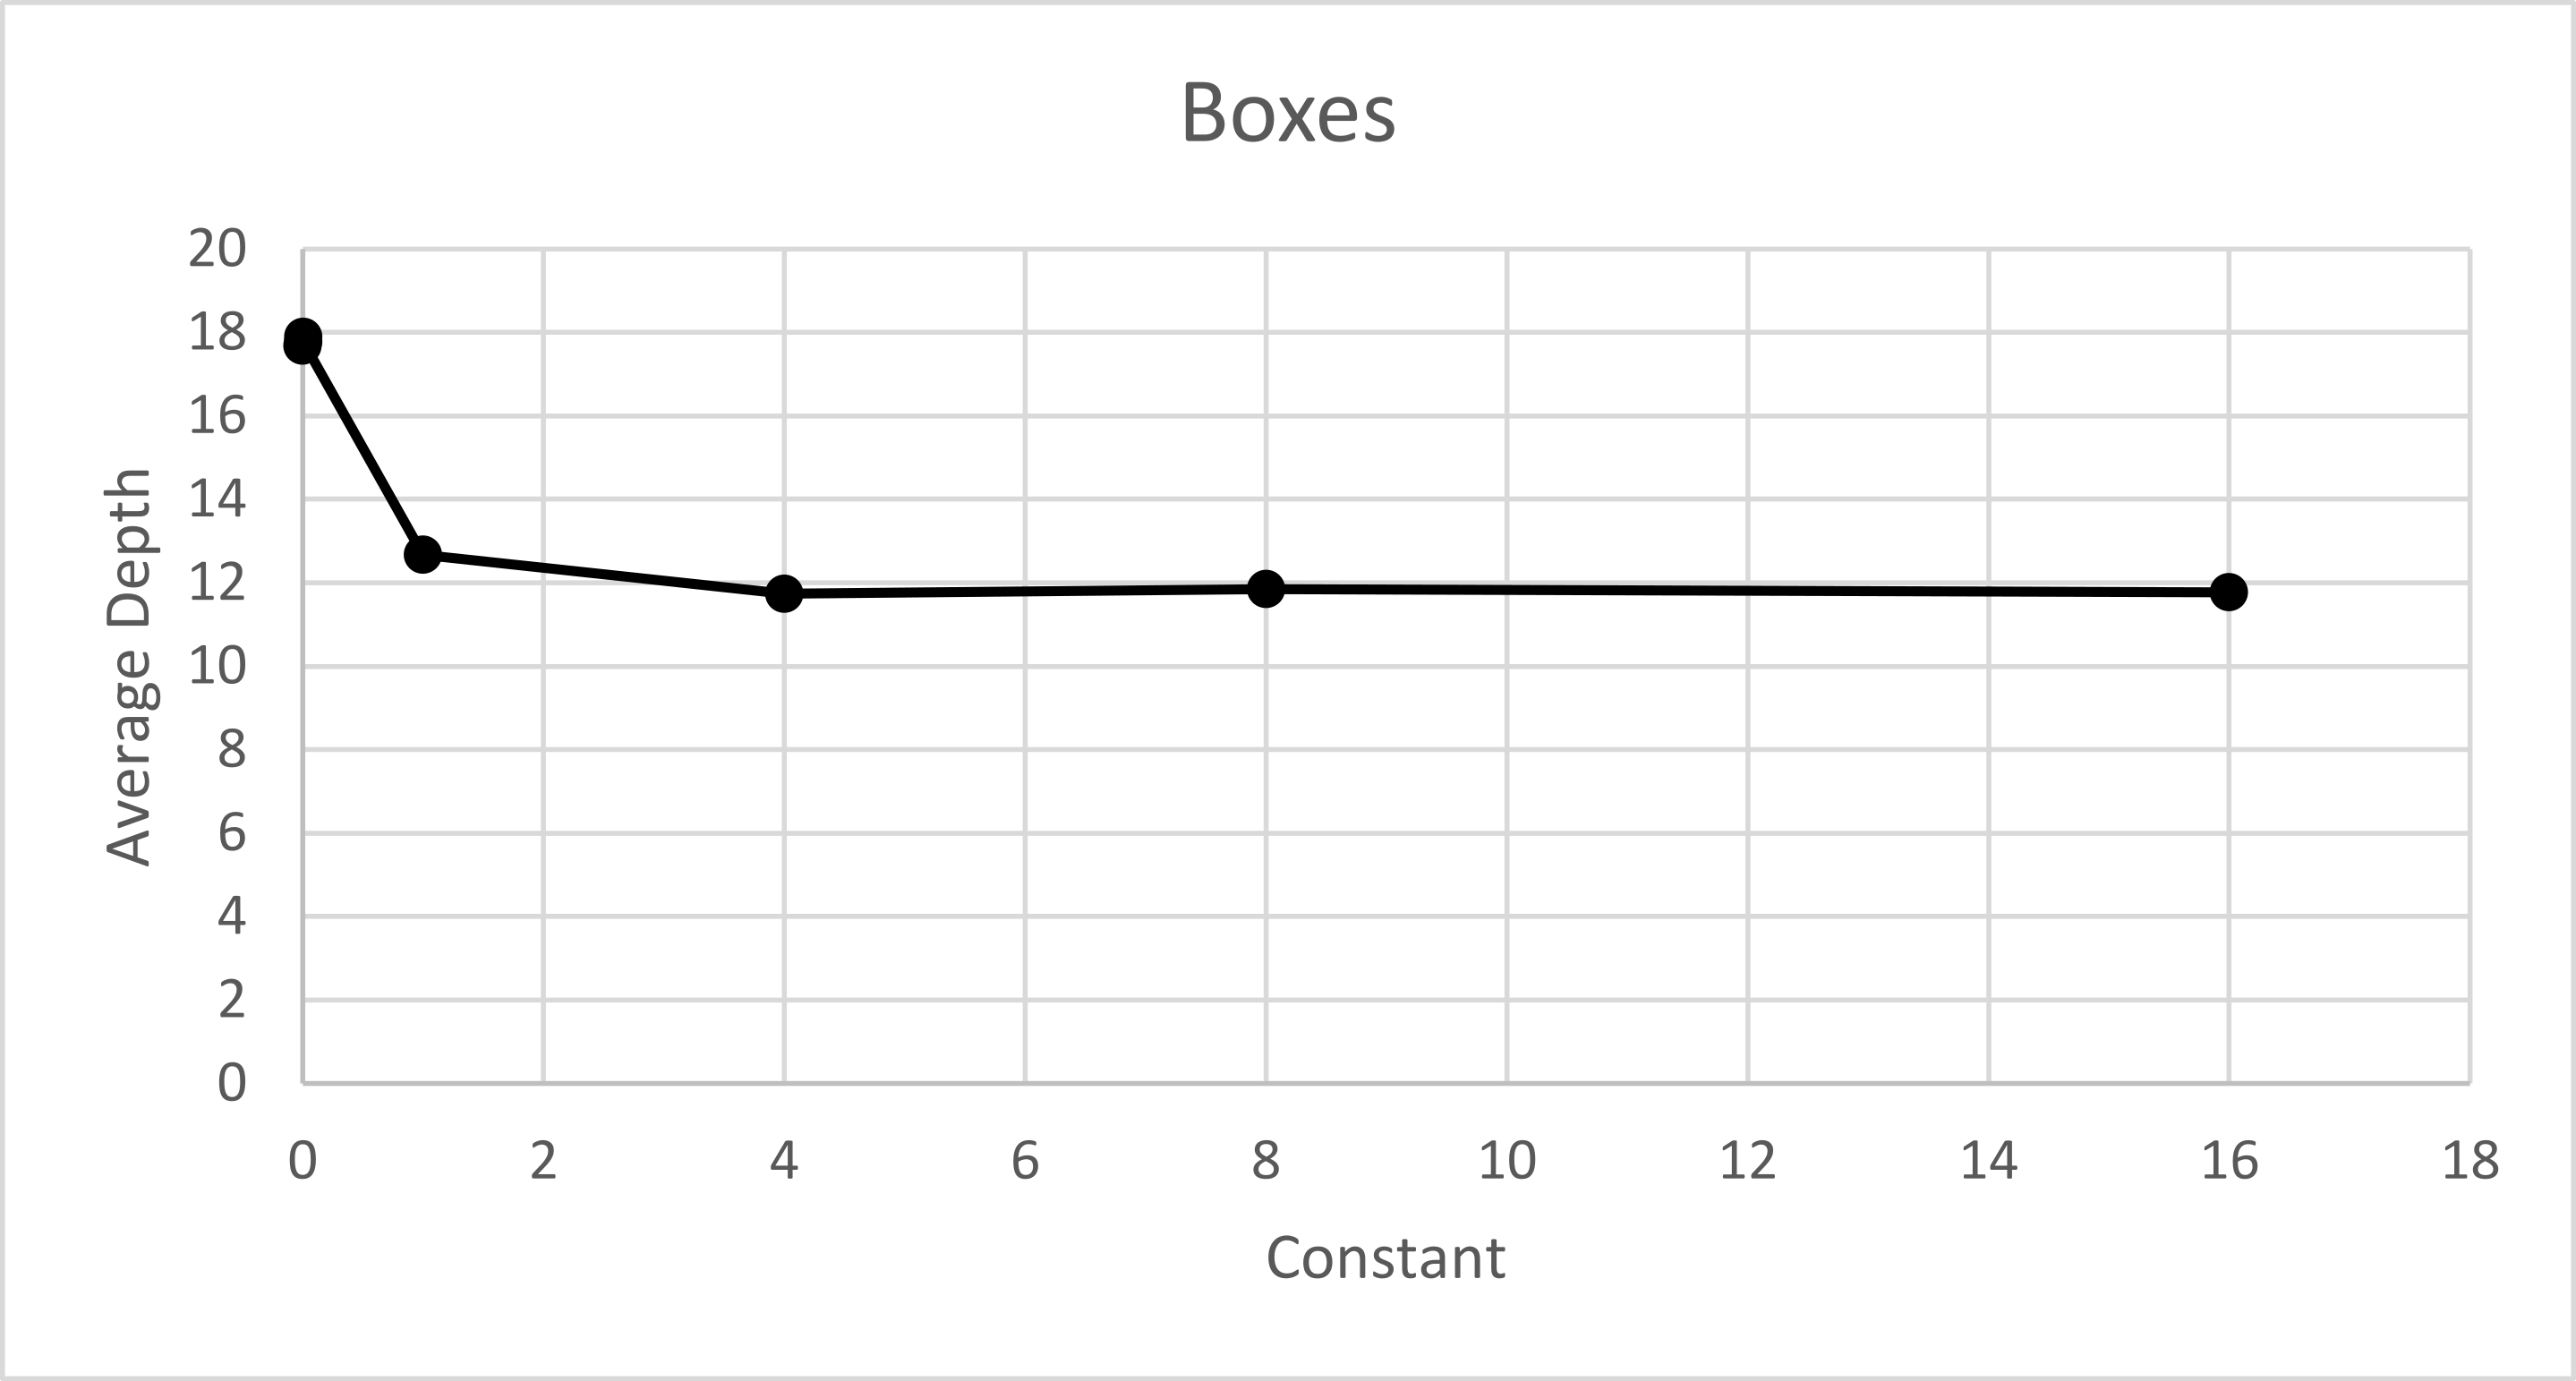
\includegraphics[width=0.8\linewidth]{pictures/BoxesDepth.png}}
\subfigure[Trend of solved levels rate using different constant values for reward Boxes]{
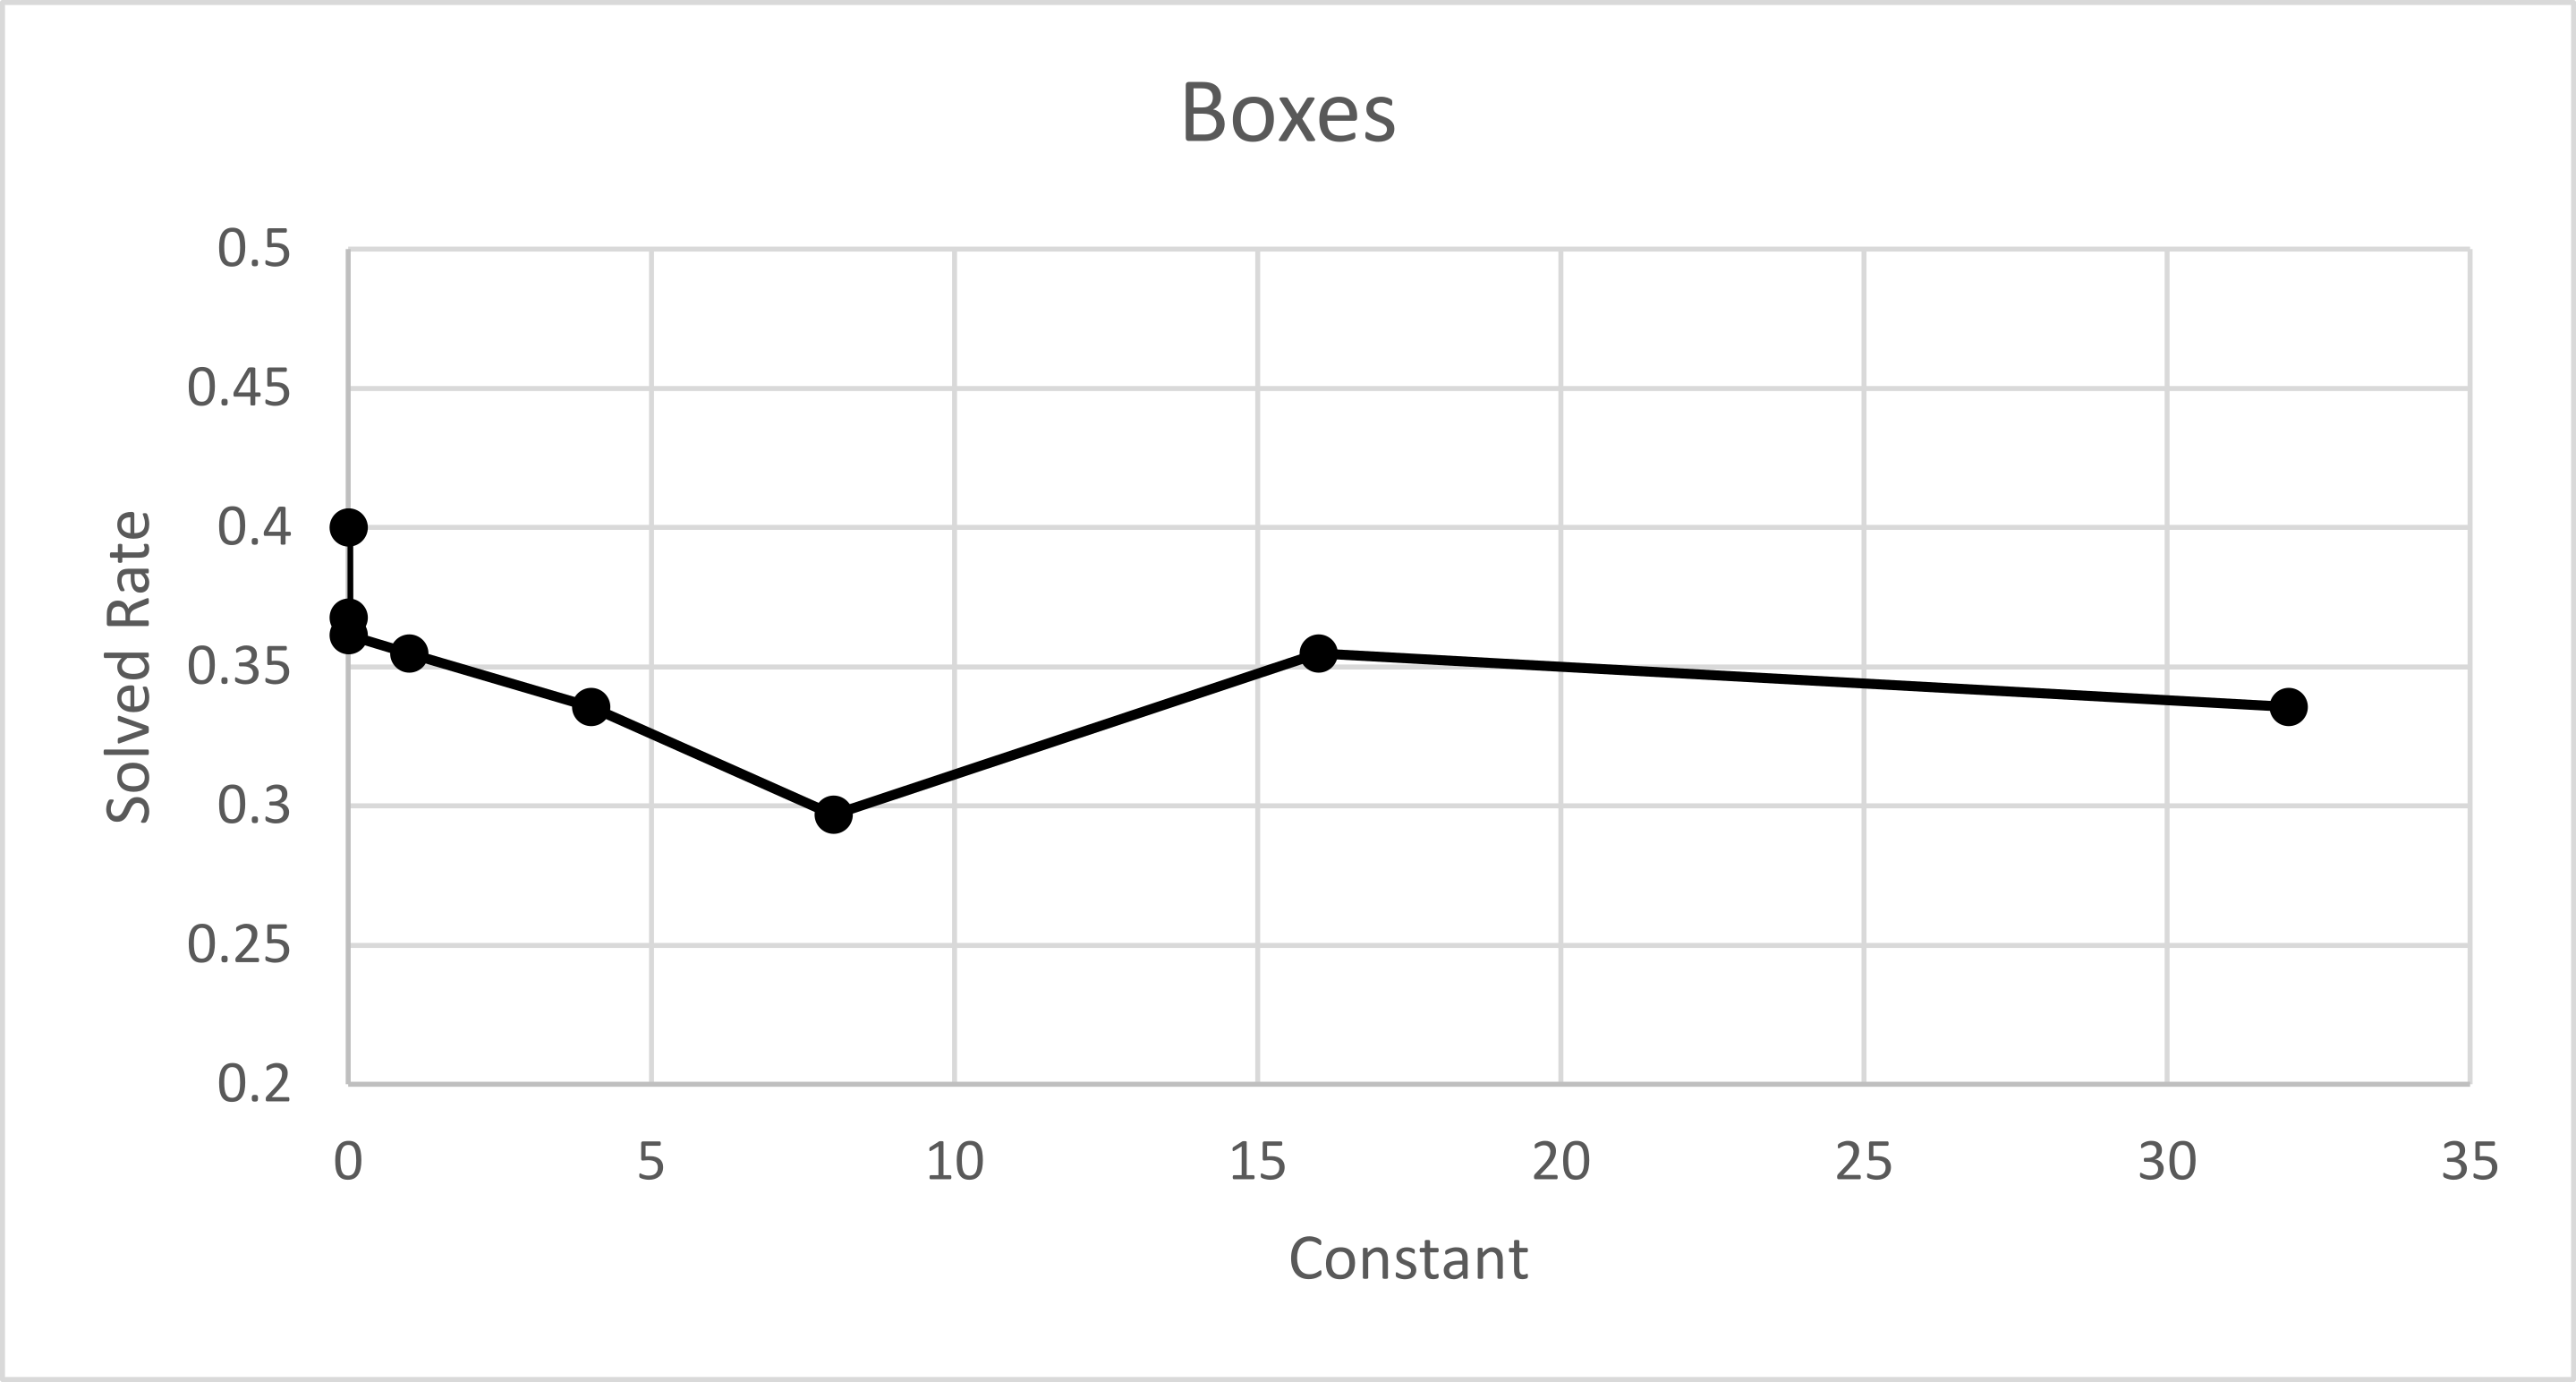
\includegraphics[width=0.8\linewidth]{pictures/BoxesSolved.png}}
\caption[Boxes solved levels rate and tree depth]{}
\label{fig:constant_Boxes}
\end{figure}

\medskip\noindent
The results using Boxes reward do not seem to follow a specific trend, and with the top score obtained with the constant equal to 0, this too does not appear to be suitable for solving Sokoban with MCTS.

\medskip\noindent
Considering these results, we selected NegativeBM as a reward for the following experiments.

\medskip\noindent
We also performed the same experiments using SP-MCTS and UCB1-Tuned to determine the best reward and constant configuration for each. The results are shown in Figures \ref{fig:spmcts_inverse} through \ref{fig:spmcts_R0}. SP-MCTS reached its peak performance with NegativeBM and a constant of 2, while UCB1-Tuned obtained the best result with InverseBM and a constant of 0.05.

\begin{figure}[!h]
    \centering
    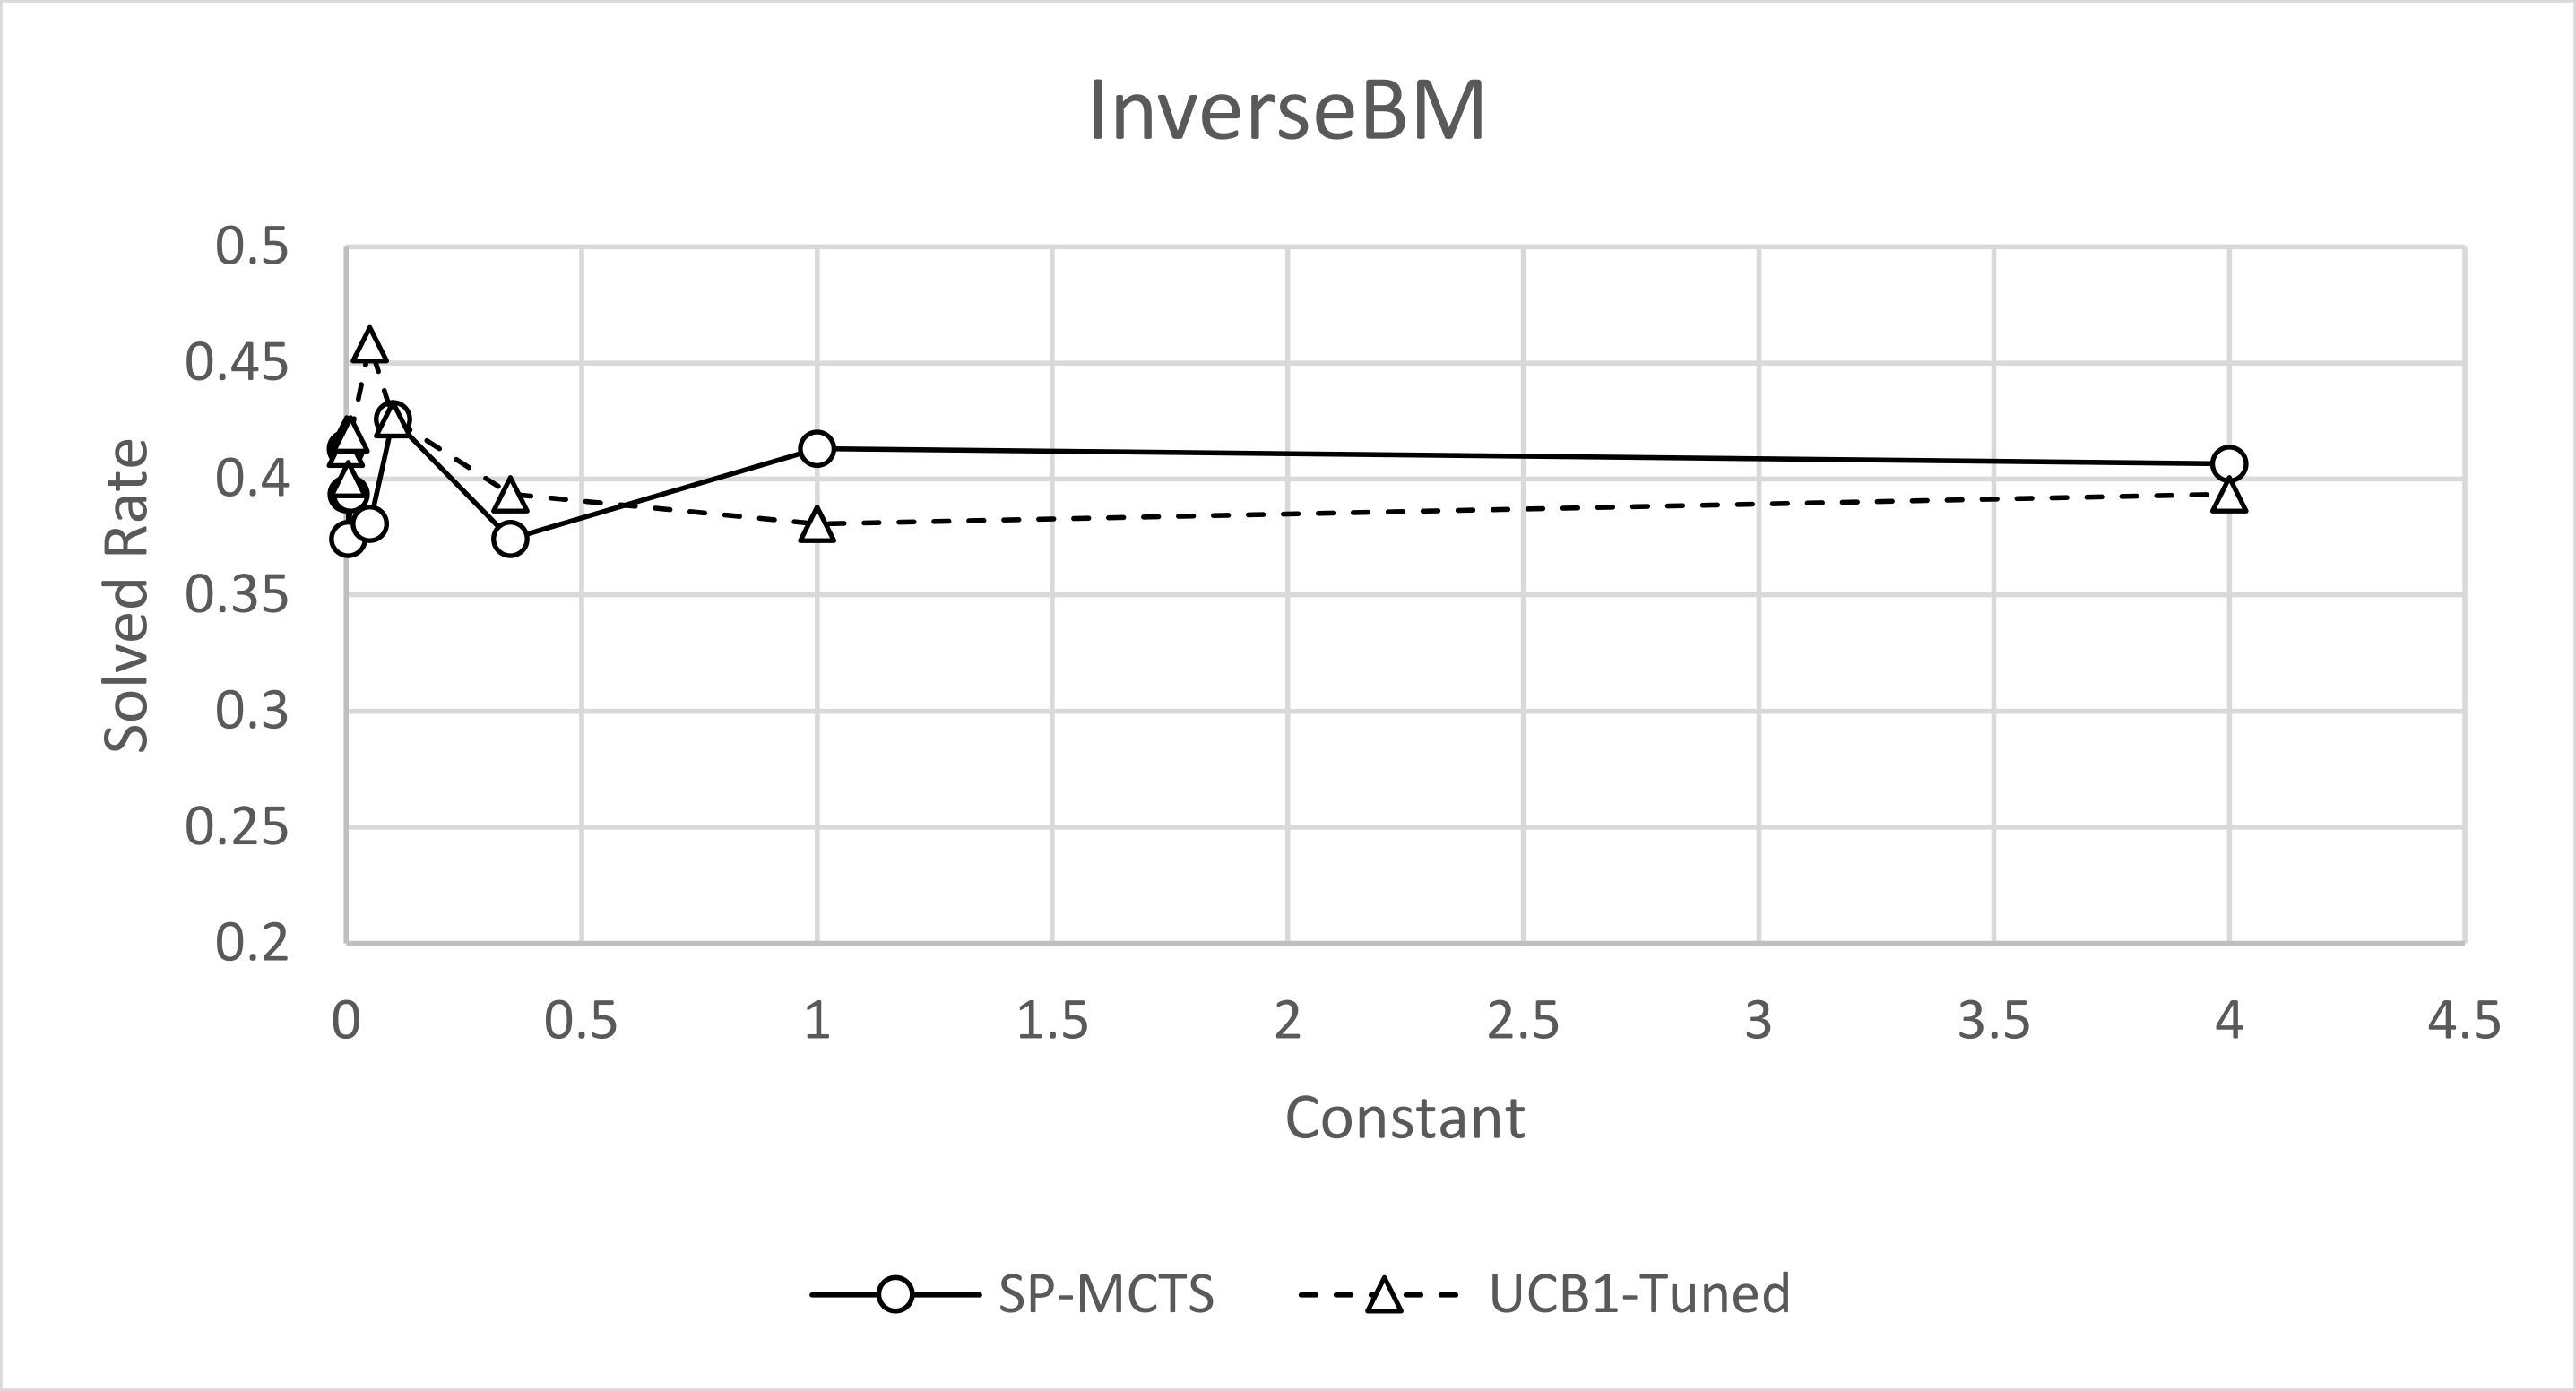
\includegraphics[width=0.8\linewidth]{pictures/Sokoban-SP-Inverse.png}
    \caption{SP-MCTS and UCB1-Tuned results with InverseBM}
    \label{fig:spmcts_inverse}
\end{figure}

\begin{figure}[!h]
    \centering
    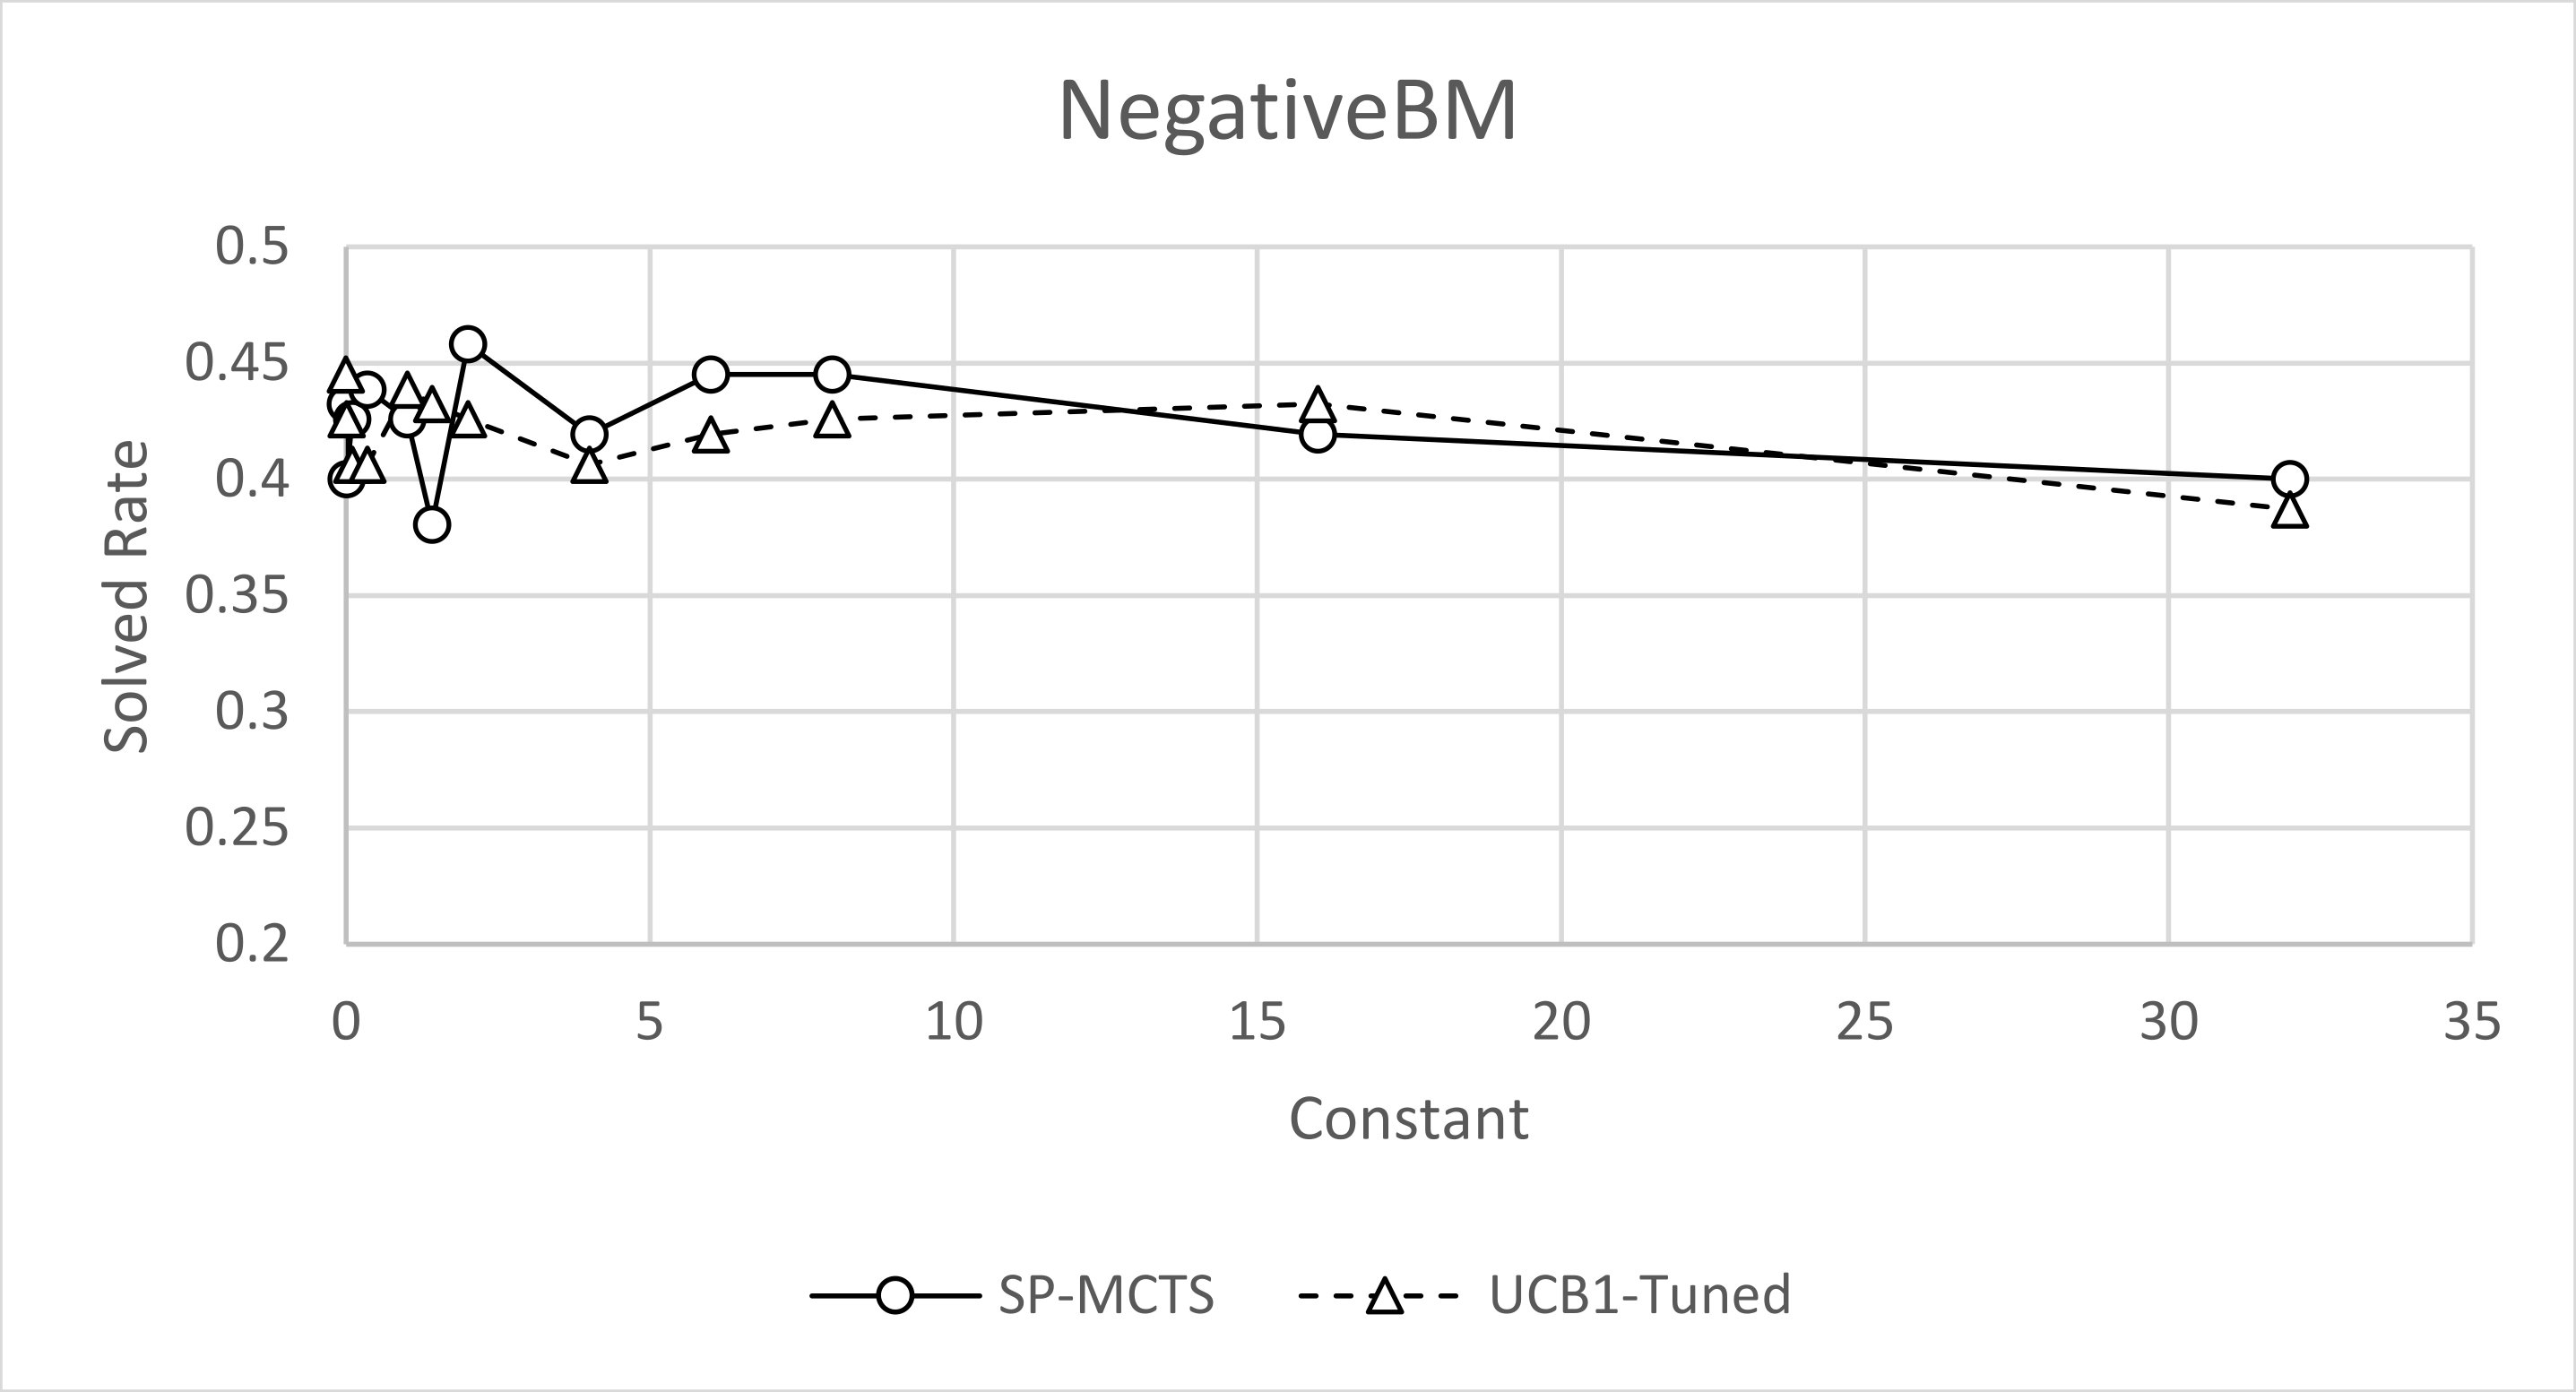
\includegraphics[width=0.8\linewidth]{pictures/Sokoban-SP-Negative.png}
    \caption{SP-MCTS and UCB1-Tuned results with NegativeBM}
    \label{fig:spmcts_negative}
\end{figure}

\clearpage

\begin{figure}[!h]
    \centering
    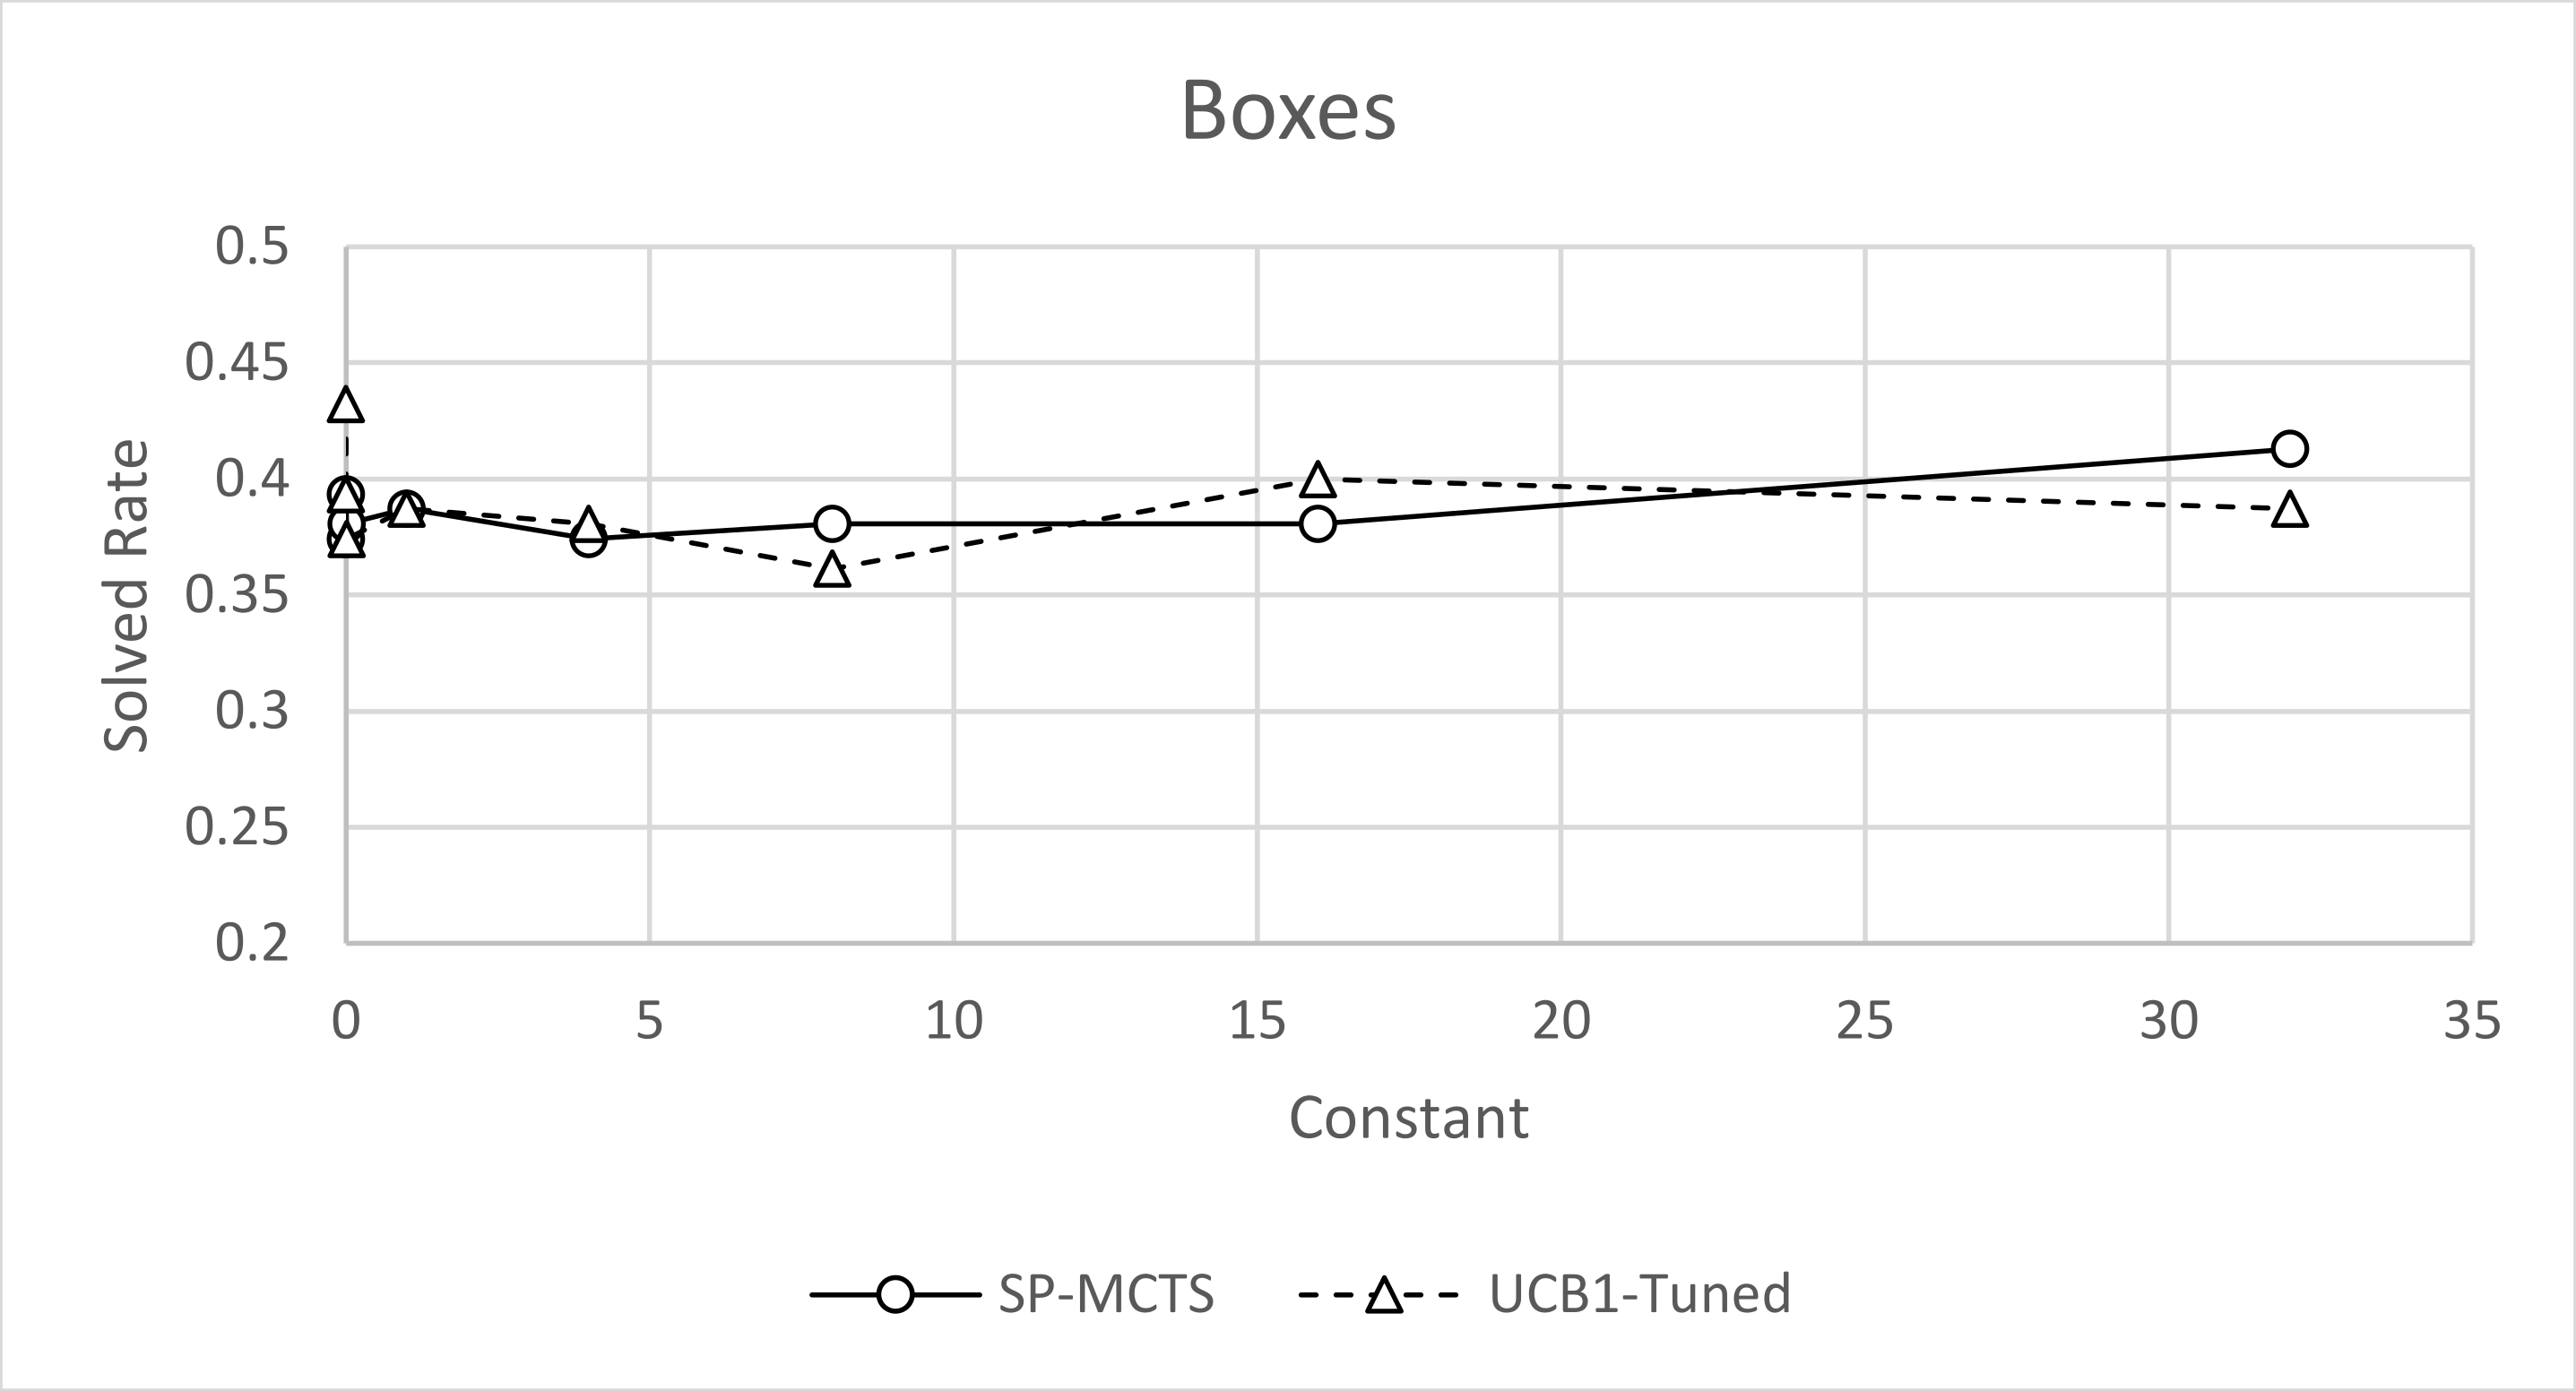
\includegraphics[width=0.8\linewidth]{pictures/Sokoban-SP-Boxes.png}
    \caption{SP-MCTS and UCB1-Tuned results with Boxes}
    \label{fig:spmcts_boxes}
\end{figure}

\begin{figure}[!h]
    \centering
    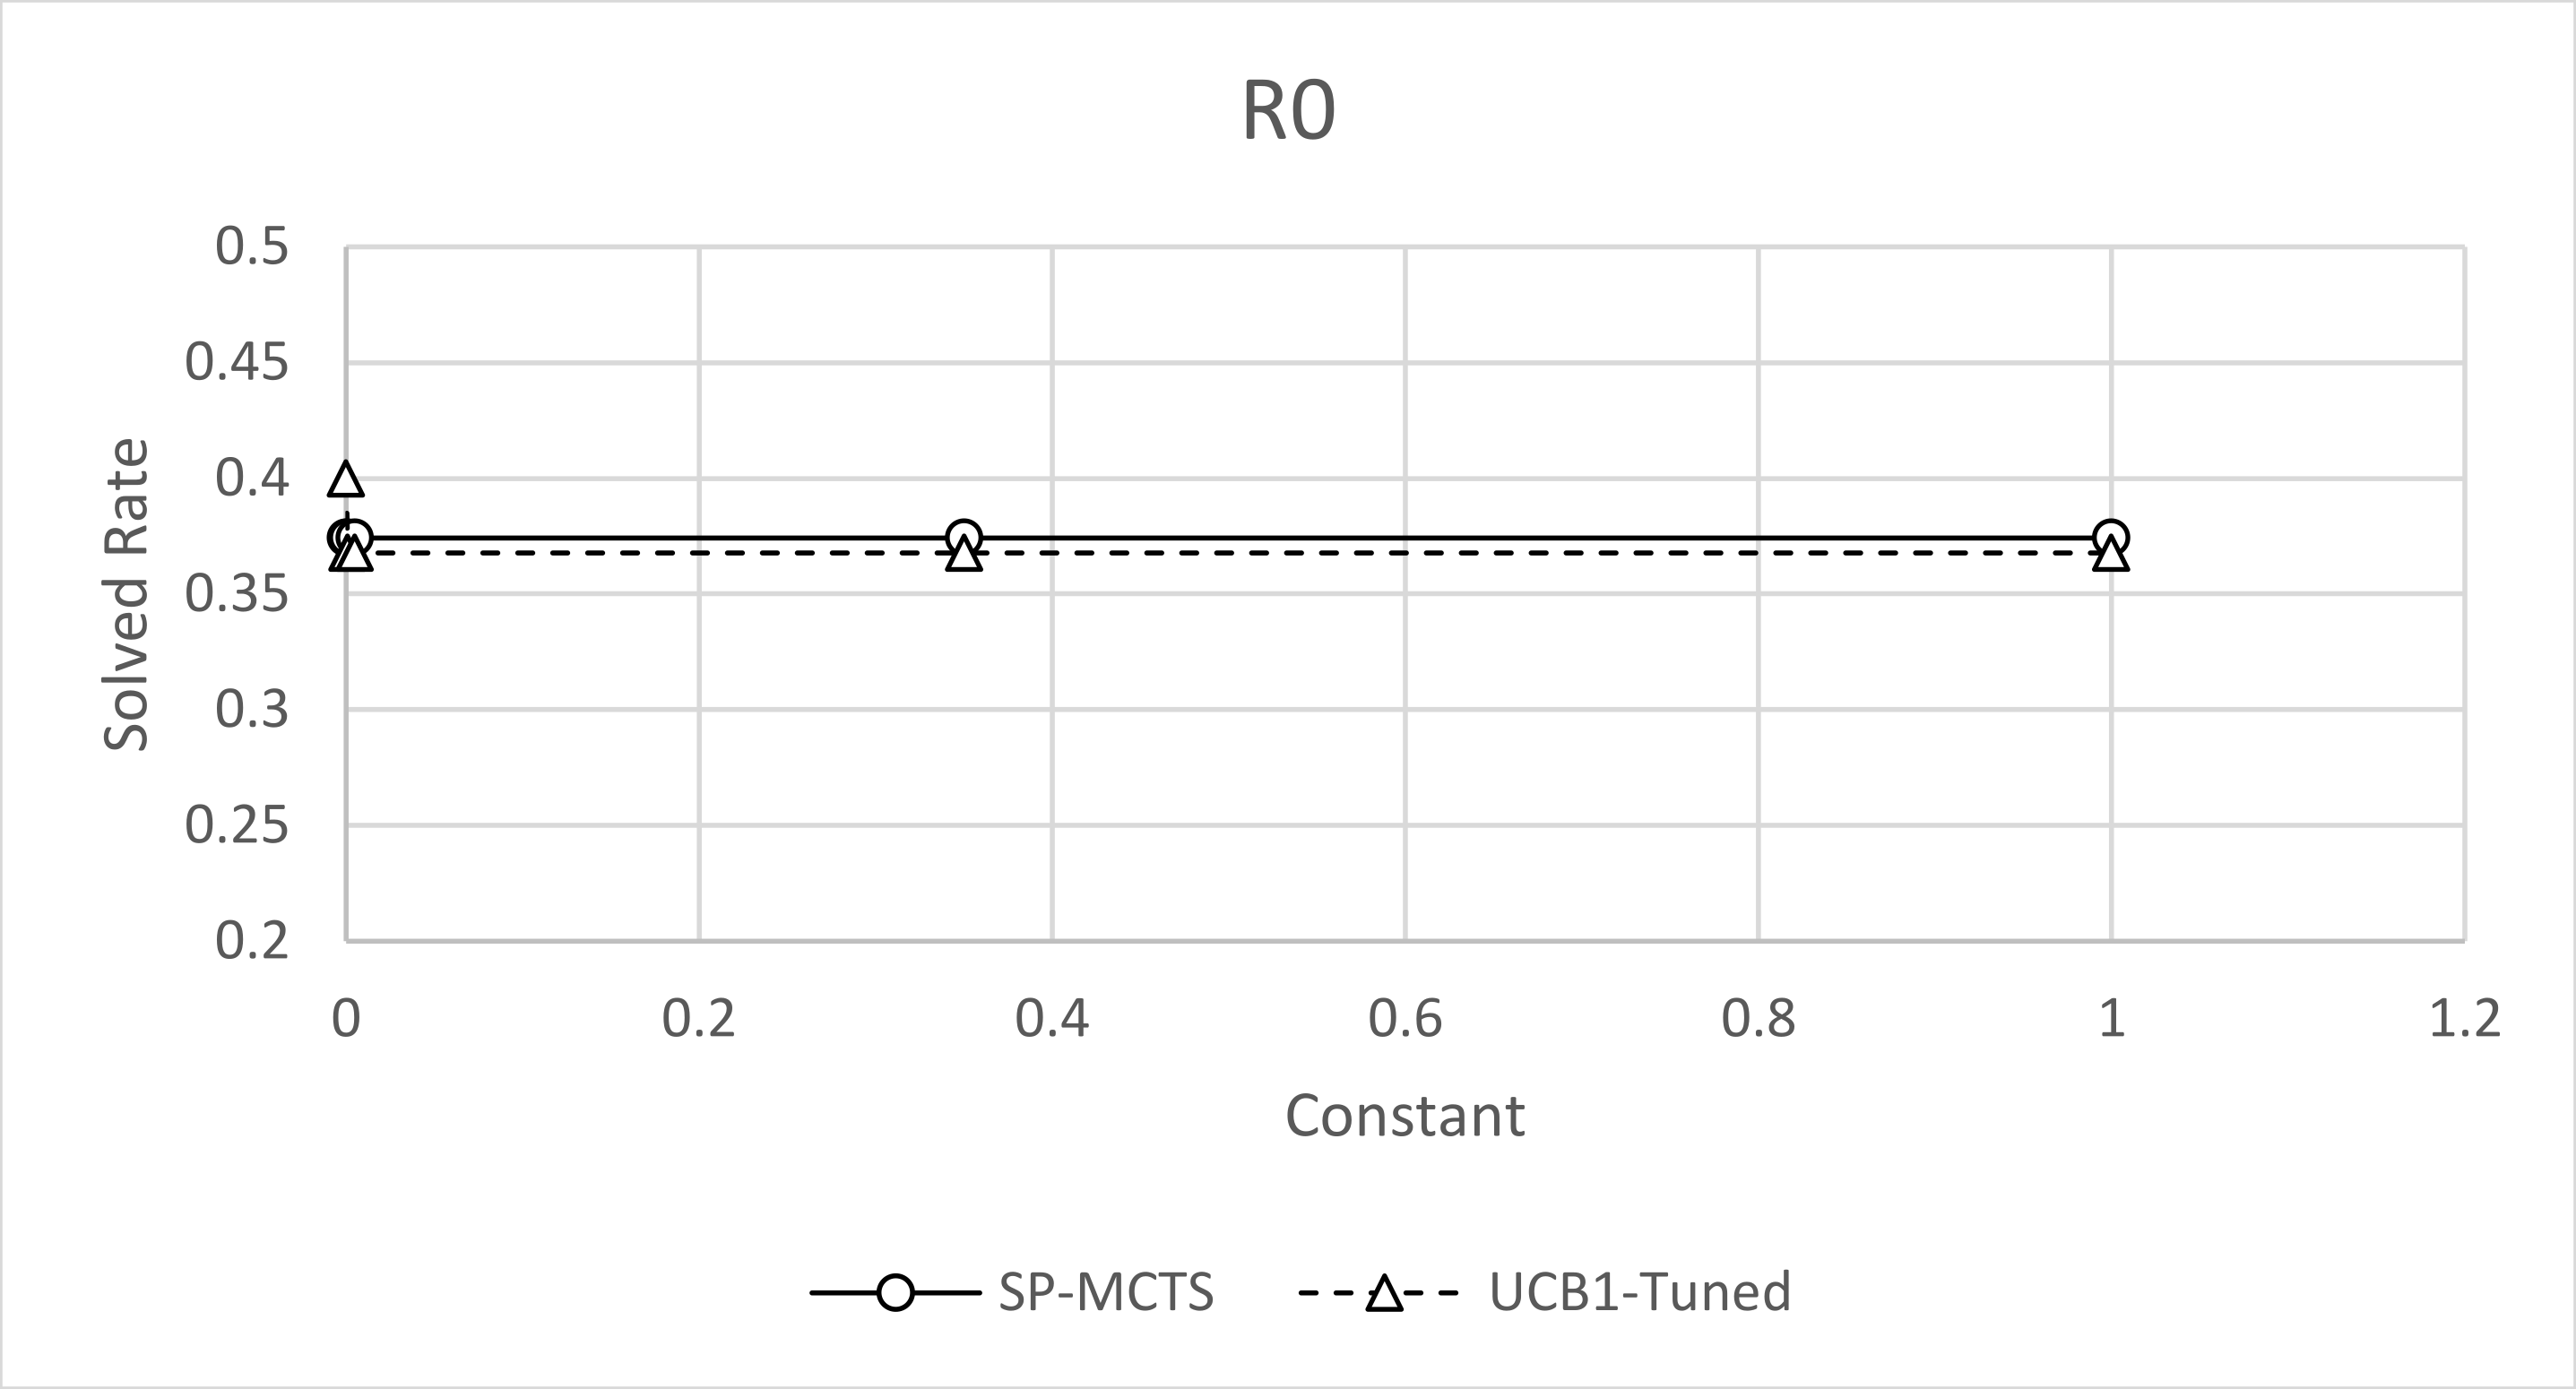
\includegraphics[width=0.8\linewidth]{pictures/Sokoban-SP-R0.png}
    \caption{SP-MCTS and UCB1-Tuned results with R0}
    \label{fig:spmcts_R0}
\end{figure}

\subsection{Node Elimination \& Cycles Avoidance}
In the following experiment we evaluated the effects of the Node Elimination and Cycles Avoidance optimizations. The baseline was obtained with standard UCT, random simulations, Node Elimination disabled and Cycles Avoidance in Stop On Cycle mode (i.e. the iteration is stopped if a cycle is detected).
\begin{figure}[!h]
    \centering
    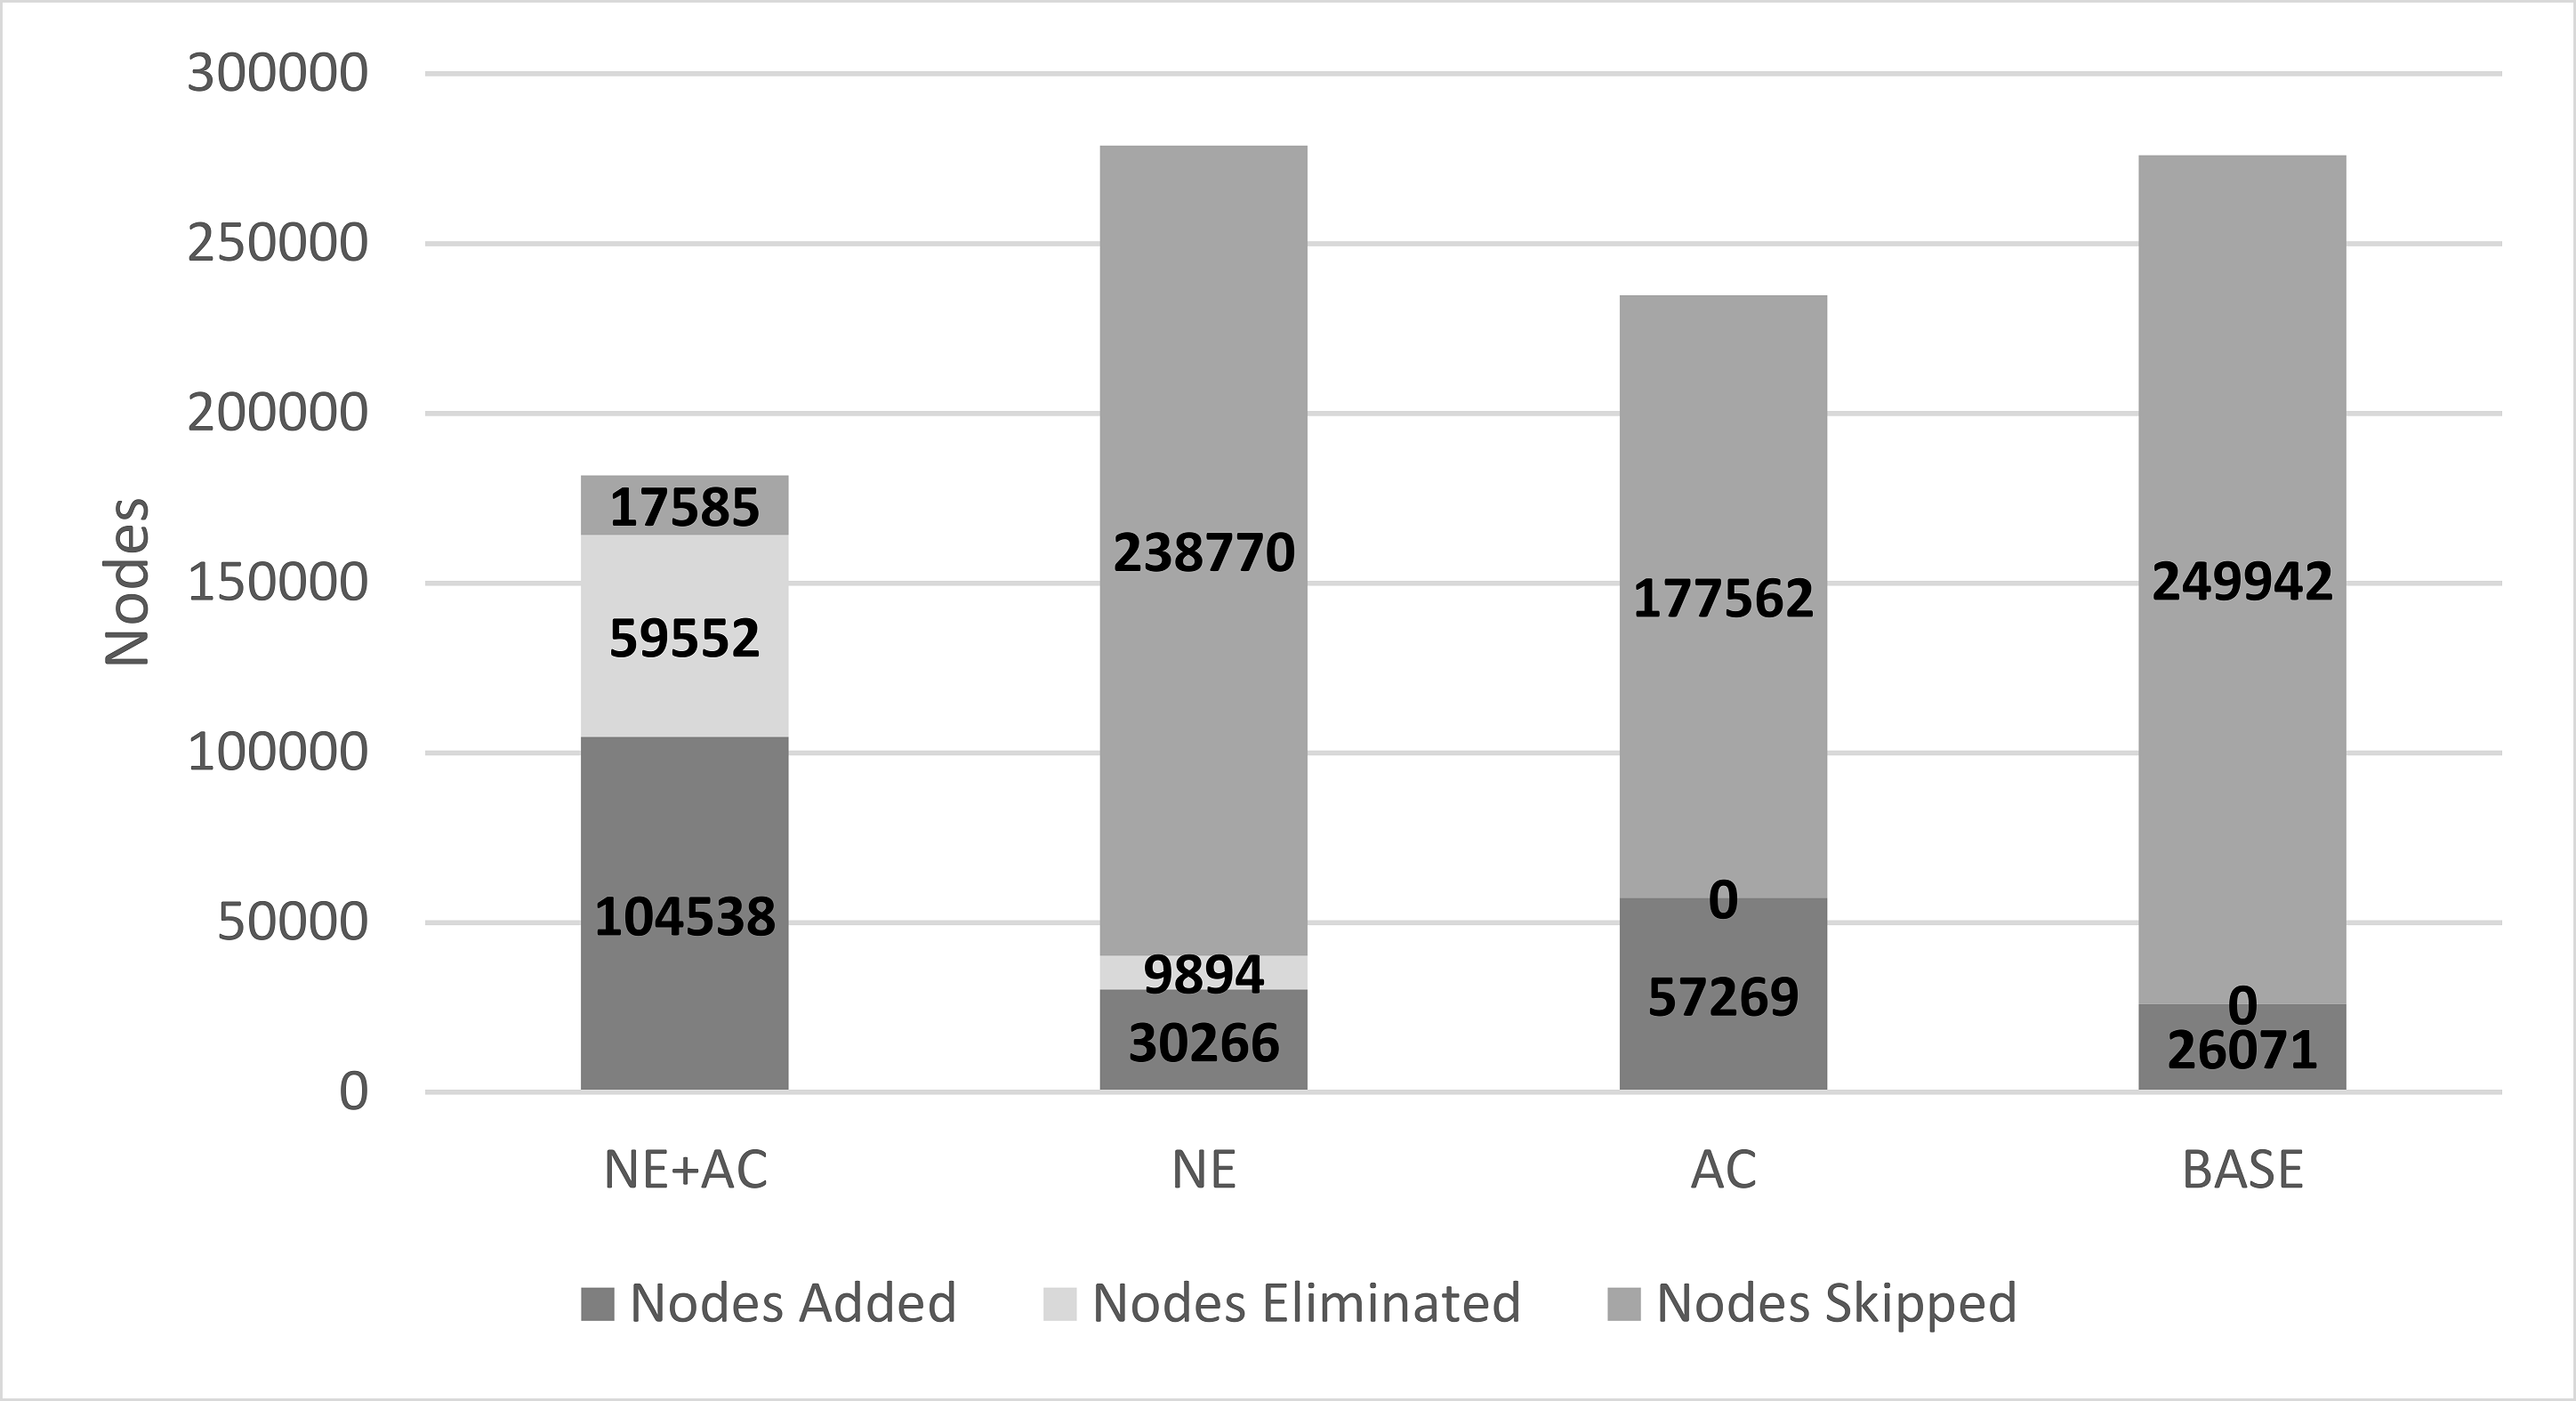
\includegraphics[width=0.9\linewidth]{pictures/SokobanNEACNodes.png}
    \caption[Node Elimination evaluation]{Nodes added, removed or skipped with combinations of Node Elimination (NE) and Avoid Cycles (AC)}
    \label{fig:SokobanNodeEliminationNodes}
\end{figure}

\medskip\noindent
Figure \ref{fig:SokobanNodeEliminationNodes} shows the number of nodes added to the search tree, the number of nodes deleted by Node Elimination and the number of iterations in which the expansion phase was skipped because the last selected node was terminal (nodes skipped). \textit{BASE} represents the baseline. We can see in Table \ref{tab:SokobanNodeEliminationNodes} how in the baseline the great majority of the iterations were executed without expanding the tree, thus terminating either on a cycle or on terminal nodes. Node Elimination prevented the algorithm from revisiting terminal nodes, causing it to slightly increase the number of nodes added to the tree, but its impact on the number of solved levels was not positive. The Avoid Cycles mode of Cycle Avoidance lead to a larger increase in the number of expanded nodes, when compared to Node Elimination. The increase in number of solved levels also lead to a decrease in the total number of iterations (as the search is stopped as soon as a solution is found). The combination of Node Elimination and Avoid Cycles obtained the best results, with far more nodes added to the tree and the highest number of solved levels.

\begin{table}[!h]
    \centering
    \begin{tabular}{l|l|l|l|l}
        Configuration & Added & Eliminated & Skipped & Solved\\
        Baseline & 9\% & 0\% & 91\% & 20\\
        Node Elimination & 11\% & 3\% & 86\% & 18\\
        Avoid Cycles & 24\% & 0\% & 76\% & 44\\
        NE + AC & 57\% & 33\%  & 10\% & 76
    \end{tabular}
    \caption[Node Elimination and Avoid Cycles evaluation]{Percentages of nodes added, eliminated and skipped, along with the number of solved levels for each configuration. The last row represents the combination of Node Elimination and Avoid Cycles}
    \label{tab:SokobanNodeEliminationNodes}
\end{table}

\medskip\noindent
Figure \ref{fig:SokobanNodeEliminationSolved} illustrates the performance of the different configurations with various number of iterations.

\begin{figure}[!h]
    \centering
    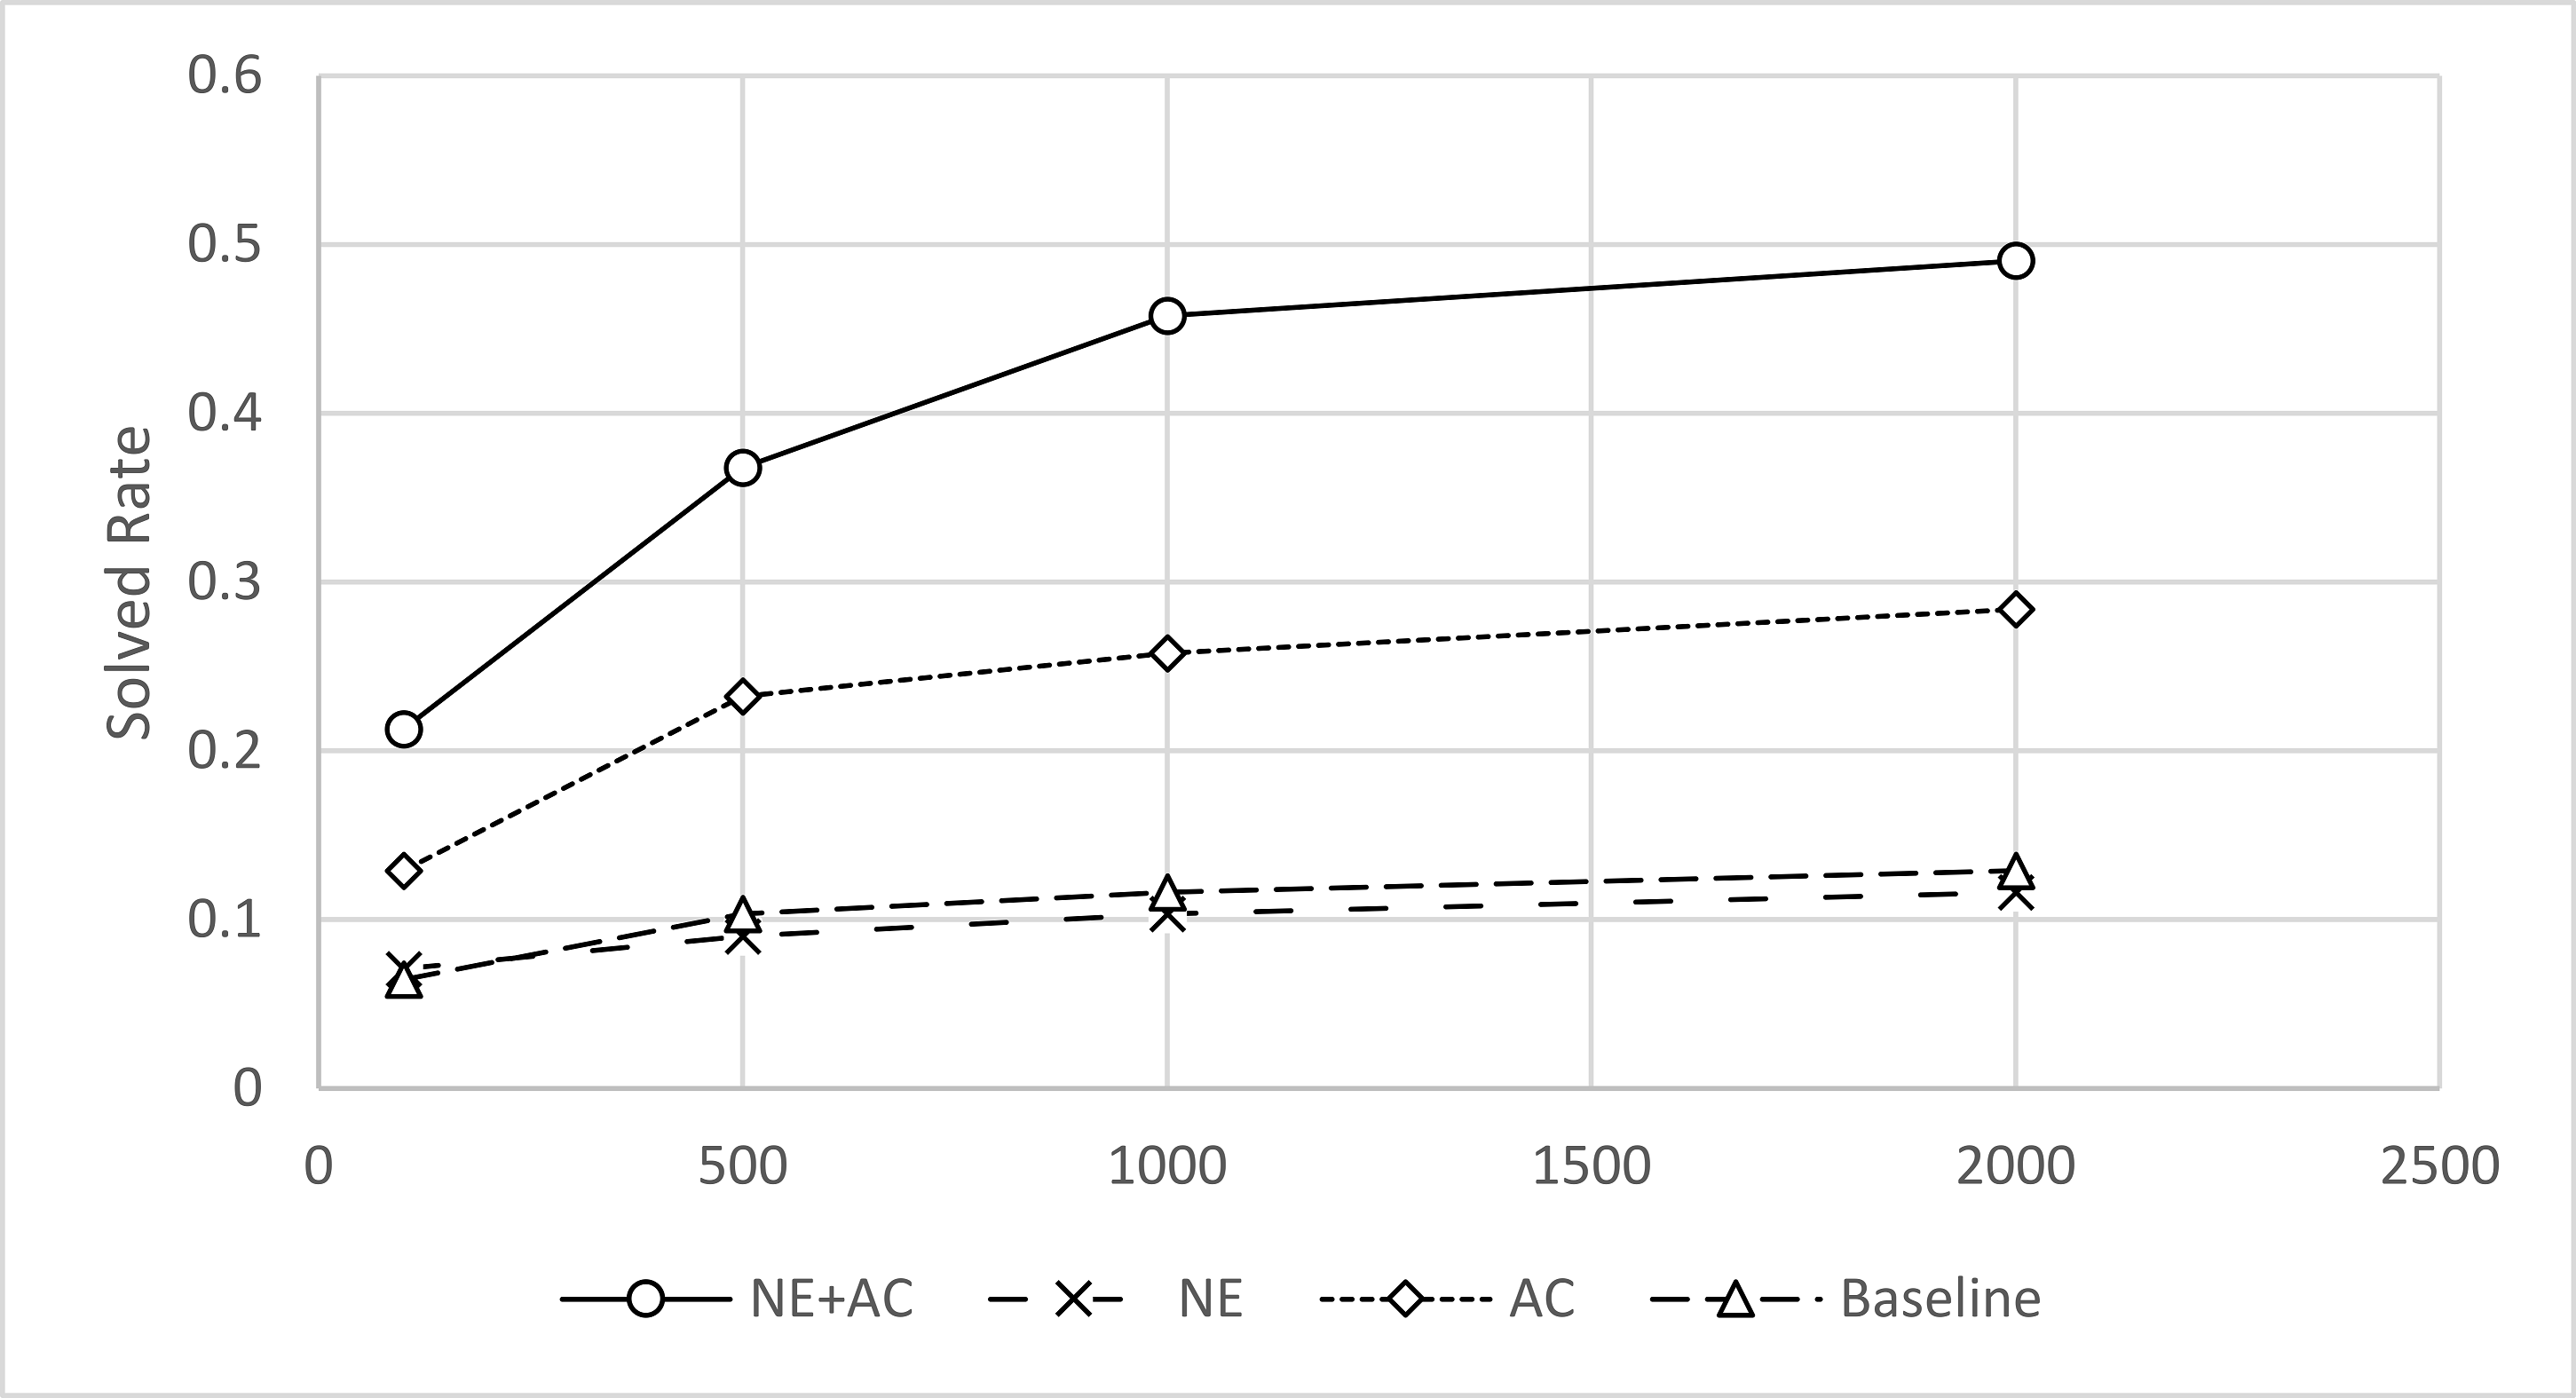
\includegraphics[width=0.9\linewidth]{pictures/SokobanNEACSolved.png}
    \caption[Node Elimination and Avoid Cycles solved levels]{Solved levels with combinations of Node Elimination (NE) and Avoid Cycles (AC) and different number of iterations}
    \label{fig:SokobanNodeEliminationSolved}
\end{figure}
\clearpage

\subsection{Parameters tuning}
\medskip\noindent
Then we tested all MCTS optimizations separately, as we done for Samegame, in order to determine the effect of each one on Sokoban and, after that, we combined all the enhancement together, trying to obtain the best result. Again we proceeded with the tuning of the parameters. In particular, we executed repeated searches with different values for the RAVE threshold and the memory budget of Node Recycling. Other enhancements such as UCB1Tuned and Node Elimination have no parameters, hence they do not require tuning.

\medskip\noindent
Table \ref{tab:sokoban_tuningrave} shows variation in term of performance on the test set as the parameter $V$ change; this parameter represents the maximum number of visits a node needs to have before the RAVE values are not used at all.

\begin{table}[!h]
    \centering
    \begin{tabular}{l|l}
        V & Solved \\
        \hline 
        1 & 45.8 \% \\
        5 & 41.9 \% \\
        10 & 42.6 \% \\
        15 & 41.9 \% \\
        25 & 42.6 \% \\
        50 & 43.8 \% \\
        100 & 42.6 \% \\
    \end{tabular}
    \caption[RAVE thresholds evaluation]{Levels solved with different RAVE thresholds. The first row is equivalent to disabling RAVE and represents our baseline.}
    \label{tab:sokoban_tuningrave}
\end{table}

\medskip\noindent
With the exception of $V=1$, which is equivalent to disabling RAVE, we can see that RAVE solved the highest number of levels with $V = 50$. However the performance was still lower than the baseline. As we did for Samegame, we concluded that the assumption necessary for RAVE to perform well does not hold for Sokoban.

\medskip\noindent
Table \ref{tab:sokoban_tuningrecycling} shows instead performance trend on the test set changing the parameter responsible for the maximum number of nodes kept in memory by the Node Recycling optimization; this parameter is used as memory budget parameter in order to keep in memory only the most promising nodes and recycling the less promising ones.
\begin{table}[!h]
    \centering
    \begin{tabular}{l|l}
        Nodes & Solved \\
        \hline 
        200 & 43.2 \% \\
        400 & 43.2 \% \\
        600 & 43.2 \% \\
        800 & 43.2 \% \\
        1000 & 45.8 \% \\
    \end{tabular}
    \caption[Node Recycling memory budgets evaluation]{Levels solved with Node Recycling and different memory budgets. The last row is equivalent to disabling Node Recycling and represents our baseline.}
    \label{tab:sokoban_tuningrecycling}
\end{table}
We can see how independently of the memory budget, Node Recycling performed uniformly worse than the baseline in Sokoban.

\subsection{Simulation policy}
\medskip\noindent
Next we tested different options for the simulation policy: we performed searches using random simulations, $\epsilon$-greedy and $\epsilon$-IDA* with different combinations of IDA* nodes and MCTS iterations. Since the IDA* simulations were significantly heavier than random and $\epsilon$-greedy ones, we compared the policies on similar execution times. The value of $\epsilon$ was set to 0.2 for both $\epsilon$-based policies. Table \ref{tab:hybridpolicies} shows the results of the various $\epsilon$-IDA* configurations. Table \ref{tab:simulationpolicies} shows the comparison between $\epsilon$-IDA*, $\epsilon$-greedy and random simulation policies. $\epsilon$-greedy solved 95 levels

\begin{table}[!h]
    \centering
    \begin{tabular}{ l | l | l | l }
        IDA* Nodes & MCTS Iterations & Time & Solved \\
        \hline
        100 & 100 & 1h 13m 21s & 55.5\% \\
        20 & 500 & 1h 28m 30s & 54.2\% \\
        5 & 1000 & 1h 0m 50s & 54.2\% \\
    \end{tabular}
    \caption[Results of $\epsilon$-IDA*]{Results of $\epsilon$-IDA*. Each row represents one configuration.}
    \label{tab:hybridpolicies}
\end{table}


\begin{table}[!h]
    \centering
    \begin{tabular}{l|l|l|l}
        Policy & Iterations & Time & Solved \\
        \hline
        $\epsilon$-IDA*(100) & 100 & 1h 13m 21s & 55.5\%\\
        $\epsilon$-greedy & 5000 & 1h 9m 47s & 61.3\% \\
        Random & 5000 & 1h 11m 55s & 52.3\% \\
    \end{tabular}
    \caption{Results of the different simulation policies.}
    \label{tab:simulationpolicies}
\end{table}

\subsection{Sokoban complexity}
During our experiments we noticed that contrary to what we expected, the performance of MCTS didn't improve much when increasing the number of iterations. When comparing the number of levels solved relative to the number of nodes used in IDA* and the number of iterations performed in MCTS, we noticed a similar trend (Figures \ref{fig:sokobanIDAComplexity} and \ref{fig:sokobanMCTSComplexity}). After reaching a certain threshold, the resources needed to solve additional levels increase dramatically. We consider this to be a consequence of the quality of the heuristic evaluation which is not suitable for levels in which boxes must be pushed away from goals in order to find a solution. It's still not clear why the threshold in MCTS appears earlier than in IDA*.

\begin{figure}[!h]
    \centering
    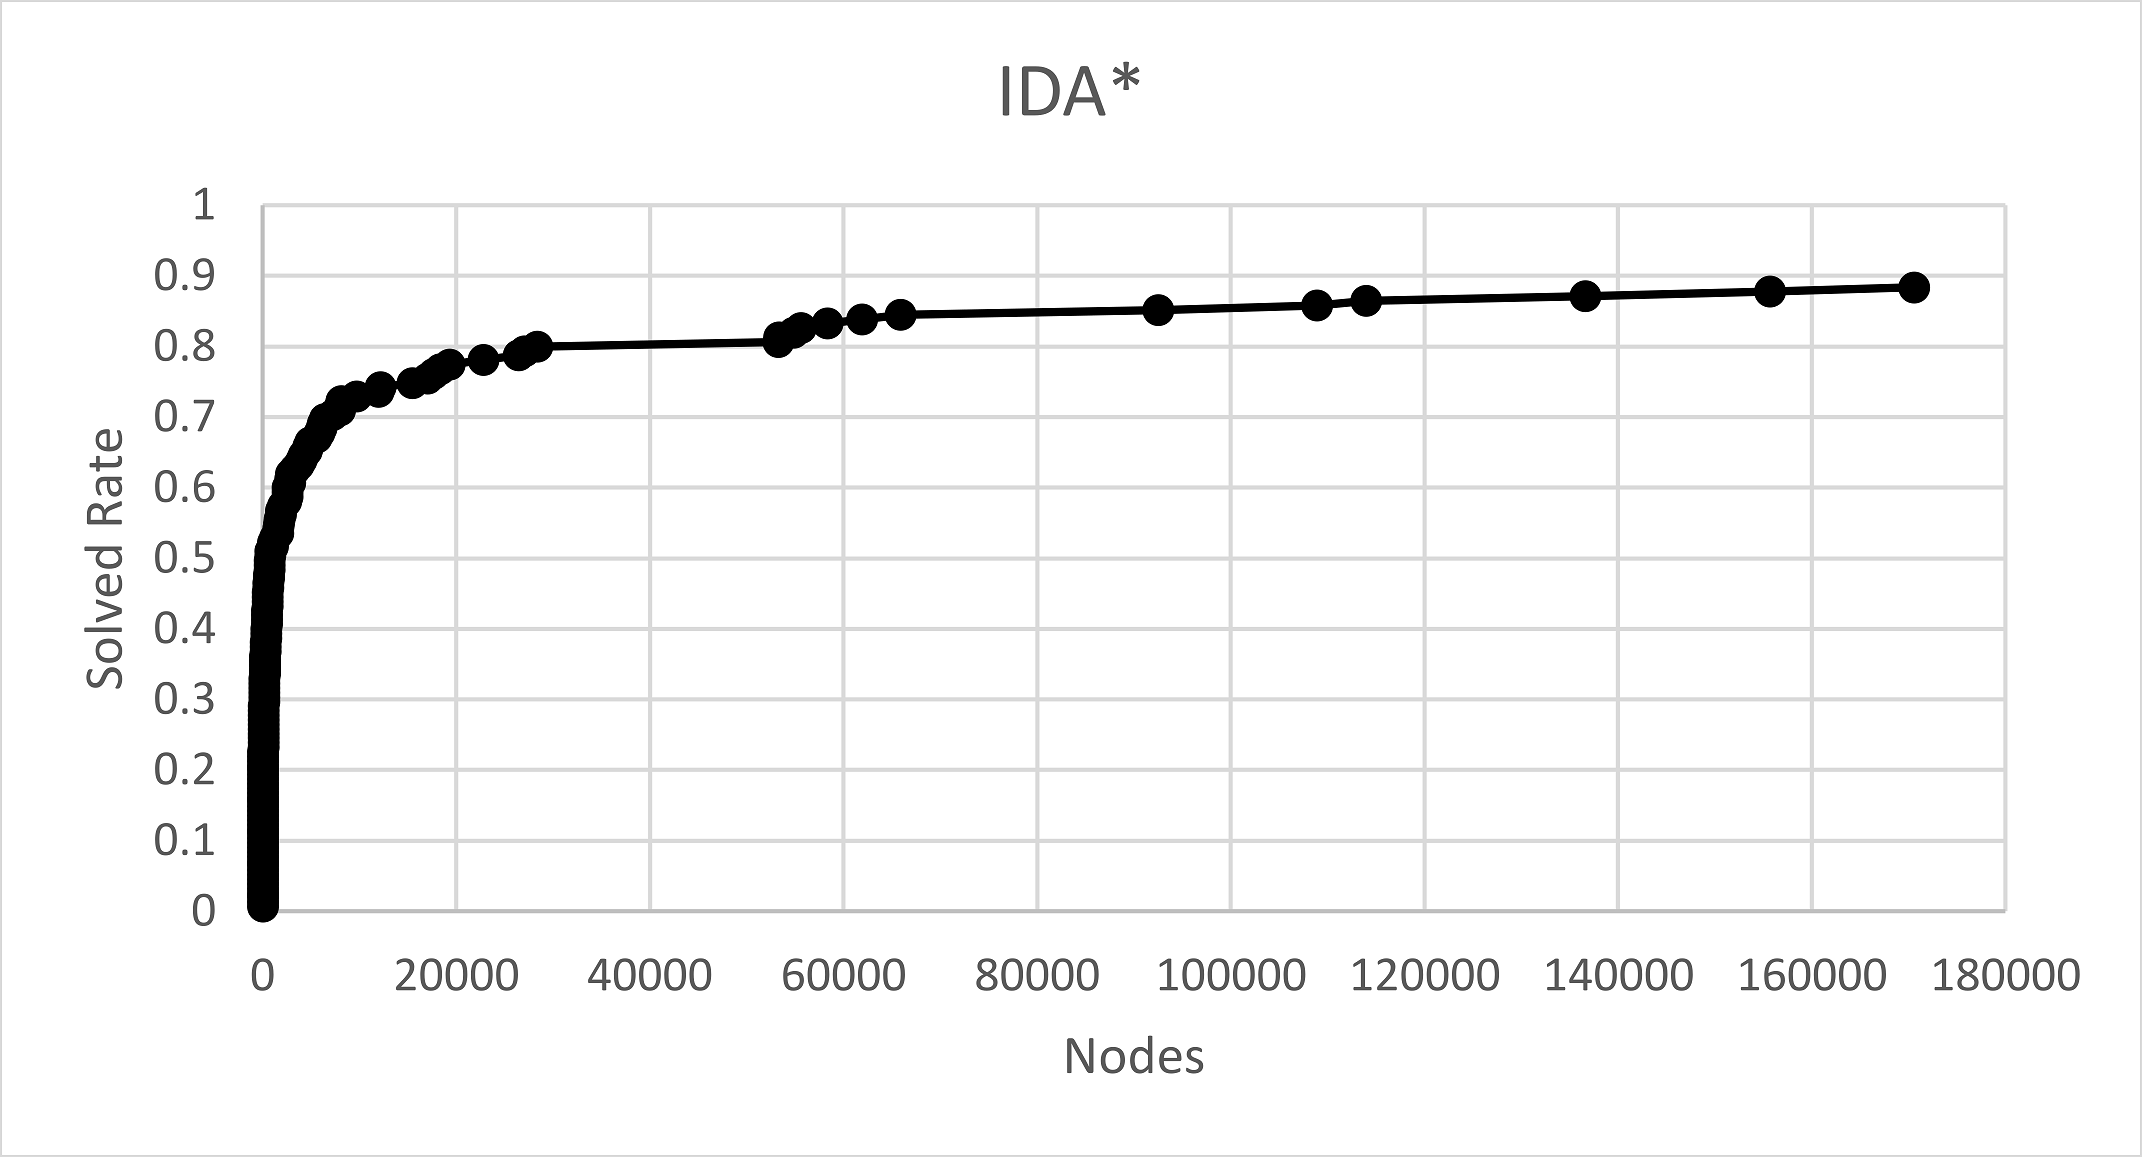
\includegraphics[width=0.8\linewidth]{pictures/SokobanIDAComplexity.png}
    \caption[IDA* solved levels]{Levels solved according to number of nodes used in IDA*}
    \label{fig:sokobanIDAComplexity}
\end{figure}
\clearpage

\begin{figure}[!h]
    \centering
    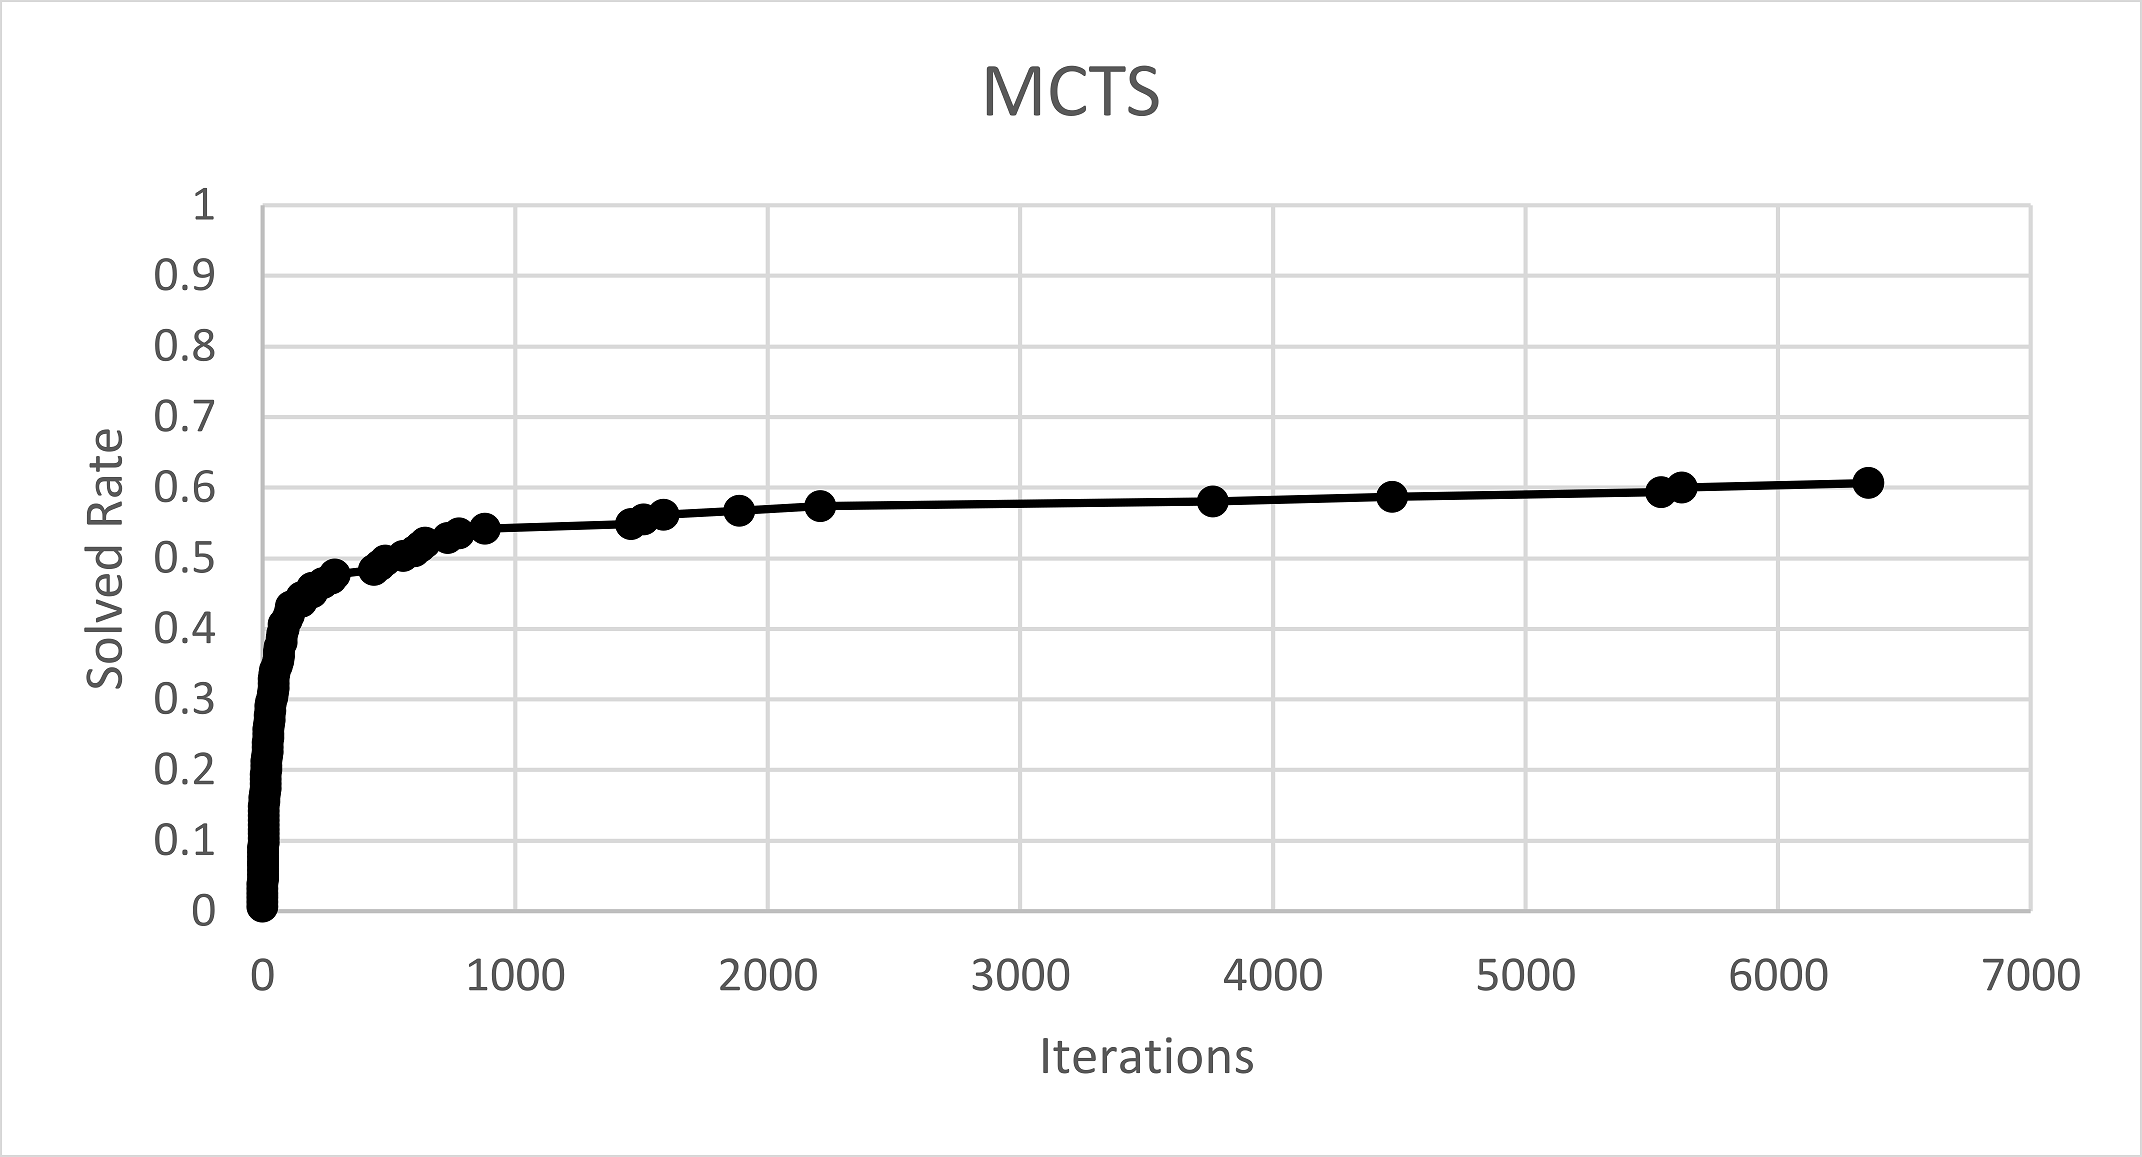
\includegraphics[width=0.8\linewidth]{pictures/SokobanMCTSComplexity.png}
    \caption[MCTS solved levels]{Levels solved according to number of iterations performed in MCTS}
    \label{fig:sokobanMCTSComplexity}
\end{figure}

\subsection{Results}
The last experiment we performed consisted in the comparison between IDA* and different versions of MCTS for Sokoban. For this final comparison we used three versions of MCTS based on the formula used for the estimation of the action-value function: standard UCT, UCB1-Tuned and SP-MCTS. Standard MCTS used NegativeBM as a reward with a constant of 6. UCB1-Tuned used InverseBM as a reward with a constant of 0.05. SP-MCTS used NegativeBM as a reward, with a constant of 2. Node Elimination and Cycles Avoidance were enabled in all three configurations. To keep a comparable search time between all methods, IDA* used a maximum of 200000 nodes and all MCTS methods used 10000 iterations with $\epsilon$-greedy as a simulation policy, with $\epsilon=0.2$. Table \ref{tab:sokoban_results} shows the final results of this comparison.
\begin{table}[!h]
    \centering
    \begin{tabular}{l|l}
        Method & Solved \\
        \hline
        IDA* & 88.4\%\\ 
        UCT & 64.5\%\\
        UCB1-Tuned & 54.8\%\\
        SP-MCTS & 60.6\%\\
    \end{tabular}
    \caption{Methods comparison}
    \label{tab:sokoban_results}
\end{table}
\clearpage
\medskip\noindent
IDA* solved the highest number of levels with respect to the other methods. Among MCTS methods, UCT achieved the best performance with 64.5\% of solved levels.
\chapter{Conclusions}
\label{results}
The purpose of this thesis was to measure the performance of MCTS in Sokoban. We developed various optimizations for MCTS and verified their effectiveness on Sokoban and Samegame. RAVE obtained poor results in both domains and we concluded that neither Sokoban nor Samegame fit the AMAF criteria, according to which all moves performed during a simulation can be considered as if they were played at the beginning. UCB1-Tuned obtained good results on Samegame, improving the previous score obtained with SP-MCTS. Node Recycling obtained poor results in both games in terms of score and number of solved levels, although its major contribution concerns memory usage. SP-MCTS performed better than UCB1-Tuned but worse than UCT on Sokoban. Node Elimination and Cycles Avoidance provided a considerable improvement in Sokoban, especially when used together, since they were able to greatly increase the number of nodes added to the tree and, as a consequence, the number of solved levels. In Samegame, Node Elimination obtained poor performance, mainly because the aim was to maximize the score instead of finding a single solution, meaning that revisiting terminal nodes could be beneficial to the accuracy of the action-value function estimate. As a comparison, IDA* performed very poorly in Samegame, while in Sokoban it obtained the best results. A brief analysis of Sokoban and the chosen heuristic rewards led us to believe that the poor performance obtained by MCTS may be caused by the fact that, while typically MCTS is used on games where at the end of the simulation the outcome is known, in Sokoban at the end of a simulation we needed to provide an evaluation of the distance from the solution. Since computing this evaluation would be as difficult as solving the level, we could only provide a heuristic estimate. IDA*, on the other hand, is designed to use heuristics to guide the search and prune the tree. According to the results obtained with the tested configurations, MCTS doesn't appear to be successful in Sokoban.

\section{Future research}
During our experiments on Sokoban we noticed that the Microban suite was split between very easy levels, which could be solved with very few iterations and very hard levels, which couldn't be solved within reasonable time. As shown by Figures \ref{fig:sokobanIDAComplexity} and \ref{fig:sokobanMCTSComplexity} this was true for both MCTS and IDA*, which means that it was a characteristic of the levels and not of the specific algorithm. A more precise analysis on the effects of the optimizations could be performed by building a test set with levels of gradually increasing difficulty, in order to obtain more accurate indications on the effect of each parameter and optimization.

\medskip\noindent
On the subject of improving MCTS performance on Sokoban, better results could be obtained with more complex reward functions, which make use of domain knowledge to improve the accuracy of the estimated action values.

\medskip\noindent
One final interesting research topic can be the application of the newly proposed Node Elimination and Cycles Avoidance in other domains. Cycles Avoidance in the Avoid Cycles variant should be effective in all games where cycles frequently occur, while our results suggest that Node Elimination could provide benefits in those domains where terminal nodes appear early in the game tree and the goal is not to maximize a score, but to find a single solution.

%\begin{thebibliography}{30}
\bibitem{firstmcts}
Rémi Coulom. 2006. Efficient selectivity and backup operators in Monte-Carlo tree search. In Proceedings of the 5th international conference on Computers and games (CG'06), H. Jaap Van Den Herik, Paolo Ciancarini, and H. H. L. M. Donkers (Eds.). Springer-Verlag, Berlin, Heidelberg, 72-83.

\bibitem{bouzy}
Bruno Bouzy. Associating shallow and selective global tree search with Monte Carlo for 9 x 9 Go. In H. J. van den Herik, Y. Björnsson, and N. S. Netanyahu, editors, Fourth International Conference on Computers and Games, Ramat-Gan,
Israel, 2004.

\bibitem{juille}
Hugues Juillé. Methods for Statistical Inference: Extending the Evolutionary Computation Paradigm. PhD thesis, Brandeis University, Department of Computer Science, May 1999.

\bibitem{mdpchang}
Hyeong Soo Chang, Michael C. Fu, Jiaqiao Hu, and Steven I. Marcus. An adaptive sampling algorithm for solving Markov decision processes. Operations Research, 53(1):126-139, Jan.-Feb. 2005.

\bibitem{mdpperet}
Laurent Péret and Frédérick Garcia. On-line search for solving large Markov decision processes. In Proceedings of the 16th European Conference on Artificial Intelligence, Valence, Spain, August 2004.

\bibitem{uct}
Levente Kocsis and Csaba Szepesvári. 2006. Bandit based monte-carlo planning. In Proceedings of the 17th European conference on Machine Learning (ECML'06), Johannes Fürnkranz, Tobias Scheffer, and Myra Spiliopoulou (Eds.). Springer-Verlag, Berlin, Heidelberg, 282-293. 

\bibitem{alphago}
Silver, David \& Huang, Aja \& Maddison, Christopher \& Guez, Arthur \& Sifre, Laurent \& van den Driessche, George \& Schrittwieser, Julian \& Antonoglou, Ioannis \& Panneershelvam, Veda \& Lanctot, Marc \& Dieleman, Sander \& Grewe, Dominik \& Nham, John \& Kalchbrenner, Nal \& Sutskever, Ilya \& Lillicrap, Timothy \& Leach, Madeleine \& Kavukcuoglu, Koray \& Graepel, Thore \& Hassabis, Demis. (2016). Mastering the game of Go with deep neural networks and tree search. Nature. 529. 484-489. 10.1038/nature16961. 

\bibitem{alphagozero}
Silver, David \& Schrittwieser, Julian \& Simonyan, Karen \& Antonoglou, Ioannis \& Huang, Aja \& Guez, Arthur \& Hubert, Thomas \& Baker, Lucas \& Lai, Matthew \& Bolton, Adrian \& Chen, Yutian \& Lillicrap, Timothy \& Hui, Fan \& Sifre, Laurent \& van den Driessche, George \& Graepel, Thore \& Hassabis, Demis. (2017). Mastering the game of Go without human knowledge. Nature. 550. 354-359. 10.1038/nature24270.

\bibitem{spmcts}
Maarten P. D. Schadd, Mark H. M. Winands, Mandy J. W. Tak, and Jos W. H. M. Uiterwijk. 2012. Single-player Monte-Carlo tree search for SameGame. Know.-Based Syst. 34 (October 2012), 3-11.

\bibitem{hgsts}
Edelkamp, S., Kissmann, P., Messerschmidt, H., \& Sulewski, D. (2010). Finding the Needle in the Haystack with Heuristically Guided Swarm Tree Search. MKWI.

\bibitem{nmcs}
Tristan Cazenave. 2009. Nested Monte-Carlo search. In Proceedings of the 21st international jont conference on Artifical intelligence (IJCAI'09), Hiroaki Kitano (Ed.). Morgan Kaufmann Publishers Inc., San Francisco, CA, USA, 456-461.

\bibitem{nrpa}
C. D. Rosin. Nested rollout policy adaptation for Monte Carlo tree search. in Proc. 22nd Int. Joint Conf. Artif. Intell., Barcelona, Spain,
2011, pp. 649-654.

\bibitem{bestcriteria}
Frederik Christiaan Schadd. Monte-carlo search techniques in the mod-
ern board game thurn and taxis. M. sc, Maastricht University, Nether-
lands, 2009.

\bibitem{bestcriteriafoundation}
Chaslot, Guillaume \& Winands, Mark \& Herik, H \& Uiterwijk, Jos \& Bouzy, Bruno. (2008). Progressive Strategies for Monte-Carlo Tree Search. New Mathematics and Natural Computation. 04. 343-357. 10.1142/S1793005708001094. 

\bibitem{uctoptimality}
Kocsis, L., Szepesvári, C., \& Willemson, J. (2006). Improved Monte-Carlo Search.

\bibitem{parallelmcts}
Guillaume M. Chaslot, Mark H. Winands, and H. Jaap Herik. 2008. Parallel Monte-Carlo Tree Search. In Proceedings of the 6th international conference on Computers and Games (CG '08), H. Jaap Herik, Xinhe Xu, Zongmin Ma, and Mark H. Winands (Eds.). Springer-Verlag, Berlin, Heidelberg, 60-71.

\bibitem{cem}
Rubinstein, R. Y., 2003. The Cross-Entropy Method for Combinatorial and Con-
tinuous Optimization. Methodology and Computing in Applied Probability
1 (2), 127–190.

\bibitem{sokobancomplexity}
Joe Culberson. Sokoban is pspace-complete. Technical Report TR 97-02, Dept. of Computing Science, University of Alberta, 1997.

\bibitem{MCTSsurvey}
C. B. Browne, E. Powley, D. Whitehouse, S. M. Lucas, P. I. Cowling, P. Rohlfshagen, S. Tavener, D. Perez, S. Samothrakis and S. Colton, "A Survey of Monte Carlo Tree Search Methods", IEEE Transactions on Computational Intelligence and AI in Games, Vol.4, NO. 1, (2012).

\bibitem{UCB1-Tuned}
P. Auer, N. Cesa-Bianchi and P. Fisher, "Finite-time analysis of the multiarmed bandit problem", Machine Learning, Vol.47, NO. 2, pp. 235-256, (2002).

\bibitem{AMAF}
D. P. Helmbold, and A. Parker-Wood, "All-moves-as-first heuristics in Monte-Carlo Go", in Proc. Int. Conf. Artif. Intell, Las Vegas, NV, pp. 605-610, (2009).

\bibitem{MemoryBounds}
E. J. Powley, P. I. Cowling and D. Whitehouse, "Memory Bounded Monte Carlo Tree Search", Proceedings, The Thirteenth AAAI Conference on
Artificial Intelligence and Interactive Digital Entertainment (AIIDE-17), (2017).

\bibitem{samegamehighscores}
JS-Games.de SameGame - Highscores Retrieved from http://www.js-games.de/eng/highscores/samegame/lx

\bibitem{astar}
Hart, P. E., Nielson, N. J., Raphael, B., 1968. A Formal Basis for the Heuris-
tic Determination of Minimum Cost Paths. IEEE Transactions on Systems
Science and Cybernatics SSC–4 (2), 100–107.

\bibitem{idastar}
Korf, R. E., 1985. Depth-First Iterative Deepening: An Optimal Admissible
Tree Search. Artificial Intelligence 27 (1), 97–109.

\bibitem{24-puzzle}
Korf, R.E., \& Taylor, L.A. (1996). Finding Optimal Solutions to the Twenty-Four Puzzle. AAAI/IAAI, Vol. 2.

\bibitem{transpositiontables}
D. Breuker. Memory versus Search in Games. PhD thesis, University of Maastrciht, Computer Science Department, Maasticht, 1998.

\bibitem{rollingstone}
Andreas Junghanns. Pushing the Limits: New Developments in Single-Agent Search. PhD Thesis, University of Alberta, Department of Computing Science, 1999.

\bibitem{puzzlegames}
G. Kendall, A. Parkes and K. Spoerer, "A survey of NP-Complete puzzles", ICGA Journal, (2008).

\bibitem{enhancedidastar}
A. Reinefeld and T. A. Marsland. 1994. Enhanced Iterative-Deepening Search. IEEE Trans. Pattern Anal. Mach. Intell. 16, 7 (July 1994), 701-710. 

\bibitem{UCTconstant}
A. Reinefeld and T. A. Marsland. 1994. Enhanced Iterative-Deepening Search. IEEE Trans. Pattern Anal. Mach. Intell. 16, 7 (July 1994), 701-710.

\end{thebibliography}


\cleardoublepage

% ---- Bibliography ----
\addcontentsline{toc}{chapter}{Bibliography}
\bibliographystyle{ieeetr}
\bibliography{bibtex}
%\nocite{*}

\appendix

\pagestyle{fancy} 
\fancyfoot{}                                               
\renewcommand{\chaptermark}[1]{\markboth{\appendixname\ \thechapter.\ #1}{}} 
\renewcommand{\sectionmark}[1]{\markright{\thesection.\ #1}}         
\fancyhead[LE,RO]{\bfseries\thepage}    
                                        
\fancyhead[RE]{\bfseries\leftmark}    
\fancyhead[LO]{\bfseries\rightmark}     
\renewcommand{\headrulewidth}{0.3pt} 

%include appendices here

\end{document}